\documentclass[twoside]{book}

% Packages required by doxygen
\usepackage{fixltx2e}
\usepackage{calc}
\usepackage{doxygen}
\usepackage[export]{adjustbox} % also loads graphicx
\usepackage{graphicx}
\usepackage[utf8]{inputenc}
\usepackage{makeidx}
\usepackage{multicol}
\usepackage{multirow}
\PassOptionsToPackage{warn}{textcomp}
\usepackage{textcomp}
\usepackage[nointegrals]{wasysym}
\usepackage[table]{xcolor}

% Font selection
\usepackage[T1]{fontenc}
\usepackage[scaled=.90]{helvet}
\usepackage{courier}
\usepackage{amssymb}
\usepackage{sectsty}
\renewcommand{\familydefault}{\sfdefault}
\allsectionsfont{%
  \fontseries{bc}\selectfont%
  \color{darkgray}%
}
\renewcommand{\DoxyLabelFont}{%
  \fontseries{bc}\selectfont%
  \color{darkgray}%
}
\newcommand{\+}{\discretionary{\mbox{\scriptsize$\hookleftarrow$}}{}{}}

% Page & text layout
\usepackage{geometry}
\geometry{%
  a4paper,%
  top=2.5cm,%
  bottom=2.5cm,%
  left=2.5cm,%
  right=2.5cm%
}
\tolerance=750
\hfuzz=15pt
\hbadness=750
\setlength{\emergencystretch}{15pt}
\setlength{\parindent}{0cm}
\setlength{\parskip}{3ex plus 2ex minus 2ex}
\makeatletter
\renewcommand{\paragraph}{%
  \@startsection{paragraph}{4}{0ex}{-1.0ex}{1.0ex}{%
    \normalfont\normalsize\bfseries\SS@parafont%
  }%
}
\renewcommand{\subparagraph}{%
  \@startsection{subparagraph}{5}{0ex}{-1.0ex}{1.0ex}{%
    \normalfont\normalsize\bfseries\SS@subparafont%
  }%
}
\makeatother

% Headers & footers
\usepackage{fancyhdr}
\pagestyle{fancyplain}
\fancyhead[LE]{\fancyplain{}{\bfseries\thepage}}
\fancyhead[CE]{\fancyplain{}{}}
\fancyhead[RE]{\fancyplain{}{\bfseries\leftmark}}
\fancyhead[LO]{\fancyplain{}{\bfseries\rightmark}}
\fancyhead[CO]{\fancyplain{}{}}
\fancyhead[RO]{\fancyplain{}{\bfseries\thepage}}
\fancyfoot[LE]{\fancyplain{}{}}
\fancyfoot[CE]{\fancyplain{}{}}
\fancyfoot[RE]{\fancyplain{}{\bfseries\scriptsize Generated by Doxygen }}
\fancyfoot[LO]{\fancyplain{}{\bfseries\scriptsize Generated by Doxygen }}
\fancyfoot[CO]{\fancyplain{}{}}
\fancyfoot[RO]{\fancyplain{}{}}
\renewcommand{\footrulewidth}{0.4pt}
\renewcommand{\chaptermark}[1]{%
  \markboth{#1}{}%
}
\renewcommand{\sectionmark}[1]{%
  \markright{\thesection\ #1}%
}

% Indices & bibliography
\usepackage{natbib}
\usepackage[titles]{tocloft}
\setcounter{tocdepth}{3}
\setcounter{secnumdepth}{5}
\makeindex

% Hyperlinks (required, but should be loaded last)
\usepackage{ifpdf}
\ifpdf
  \usepackage[pdftex,pagebackref=true]{hyperref}
\else
  \usepackage[ps2pdf,pagebackref=true]{hyperref}
\fi
\hypersetup{%
  colorlinks=true,%
  linkcolor=blue,%
  citecolor=blue,%
  unicode%
}

% Custom commands
\newcommand{\clearemptydoublepage}{%
  \newpage{\pagestyle{empty}\cleardoublepage}%
}

\usepackage{caption}
\captionsetup{labelsep=space,justification=centering,font={bf},singlelinecheck=off,skip=4pt,position=top}

%===== C O N T E N T S =====

\begin{document}

% Titlepage & ToC
\hypersetup{pageanchor=false,
             bookmarksnumbered=true,
             pdfencoding=unicode
            }
\pagenumbering{alph}
\begin{titlepage}
\vspace*{7cm}
\begin{center}%
{\Large Aspect Engine }\\
\vspace*{1cm}
{\large Generated by Doxygen 1.8.14}\\
\end{center}
\end{titlepage}
\clearemptydoublepage
\pagenumbering{roman}
\tableofcontents
\clearemptydoublepage
\pagenumbering{arabic}
\hypersetup{pageanchor=true}

%--- Begin generated contents ---
\chapter{Namespace Index}
\section{Namespace List}
Here is a list of all namespaces with brief descriptions\+:\begin{DoxyCompactList}
\item\contentsline{section}{\mbox{\hyperlink{namespace_aspect}{Aspect}} }{\pageref{namespace_aspect}}{}
\item\contentsline{section}{\mbox{\hyperlink{namespace_aspect_1_1_engine}{Aspect\+::\+Engine}} }{\pageref{namespace_aspect_1_1_engine}}{}
\item\contentsline{section}{\mbox{\hyperlink{namespaceglm}{glm}} }{\pageref{namespaceglm}}{}
\item\contentsline{section}{\mbox{\hyperlink{namespaceglm_1_1detail}{glm\+::detail}} }{\pageref{namespaceglm_1_1detail}}{}
\item\contentsline{section}{\mbox{\hyperlink{namespaceglm_1_1gtc}{glm\+::gtc}} }{\pageref{namespaceglm_1_1gtc}}{}
\item\contentsline{section}{\mbox{\hyperlink{namespaceglm_1_1gtx}{glm\+::gtx}} }{\pageref{namespaceglm_1_1gtx}}{}
\item\contentsline{section}{\mbox{\hyperlink{namespaceglm_1_1io}{glm\+::io}} }{\pageref{namespaceglm_1_1io}}{}
\item\contentsline{section}{\mbox{\hyperlink{namespacestd}{std}} }{\pageref{namespacestd}}{}
\end{DoxyCompactList}

\chapter{Hierarchical Index}
\section{Class Hierarchy}
This inheritance list is sorted roughly, but not completely, alphabetically\+:\begin{DoxyCompactList}
\item \contentsline{section}{Aspect\+:\+:Engine\+:\+:Audio}{\pageref{class_aspect_1_1_engine_1_1_audio}}{}
\item \contentsline{section}{Aspect\+:\+:Engine\+:\+:Component}{\pageref{class_aspect_1_1_engine_1_1_component}}{}
\begin{DoxyCompactList}
\item \contentsline{section}{Aspect\+:\+:Engine\+:\+:Mesh\+Render}{\pageref{class_aspect_1_1_engine_1_1_mesh_render}}{}
\end{DoxyCompactList}
\item \contentsline{section}{Aspect\+:\+:Engine\+:\+:Entity}{\pageref{class_aspect_1_1_engine_1_1_entity}}{}
\item \contentsline{section}{Aspect\+:\+:Engine\+:\+:Material}{\pageref{class_aspect_1_1_engine_1_1_material}}{}
\item \contentsline{section}{Aspect\+:\+:Engine\+:\+:Program}{\pageref{class_aspect_1_1_engine_1_1_program}}{}
\item \contentsline{section}{Aspect\+:\+:Engine\+:\+:Sampler}{\pageref{struct_aspect_1_1_engine_1_1_sampler}}{}
\item \contentsline{section}{Aspect\+:\+:Engine\+:\+:Shader\+Program}{\pageref{class_aspect_1_1_engine_1_1_shader_program}}{}
\item \contentsline{section}{Aspect\+:\+:Engine\+:\+:Sound\+Clip}{\pageref{struct_aspect_1_1_engine_1_1_sound_clip}}{}
\item \contentsline{section}{Aspect\+:\+:Engine\+:\+:Vertex\+Array}{\pageref{class_aspect_1_1_engine_1_1_vertex_array}}{}
\item \contentsline{section}{Aspect\+:\+:Engine\+:\+:Vertex\+Buffer}{\pageref{class_aspect_1_1_engine_1_1_vertex_buffer}}{}
\end{DoxyCompactList}

\chapter{Class Index}
\section{Class List}
Here are the classes, structs, unions and interfaces with brief descriptions\+:\begin{DoxyCompactList}
\item\contentsline{section}{\mbox{\hyperlink{class_aspect_1_1_engine_1_1_audio}{Aspect\+::\+Engine\+::\+Audio}} }{\pageref{class_aspect_1_1_engine_1_1_audio}}{}
\item\contentsline{section}{\mbox{\hyperlink{class_aspect_1_1_engine_1_1_component}{Aspect\+::\+Engine\+::\+Component}} }{\pageref{class_aspect_1_1_engine_1_1_component}}{}
\item\contentsline{section}{\mbox{\hyperlink{class_aspect_1_1_engine_1_1_entity}{Aspect\+::\+Engine\+::\+Entity}} }{\pageref{class_aspect_1_1_engine_1_1_entity}}{}
\item\contentsline{section}{\mbox{\hyperlink{class_aspect_1_1_engine_1_1_material}{Aspect\+::\+Engine\+::\+Material}} }{\pageref{class_aspect_1_1_engine_1_1_material}}{}
\item\contentsline{section}{\mbox{\hyperlink{class_aspect_1_1_engine_1_1_mesh_render}{Aspect\+::\+Engine\+::\+Mesh\+Render}} }{\pageref{class_aspect_1_1_engine_1_1_mesh_render}}{}
\item\contentsline{section}{\mbox{\hyperlink{class_aspect_1_1_engine_1_1_program}{Aspect\+::\+Engine\+::\+Program}} }{\pageref{class_aspect_1_1_engine_1_1_program}}{}
\item\contentsline{section}{\mbox{\hyperlink{struct_aspect_1_1_engine_1_1_sampler}{Aspect\+::\+Engine\+::\+Sampler}} }{\pageref{struct_aspect_1_1_engine_1_1_sampler}}{}
\item\contentsline{section}{\mbox{\hyperlink{class_aspect_1_1_engine_1_1_shader_program}{Aspect\+::\+Engine\+::\+Shader\+Program}} }{\pageref{class_aspect_1_1_engine_1_1_shader_program}}{}
\item\contentsline{section}{\mbox{\hyperlink{struct_aspect_1_1_engine_1_1_sound_clip}{Aspect\+::\+Engine\+::\+Sound\+Clip}} }{\pageref{struct_aspect_1_1_engine_1_1_sound_clip}}{}
\item\contentsline{section}{\mbox{\hyperlink{class_aspect_1_1_engine_1_1_vertex_array}{Aspect\+::\+Engine\+::\+Vertex\+Array}} }{\pageref{class_aspect_1_1_engine_1_1_vertex_array}}{}
\item\contentsline{section}{\mbox{\hyperlink{class_aspect_1_1_engine_1_1_vertex_buffer}{Aspect\+::\+Engine\+::\+Vertex\+Buffer}} }{\pageref{class_aspect_1_1_engine_1_1_vertex_buffer}}{}
\end{DoxyCompactList}

\chapter{File Index}
\section{File List}
Here is a list of all files with brief descriptions\+:\begin{DoxyCompactList}
\item\contentsline{section}{build/\+C\+Make\+Files/\mbox{\hyperlink{feature__tests_8cxx}{feature\+\_\+tests.\+cxx}} }{\pageref{feature__tests_8cxx}}{}
\item\contentsline{section}{build/\+C\+Make\+Files/3.\+11.\+0-\/rc1/\+Compiler\+Id\+C/\mbox{\hyperlink{_c_make_c_compiler_id_8c}{C\+Make\+C\+Compiler\+Id.\+c}} }{\pageref{_c_make_c_compiler_id_8c}}{}
\item\contentsline{section}{build/\+C\+Make\+Files/3.\+11.\+0-\/rc1/\+Compiler\+Id\+C\+X\+X/\mbox{\hyperlink{_c_make_c_x_x_compiler_id_8cpp}{C\+Make\+C\+X\+X\+Compiler\+Id.\+cpp}} }{\pageref{_c_make_c_x_x_compiler_id_8cpp}}{}
\item\contentsline{section}{Contrib/freeglut/include/\+G\+L/\mbox{\hyperlink{freeglut_8h}{freeglut.\+h}} }{\pageref{freeglut_8h}}{}
\item\contentsline{section}{Contrib/freeglut/include/\+G\+L/\mbox{\hyperlink{freeglut__ext_8h}{freeglut\+\_\+ext.\+h}} }{\pageref{freeglut__ext_8h}}{}
\item\contentsline{section}{Contrib/freeglut/include/\+G\+L/\mbox{\hyperlink{freeglut__std_8h}{freeglut\+\_\+std.\+h}} }{\pageref{freeglut__std_8h}}{}
\item\contentsline{section}{Contrib/freeglut/include/\+G\+L/\mbox{\hyperlink{glut_8h}{glut.\+h}} }{\pageref{glut_8h}}{}
\item\contentsline{section}{Contrib/glew-\/1.\+11.\+0/include/\+G\+L/\mbox{\hyperlink{glew_8h}{glew.\+h}} }{\pageref{glew_8h}}{}
\item\contentsline{section}{Contrib/glew-\/1.\+11.\+0/include/\+G\+L/\mbox{\hyperlink{glxew_8h}{glxew.\+h}} }{\pageref{glxew_8h}}{}
\item\contentsline{section}{Contrib/glew-\/1.\+11.\+0/include/\+G\+L/\mbox{\hyperlink{wglew_8h}{wglew.\+h}} }{\pageref{wglew_8h}}{}
\item\contentsline{section}{Contrib/glm/\mbox{\hyperlink{common_8hpp}{common.\+hpp}} }{\pageref{common_8hpp}}{}
\item\contentsline{section}{Contrib/glm/\mbox{\hyperlink{exponential_8hpp}{exponential.\+hpp}} }{\pageref{exponential_8hpp}}{}
\item\contentsline{section}{Contrib/glm/\mbox{\hyperlink{ext_8hpp}{ext.\+hpp}} }{\pageref{ext_8hpp}}{}
\item\contentsline{section}{Contrib/glm/\mbox{\hyperlink{fwd_8hpp}{fwd.\+hpp}} }{\pageref{fwd_8hpp}}{}
\item\contentsline{section}{Contrib/glm/\mbox{\hyperlink{geometric_8hpp}{geometric.\+hpp}} }{\pageref{geometric_8hpp}}{}
\item\contentsline{section}{Contrib/glm/\mbox{\hyperlink{glm_8hpp}{glm.\+hpp}} }{\pageref{glm_8hpp}}{}
\item\contentsline{section}{Contrib/glm/\mbox{\hyperlink{integer_8hpp}{integer.\+hpp}} }{\pageref{integer_8hpp}}{}
\item\contentsline{section}{Contrib/glm/\mbox{\hyperlink{mat2x2_8hpp}{mat2x2.\+hpp}} }{\pageref{mat2x2_8hpp}}{}
\item\contentsline{section}{Contrib/glm/\mbox{\hyperlink{mat2x3_8hpp}{mat2x3.\+hpp}} }{\pageref{mat2x3_8hpp}}{}
\item\contentsline{section}{Contrib/glm/\mbox{\hyperlink{mat2x4_8hpp}{mat2x4.\+hpp}} }{\pageref{mat2x4_8hpp}}{}
\item\contentsline{section}{Contrib/glm/\mbox{\hyperlink{mat3x2_8hpp}{mat3x2.\+hpp}} }{\pageref{mat3x2_8hpp}}{}
\item\contentsline{section}{Contrib/glm/\mbox{\hyperlink{mat3x3_8hpp}{mat3x3.\+hpp}} }{\pageref{mat3x3_8hpp}}{}
\item\contentsline{section}{Contrib/glm/\mbox{\hyperlink{mat3x4_8hpp}{mat3x4.\+hpp}} }{\pageref{mat3x4_8hpp}}{}
\item\contentsline{section}{Contrib/glm/\mbox{\hyperlink{mat4x2_8hpp}{mat4x2.\+hpp}} }{\pageref{mat4x2_8hpp}}{}
\item\contentsline{section}{Contrib/glm/\mbox{\hyperlink{mat4x3_8hpp}{mat4x3.\+hpp}} }{\pageref{mat4x3_8hpp}}{}
\item\contentsline{section}{Contrib/glm/\mbox{\hyperlink{mat4x4_8hpp}{mat4x4.\+hpp}} }{\pageref{mat4x4_8hpp}}{}
\item\contentsline{section}{Contrib/glm/\mbox{\hyperlink{matrix_8hpp}{matrix.\+hpp}} }{\pageref{matrix_8hpp}}{}
\item\contentsline{section}{Contrib/glm/\mbox{\hyperlink{packing_8hpp}{packing.\+hpp}} }{\pageref{packing_8hpp}}{}
\item\contentsline{section}{Contrib/glm/\mbox{\hyperlink{trigonometric_8hpp}{trigonometric.\+hpp}} }{\pageref{trigonometric_8hpp}}{}
\item\contentsline{section}{Contrib/glm/\mbox{\hyperlink{vec2_8hpp}{vec2.\+hpp}} }{\pageref{vec2_8hpp}}{}
\item\contentsline{section}{Contrib/glm/\mbox{\hyperlink{vec3_8hpp}{vec3.\+hpp}} }{\pageref{vec3_8hpp}}{}
\item\contentsline{section}{Contrib/glm/\mbox{\hyperlink{vec4_8hpp}{vec4.\+hpp}} }{\pageref{vec4_8hpp}}{}
\item\contentsline{section}{Contrib/glm/\mbox{\hyperlink{vector__relational_8hpp}{vector\+\_\+relational.\+hpp}} }{\pageref{vector__relational_8hpp}}{}
\item\contentsline{section}{Contrib/glm/detail/\mbox{\hyperlink{__features_8hpp}{\+\_\+features.\+hpp}} }{\pageref{__features_8hpp}}{}
\item\contentsline{section}{Contrib/glm/detail/\mbox{\hyperlink{__fixes_8hpp}{\+\_\+fixes.\+hpp}} }{\pageref{__fixes_8hpp}}{}
\item\contentsline{section}{Contrib/glm/detail/\mbox{\hyperlink{__noise_8hpp}{\+\_\+noise.\+hpp}} }{\pageref{__noise_8hpp}}{}
\item\contentsline{section}{Contrib/glm/detail/\mbox{\hyperlink{__swizzle_8hpp}{\+\_\+swizzle.\+hpp}} }{\pageref{__swizzle_8hpp}}{}
\item\contentsline{section}{Contrib/glm/detail/\mbox{\hyperlink{__swizzle__func_8hpp}{\+\_\+swizzle\+\_\+func.\+hpp}} }{\pageref{__swizzle__func_8hpp}}{}
\item\contentsline{section}{Contrib/glm/detail/\mbox{\hyperlink{__vectorize_8hpp}{\+\_\+vectorize.\+hpp}} }{\pageref{__vectorize_8hpp}}{}
\item\contentsline{section}{Contrib/glm/detail/\mbox{\hyperlink{compute__vector__relational_8hpp}{compute\+\_\+vector\+\_\+relational.\+hpp}} }{\pageref{compute__vector__relational_8hpp}}{}
\item\contentsline{section}{Contrib/glm/detail/\mbox{\hyperlink{func__common_8inl}{func\+\_\+common.\+inl}} }{\pageref{func__common_8inl}}{}
\item\contentsline{section}{Contrib/glm/detail/\mbox{\hyperlink{func__common__simd_8inl}{func\+\_\+common\+\_\+simd.\+inl}} }{\pageref{func__common__simd_8inl}}{}
\item\contentsline{section}{Contrib/glm/detail/\mbox{\hyperlink{func__exponential_8inl}{func\+\_\+exponential.\+inl}} }{\pageref{func__exponential_8inl}}{}
\item\contentsline{section}{Contrib/glm/detail/\mbox{\hyperlink{func__exponential__simd_8inl}{func\+\_\+exponential\+\_\+simd.\+inl}} }{\pageref{func__exponential__simd_8inl}}{}
\item\contentsline{section}{Contrib/glm/detail/\mbox{\hyperlink{func__geometric_8inl}{func\+\_\+geometric.\+inl}} }{\pageref{func__geometric_8inl}}{}
\item\contentsline{section}{Contrib/glm/detail/\mbox{\hyperlink{func__geometric__simd_8inl}{func\+\_\+geometric\+\_\+simd.\+inl}} }{\pageref{func__geometric__simd_8inl}}{}
\item\contentsline{section}{Contrib/glm/detail/\mbox{\hyperlink{func__integer_8inl}{func\+\_\+integer.\+inl}} }{\pageref{func__integer_8inl}}{}
\item\contentsline{section}{Contrib/glm/detail/\mbox{\hyperlink{func__integer__simd_8inl}{func\+\_\+integer\+\_\+simd.\+inl}} }{\pageref{func__integer__simd_8inl}}{}
\item\contentsline{section}{Contrib/glm/detail/\mbox{\hyperlink{func__matrix_8inl}{func\+\_\+matrix.\+inl}} }{\pageref{func__matrix_8inl}}{}
\item\contentsline{section}{Contrib/glm/detail/\mbox{\hyperlink{func__matrix__simd_8inl}{func\+\_\+matrix\+\_\+simd.\+inl}} }{\pageref{func__matrix__simd_8inl}}{}
\item\contentsline{section}{Contrib/glm/detail/\mbox{\hyperlink{func__packing_8inl}{func\+\_\+packing.\+inl}} }{\pageref{func__packing_8inl}}{}
\item\contentsline{section}{Contrib/glm/detail/\mbox{\hyperlink{func__packing__simd_8inl}{func\+\_\+packing\+\_\+simd.\+inl}} }{\pageref{func__packing__simd_8inl}}{}
\item\contentsline{section}{Contrib/glm/detail/\mbox{\hyperlink{func__trigonometric_8inl}{func\+\_\+trigonometric.\+inl}} }{\pageref{func__trigonometric_8inl}}{}
\item\contentsline{section}{Contrib/glm/detail/\mbox{\hyperlink{func__trigonometric__simd_8inl}{func\+\_\+trigonometric\+\_\+simd.\+inl}} }{\pageref{func__trigonometric__simd_8inl}}{}
\item\contentsline{section}{Contrib/glm/detail/\mbox{\hyperlink{func__vector__relational_8inl}{func\+\_\+vector\+\_\+relational.\+inl}} }{\pageref{func__vector__relational_8inl}}{}
\item\contentsline{section}{Contrib/glm/detail/\mbox{\hyperlink{func__vector__relational__simd_8inl}{func\+\_\+vector\+\_\+relational\+\_\+simd.\+inl}} }{\pageref{func__vector__relational__simd_8inl}}{}
\item\contentsline{section}{Contrib/glm/detail/\mbox{\hyperlink{glm_8cpp}{glm.\+cpp}} }{\pageref{glm_8cpp}}{}
\item\contentsline{section}{Contrib/glm/detail/\mbox{\hyperlink{qualifier_8hpp}{qualifier.\+hpp}} }{\pageref{qualifier_8hpp}}{}
\item\contentsline{section}{Contrib/glm/detail/\mbox{\hyperlink{setup_8hpp}{setup.\+hpp}} }{\pageref{setup_8hpp}}{}
\item\contentsline{section}{Contrib/glm/detail/\mbox{\hyperlink{type__float_8hpp}{type\+\_\+float.\+hpp}} }{\pageref{type__float_8hpp}}{}
\item\contentsline{section}{Contrib/glm/detail/\mbox{\hyperlink{type__gentype_8hpp}{type\+\_\+gentype.\+hpp}} }{\pageref{type__gentype_8hpp}}{}
\item\contentsline{section}{Contrib/glm/detail/\mbox{\hyperlink{type__gentype_8inl}{type\+\_\+gentype.\+inl}} }{\pageref{type__gentype_8inl}}{}
\item\contentsline{section}{Contrib/glm/detail/\mbox{\hyperlink{type__half_8hpp}{type\+\_\+half.\+hpp}} }{\pageref{type__half_8hpp}}{}
\item\contentsline{section}{Contrib/glm/detail/\mbox{\hyperlink{type__half_8inl}{type\+\_\+half.\+inl}} }{\pageref{type__half_8inl}}{}
\item\contentsline{section}{Contrib/glm/detail/\mbox{\hyperlink{type__int_8hpp}{type\+\_\+int.\+hpp}} }{\pageref{type__int_8hpp}}{}
\item\contentsline{section}{Contrib/glm/detail/\mbox{\hyperlink{type__mat_8hpp}{type\+\_\+mat.\+hpp}} }{\pageref{type__mat_8hpp}}{}
\item\contentsline{section}{Contrib/glm/detail/\mbox{\hyperlink{type__mat_8inl}{type\+\_\+mat.\+inl}} }{\pageref{type__mat_8inl}}{}
\item\contentsline{section}{Contrib/glm/detail/\mbox{\hyperlink{type__mat2x2_8hpp}{type\+\_\+mat2x2.\+hpp}} }{\pageref{type__mat2x2_8hpp}}{}
\item\contentsline{section}{Contrib/glm/detail/\mbox{\hyperlink{type__mat2x2_8inl}{type\+\_\+mat2x2.\+inl}} }{\pageref{type__mat2x2_8inl}}{}
\item\contentsline{section}{Contrib/glm/detail/\mbox{\hyperlink{type__mat2x3_8hpp}{type\+\_\+mat2x3.\+hpp}} }{\pageref{type__mat2x3_8hpp}}{}
\item\contentsline{section}{Contrib/glm/detail/\mbox{\hyperlink{type__mat2x3_8inl}{type\+\_\+mat2x3.\+inl}} }{\pageref{type__mat2x3_8inl}}{}
\item\contentsline{section}{Contrib/glm/detail/\mbox{\hyperlink{type__mat2x4_8hpp}{type\+\_\+mat2x4.\+hpp}} }{\pageref{type__mat2x4_8hpp}}{}
\item\contentsline{section}{Contrib/glm/detail/\mbox{\hyperlink{type__mat2x4_8inl}{type\+\_\+mat2x4.\+inl}} }{\pageref{type__mat2x4_8inl}}{}
\item\contentsline{section}{Contrib/glm/detail/\mbox{\hyperlink{type__mat3x2_8hpp}{type\+\_\+mat3x2.\+hpp}} }{\pageref{type__mat3x2_8hpp}}{}
\item\contentsline{section}{Contrib/glm/detail/\mbox{\hyperlink{type__mat3x2_8inl}{type\+\_\+mat3x2.\+inl}} }{\pageref{type__mat3x2_8inl}}{}
\item\contentsline{section}{Contrib/glm/detail/\mbox{\hyperlink{type__mat3x3_8hpp}{type\+\_\+mat3x3.\+hpp}} }{\pageref{type__mat3x3_8hpp}}{}
\item\contentsline{section}{Contrib/glm/detail/\mbox{\hyperlink{type__mat3x3_8inl}{type\+\_\+mat3x3.\+inl}} }{\pageref{type__mat3x3_8inl}}{}
\item\contentsline{section}{Contrib/glm/detail/\mbox{\hyperlink{type__mat3x4_8hpp}{type\+\_\+mat3x4.\+hpp}} }{\pageref{type__mat3x4_8hpp}}{}
\item\contentsline{section}{Contrib/glm/detail/\mbox{\hyperlink{type__mat3x4_8inl}{type\+\_\+mat3x4.\+inl}} }{\pageref{type__mat3x4_8inl}}{}
\item\contentsline{section}{Contrib/glm/detail/\mbox{\hyperlink{type__mat4x2_8hpp}{type\+\_\+mat4x2.\+hpp}} }{\pageref{type__mat4x2_8hpp}}{}
\item\contentsline{section}{Contrib/glm/detail/\mbox{\hyperlink{type__mat4x2_8inl}{type\+\_\+mat4x2.\+inl}} }{\pageref{type__mat4x2_8inl}}{}
\item\contentsline{section}{Contrib/glm/detail/\mbox{\hyperlink{type__mat4x3_8hpp}{type\+\_\+mat4x3.\+hpp}} }{\pageref{type__mat4x3_8hpp}}{}
\item\contentsline{section}{Contrib/glm/detail/\mbox{\hyperlink{type__mat4x3_8inl}{type\+\_\+mat4x3.\+inl}} }{\pageref{type__mat4x3_8inl}}{}
\item\contentsline{section}{Contrib/glm/detail/\mbox{\hyperlink{type__mat4x4_8hpp}{type\+\_\+mat4x4.\+hpp}} }{\pageref{type__mat4x4_8hpp}}{}
\item\contentsline{section}{Contrib/glm/detail/\mbox{\hyperlink{type__mat4x4_8inl}{type\+\_\+mat4x4.\+inl}} }{\pageref{type__mat4x4_8inl}}{}
\item\contentsline{section}{Contrib/glm/detail/\mbox{\hyperlink{type__mat4x4__simd_8inl}{type\+\_\+mat4x4\+\_\+simd.\+inl}} }{\pageref{type__mat4x4__simd_8inl}}{}
\item\contentsline{section}{Contrib/glm/detail/\mbox{\hyperlink{type__vec_8hpp}{type\+\_\+vec.\+hpp}} }{\pageref{type__vec_8hpp}}{}
\item\contentsline{section}{Contrib/glm/detail/\mbox{\hyperlink{type__vec_8inl}{type\+\_\+vec.\+inl}} }{\pageref{type__vec_8inl}}{}
\item\contentsline{section}{Contrib/glm/detail/\mbox{\hyperlink{type__vec1_8hpp}{type\+\_\+vec1.\+hpp}} }{\pageref{type__vec1_8hpp}}{}
\item\contentsline{section}{Contrib/glm/detail/\mbox{\hyperlink{type__vec1_8inl}{type\+\_\+vec1.\+inl}} }{\pageref{type__vec1_8inl}}{}
\item\contentsline{section}{Contrib/glm/detail/\mbox{\hyperlink{type__vec2_8hpp}{type\+\_\+vec2.\+hpp}} }{\pageref{type__vec2_8hpp}}{}
\item\contentsline{section}{Contrib/glm/detail/\mbox{\hyperlink{type__vec2_8inl}{type\+\_\+vec2.\+inl}} }{\pageref{type__vec2_8inl}}{}
\item\contentsline{section}{Contrib/glm/detail/\mbox{\hyperlink{type__vec3_8hpp}{type\+\_\+vec3.\+hpp}} }{\pageref{type__vec3_8hpp}}{}
\item\contentsline{section}{Contrib/glm/detail/\mbox{\hyperlink{type__vec3_8inl}{type\+\_\+vec3.\+inl}} }{\pageref{type__vec3_8inl}}{}
\item\contentsline{section}{Contrib/glm/detail/\mbox{\hyperlink{type__vec4_8hpp}{type\+\_\+vec4.\+hpp}} }{\pageref{type__vec4_8hpp}}{}
\item\contentsline{section}{Contrib/glm/detail/\mbox{\hyperlink{type__vec4_8inl}{type\+\_\+vec4.\+inl}} }{\pageref{type__vec4_8inl}}{}
\item\contentsline{section}{Contrib/glm/detail/\mbox{\hyperlink{type__vec4__simd_8inl}{type\+\_\+vec4\+\_\+simd.\+inl}} }{\pageref{type__vec4__simd_8inl}}{}
\item\contentsline{section}{Contrib/glm/ext/\mbox{\hyperlink{ext_2vec1_8hpp}{vec1.\+hpp}} }{\pageref{ext_2vec1_8hpp}}{}
\item\contentsline{section}{Contrib/glm/ext/\mbox{\hyperlink{ext_2vec1_8inl}{vec1.\+inl}} }{\pageref{ext_2vec1_8inl}}{}
\item\contentsline{section}{Contrib/glm/ext/\mbox{\hyperlink{ext_2vector__relational_8hpp}{vector\+\_\+relational.\+hpp}} }{\pageref{ext_2vector__relational_8hpp}}{}
\item\contentsline{section}{Contrib/glm/ext/\mbox{\hyperlink{vector__relational_8inl}{vector\+\_\+relational.\+inl}} }{\pageref{vector__relational_8inl}}{}
\item\contentsline{section}{Contrib/glm/gtc/\mbox{\hyperlink{bitfield_8hpp}{bitfield.\+hpp}} }{\pageref{bitfield_8hpp}}{}
\item\contentsline{section}{Contrib/glm/gtc/\mbox{\hyperlink{bitfield_8inl}{bitfield.\+inl}} }{\pageref{bitfield_8inl}}{}
\item\contentsline{section}{Contrib/glm/gtc/\mbox{\hyperlink{gtc_2color__space_8hpp}{color\+\_\+space.\+hpp}} }{\pageref{gtc_2color__space_8hpp}}{}
\item\contentsline{section}{Contrib/glm/gtc/\mbox{\hyperlink{gtc_2color__space_8inl}{color\+\_\+space.\+inl}} }{\pageref{gtc_2color__space_8inl}}{}
\item\contentsline{section}{Contrib/glm/gtc/\mbox{\hyperlink{constants_8hpp}{constants.\+hpp}} }{\pageref{constants_8hpp}}{}
\item\contentsline{section}{Contrib/glm/gtc/\mbox{\hyperlink{constants_8inl}{constants.\+inl}} }{\pageref{constants_8inl}}{}
\item\contentsline{section}{Contrib/glm/gtc/\mbox{\hyperlink{epsilon_8hpp}{epsilon.\+hpp}} }{\pageref{epsilon_8hpp}}{}
\item\contentsline{section}{Contrib/glm/gtc/\mbox{\hyperlink{epsilon_8inl}{epsilon.\+inl}} }{\pageref{epsilon_8inl}}{}
\item\contentsline{section}{Contrib/glm/gtc/\mbox{\hyperlink{gtc_2integer_8hpp}{integer.\+hpp}} }{\pageref{gtc_2integer_8hpp}}{}
\item\contentsline{section}{Contrib/glm/gtc/\mbox{\hyperlink{gtc_2integer_8inl}{integer.\+inl}} }{\pageref{gtc_2integer_8inl}}{}
\item\contentsline{section}{Contrib/glm/gtc/\mbox{\hyperlink{matrix__access_8hpp}{matrix\+\_\+access.\+hpp}} }{\pageref{matrix__access_8hpp}}{}
\item\contentsline{section}{Contrib/glm/gtc/\mbox{\hyperlink{matrix__access_8inl}{matrix\+\_\+access.\+inl}} }{\pageref{matrix__access_8inl}}{}
\item\contentsline{section}{Contrib/glm/gtc/\mbox{\hyperlink{matrix__integer_8hpp}{matrix\+\_\+integer.\+hpp}} }{\pageref{matrix__integer_8hpp}}{}
\item\contentsline{section}{Contrib/glm/gtc/\mbox{\hyperlink{matrix__inverse_8hpp}{matrix\+\_\+inverse.\+hpp}} }{\pageref{matrix__inverse_8hpp}}{}
\item\contentsline{section}{Contrib/glm/gtc/\mbox{\hyperlink{matrix__inverse_8inl}{matrix\+\_\+inverse.\+inl}} }{\pageref{matrix__inverse_8inl}}{}
\item\contentsline{section}{Contrib/glm/gtc/\mbox{\hyperlink{matrix__transform_8hpp}{matrix\+\_\+transform.\+hpp}} }{\pageref{matrix__transform_8hpp}}{}
\item\contentsline{section}{Contrib/glm/gtc/\mbox{\hyperlink{matrix__transform_8inl}{matrix\+\_\+transform.\+inl}} }{\pageref{matrix__transform_8inl}}{}
\item\contentsline{section}{Contrib/glm/gtc/\mbox{\hyperlink{noise_8hpp}{noise.\+hpp}} }{\pageref{noise_8hpp}}{}
\item\contentsline{section}{Contrib/glm/gtc/\mbox{\hyperlink{noise_8inl}{noise.\+inl}} }{\pageref{noise_8inl}}{}
\item\contentsline{section}{Contrib/glm/gtc/\mbox{\hyperlink{gtc_2packing_8hpp}{packing.\+hpp}} }{\pageref{gtc_2packing_8hpp}}{}
\item\contentsline{section}{Contrib/glm/gtc/\mbox{\hyperlink{packing_8inl}{packing.\+inl}} }{\pageref{packing_8inl}}{}
\item\contentsline{section}{Contrib/glm/gtc/\mbox{\hyperlink{gtc_2quaternion_8hpp}{quaternion.\+hpp}} }{\pageref{gtc_2quaternion_8hpp}}{}
\item\contentsline{section}{Contrib/glm/gtc/\mbox{\hyperlink{gtc_2quaternion_8inl}{quaternion.\+inl}} }{\pageref{gtc_2quaternion_8inl}}{}
\item\contentsline{section}{Contrib/glm/gtc/\mbox{\hyperlink{quaternion__simd_8inl}{quaternion\+\_\+simd.\+inl}} }{\pageref{quaternion__simd_8inl}}{}
\item\contentsline{section}{Contrib/glm/gtc/\mbox{\hyperlink{random_8hpp}{random.\+hpp}} }{\pageref{random_8hpp}}{}
\item\contentsline{section}{Contrib/glm/gtc/\mbox{\hyperlink{random_8inl}{random.\+inl}} }{\pageref{random_8inl}}{}
\item\contentsline{section}{Contrib/glm/gtc/\mbox{\hyperlink{reciprocal_8hpp}{reciprocal.\+hpp}} }{\pageref{reciprocal_8hpp}}{}
\item\contentsline{section}{Contrib/glm/gtc/\mbox{\hyperlink{reciprocal_8inl}{reciprocal.\+inl}} }{\pageref{reciprocal_8inl}}{}
\item\contentsline{section}{Contrib/glm/gtc/\mbox{\hyperlink{round_8hpp}{round.\+hpp}} }{\pageref{round_8hpp}}{}
\item\contentsline{section}{Contrib/glm/gtc/\mbox{\hyperlink{round_8inl}{round.\+inl}} }{\pageref{round_8inl}}{}
\item\contentsline{section}{Contrib/glm/gtc/\mbox{\hyperlink{gtc_2type__aligned_8hpp}{type\+\_\+aligned.\+hpp}} }{\pageref{gtc_2type__aligned_8hpp}}{}
\item\contentsline{section}{Contrib/glm/gtc/\mbox{\hyperlink{type__precision_8hpp}{type\+\_\+precision.\+hpp}} }{\pageref{type__precision_8hpp}}{}
\item\contentsline{section}{Contrib/glm/gtc/\mbox{\hyperlink{type__precision_8inl}{type\+\_\+precision.\+inl}} }{\pageref{type__precision_8inl}}{}
\item\contentsline{section}{Contrib/glm/gtc/\mbox{\hyperlink{type__ptr_8hpp}{type\+\_\+ptr.\+hpp}} }{\pageref{type__ptr_8hpp}}{}
\item\contentsline{section}{Contrib/glm/gtc/\mbox{\hyperlink{type__ptr_8inl}{type\+\_\+ptr.\+inl}} }{\pageref{type__ptr_8inl}}{}
\item\contentsline{section}{Contrib/glm/gtc/\mbox{\hyperlink{ulp_8hpp}{ulp.\+hpp}} }{\pageref{ulp_8hpp}}{}
\item\contentsline{section}{Contrib/glm/gtc/\mbox{\hyperlink{ulp_8inl}{ulp.\+inl}} }{\pageref{ulp_8inl}}{}
\item\contentsline{section}{Contrib/glm/gtc/\mbox{\hyperlink{gtc_2vec1_8hpp}{vec1.\+hpp}} }{\pageref{gtc_2vec1_8hpp}}{}
\item\contentsline{section}{Contrib/glm/gtc/\mbox{\hyperlink{gtc_2vec1_8inl}{vec1.\+inl}} }{\pageref{gtc_2vec1_8inl}}{}
\item\contentsline{section}{Contrib/glm/gtx/\mbox{\hyperlink{associated__min__max_8hpp}{associated\+\_\+min\+\_\+max.\+hpp}} }{\pageref{associated__min__max_8hpp}}{}
\item\contentsline{section}{Contrib/glm/gtx/\mbox{\hyperlink{associated__min__max_8inl}{associated\+\_\+min\+\_\+max.\+inl}} }{\pageref{associated__min__max_8inl}}{}
\item\contentsline{section}{Contrib/glm/gtx/\mbox{\hyperlink{bit_8hpp}{bit.\+hpp}} }{\pageref{bit_8hpp}}{}
\item\contentsline{section}{Contrib/glm/gtx/\mbox{\hyperlink{bit_8inl}{bit.\+inl}} }{\pageref{bit_8inl}}{}
\item\contentsline{section}{Contrib/glm/gtx/\mbox{\hyperlink{closest__point_8hpp}{closest\+\_\+point.\+hpp}} }{\pageref{closest__point_8hpp}}{}
\item\contentsline{section}{Contrib/glm/gtx/\mbox{\hyperlink{closest__point_8inl}{closest\+\_\+point.\+inl}} }{\pageref{closest__point_8inl}}{}
\item\contentsline{section}{Contrib/glm/gtx/\mbox{\hyperlink{color__encoding_8hpp}{color\+\_\+encoding.\+hpp}} }{\pageref{color__encoding_8hpp}}{}
\item\contentsline{section}{Contrib/glm/gtx/\mbox{\hyperlink{color__encoding_8inl}{color\+\_\+encoding.\+inl}} }{\pageref{color__encoding_8inl}}{}
\item\contentsline{section}{Contrib/glm/gtx/\mbox{\hyperlink{gtx_2color__space_8hpp}{color\+\_\+space.\+hpp}} }{\pageref{gtx_2color__space_8hpp}}{}
\item\contentsline{section}{Contrib/glm/gtx/\mbox{\hyperlink{gtx_2color__space_8inl}{color\+\_\+space.\+inl}} }{\pageref{gtx_2color__space_8inl}}{}
\item\contentsline{section}{Contrib/glm/gtx/\mbox{\hyperlink{color__space___y_co_cg_8hpp}{color\+\_\+space\+\_\+\+Y\+Co\+Cg.\+hpp}} }{\pageref{color__space___y_co_cg_8hpp}}{}
\item\contentsline{section}{Contrib/glm/gtx/\mbox{\hyperlink{color__space___y_co_cg_8inl}{color\+\_\+space\+\_\+\+Y\+Co\+Cg.\+inl}} }{\pageref{color__space___y_co_cg_8inl}}{}
\item\contentsline{section}{Contrib/glm/gtx/\mbox{\hyperlink{gtx_2common_8hpp}{common.\+hpp}} }{\pageref{gtx_2common_8hpp}}{}
\item\contentsline{section}{Contrib/glm/gtx/\mbox{\hyperlink{common_8inl}{common.\+inl}} }{\pageref{common_8inl}}{}
\item\contentsline{section}{Contrib/glm/gtx/\mbox{\hyperlink{compatibility_8hpp}{compatibility.\+hpp}} }{\pageref{compatibility_8hpp}}{}
\item\contentsline{section}{Contrib/glm/gtx/\mbox{\hyperlink{compatibility_8inl}{compatibility.\+inl}} }{\pageref{compatibility_8inl}}{}
\item\contentsline{section}{Contrib/glm/gtx/\mbox{\hyperlink{component__wise_8hpp}{component\+\_\+wise.\+hpp}} }{\pageref{component__wise_8hpp}}{}
\item\contentsline{section}{Contrib/glm/gtx/\mbox{\hyperlink{component__wise_8inl}{component\+\_\+wise.\+inl}} }{\pageref{component__wise_8inl}}{}
\item\contentsline{section}{Contrib/glm/gtx/\mbox{\hyperlink{dual__quaternion_8hpp}{dual\+\_\+quaternion.\+hpp}} }{\pageref{dual__quaternion_8hpp}}{}
\item\contentsline{section}{Contrib/glm/gtx/\mbox{\hyperlink{dual__quaternion_8inl}{dual\+\_\+quaternion.\+inl}} }{\pageref{dual__quaternion_8inl}}{}
\item\contentsline{section}{Contrib/glm/gtx/\mbox{\hyperlink{easing_8hpp}{easing.\+hpp}} }{\pageref{easing_8hpp}}{}
\item\contentsline{section}{Contrib/glm/gtx/\mbox{\hyperlink{easing_8inl}{easing.\+inl}} }{\pageref{easing_8inl}}{}
\item\contentsline{section}{Contrib/glm/gtx/\mbox{\hyperlink{euler__angles_8hpp}{euler\+\_\+angles.\+hpp}} }{\pageref{euler__angles_8hpp}}{}
\item\contentsline{section}{Contrib/glm/gtx/\mbox{\hyperlink{euler__angles_8inl}{euler\+\_\+angles.\+inl}} }{\pageref{euler__angles_8inl}}{}
\item\contentsline{section}{Contrib/glm/gtx/\mbox{\hyperlink{extend_8hpp}{extend.\+hpp}} }{\pageref{extend_8hpp}}{}
\item\contentsline{section}{Contrib/glm/gtx/\mbox{\hyperlink{extend_8inl}{extend.\+inl}} }{\pageref{extend_8inl}}{}
\item\contentsline{section}{Contrib/glm/gtx/\mbox{\hyperlink{extended__min__max_8hpp}{extended\+\_\+min\+\_\+max.\+hpp}} }{\pageref{extended__min__max_8hpp}}{}
\item\contentsline{section}{Contrib/glm/gtx/\mbox{\hyperlink{extended__min__max_8inl}{extended\+\_\+min\+\_\+max.\+inl}} }{\pageref{extended__min__max_8inl}}{}
\item\contentsline{section}{Contrib/glm/gtx/\mbox{\hyperlink{exterior__product_8hpp}{exterior\+\_\+product.\+hpp}} }{\pageref{exterior__product_8hpp}}{}
\item\contentsline{section}{Contrib/glm/gtx/\mbox{\hyperlink{exterior__product_8inl}{exterior\+\_\+product.\+inl}} }{\pageref{exterior__product_8inl}}{}
\item\contentsline{section}{Contrib/glm/gtx/\mbox{\hyperlink{fast__exponential_8hpp}{fast\+\_\+exponential.\+hpp}} }{\pageref{fast__exponential_8hpp}}{}
\item\contentsline{section}{Contrib/glm/gtx/\mbox{\hyperlink{fast__exponential_8inl}{fast\+\_\+exponential.\+inl}} }{\pageref{fast__exponential_8inl}}{}
\item\contentsline{section}{Contrib/glm/gtx/\mbox{\hyperlink{fast__square__root_8hpp}{fast\+\_\+square\+\_\+root.\+hpp}} }{\pageref{fast__square__root_8hpp}}{}
\item\contentsline{section}{Contrib/glm/gtx/\mbox{\hyperlink{fast__square__root_8inl}{fast\+\_\+square\+\_\+root.\+inl}} }{\pageref{fast__square__root_8inl}}{}
\item\contentsline{section}{Contrib/glm/gtx/\mbox{\hyperlink{fast__trigonometry_8hpp}{fast\+\_\+trigonometry.\+hpp}} }{\pageref{fast__trigonometry_8hpp}}{}
\item\contentsline{section}{Contrib/glm/gtx/\mbox{\hyperlink{fast__trigonometry_8inl}{fast\+\_\+trigonometry.\+inl}} }{\pageref{fast__trigonometry_8inl}}{}
\item\contentsline{section}{Contrib/glm/gtx/\mbox{\hyperlink{float__notmalize_8inl}{float\+\_\+notmalize.\+inl}} }{\pageref{float__notmalize_8inl}}{}
\item\contentsline{section}{Contrib/glm/gtx/\mbox{\hyperlink{functions_8hpp}{functions.\+hpp}} }{\pageref{functions_8hpp}}{}
\item\contentsline{section}{Contrib/glm/gtx/\mbox{\hyperlink{functions_8inl}{functions.\+inl}} }{\pageref{functions_8inl}}{}
\item\contentsline{section}{Contrib/glm/gtx/\mbox{\hyperlink{gradient__paint_8hpp}{gradient\+\_\+paint.\+hpp}} }{\pageref{gradient__paint_8hpp}}{}
\item\contentsline{section}{Contrib/glm/gtx/\mbox{\hyperlink{gradient__paint_8inl}{gradient\+\_\+paint.\+inl}} }{\pageref{gradient__paint_8inl}}{}
\item\contentsline{section}{Contrib/glm/gtx/\mbox{\hyperlink{handed__coordinate__space_8hpp}{handed\+\_\+coordinate\+\_\+space.\+hpp}} }{\pageref{handed__coordinate__space_8hpp}}{}
\item\contentsline{section}{Contrib/glm/gtx/\mbox{\hyperlink{handed__coordinate__space_8inl}{handed\+\_\+coordinate\+\_\+space.\+inl}} }{\pageref{handed__coordinate__space_8inl}}{}
\item\contentsline{section}{Contrib/glm/gtx/\mbox{\hyperlink{hash_8hpp}{hash.\+hpp}} }{\pageref{hash_8hpp}}{}
\item\contentsline{section}{Contrib/glm/gtx/\mbox{\hyperlink{hash_8inl}{hash.\+inl}} }{\pageref{hash_8inl}}{}
\item\contentsline{section}{Contrib/glm/gtx/\mbox{\hyperlink{gtx_2integer_8hpp}{integer.\+hpp}} }{\pageref{gtx_2integer_8hpp}}{}
\item\contentsline{section}{Contrib/glm/gtx/\mbox{\hyperlink{gtx_2integer_8inl}{integer.\+inl}} }{\pageref{gtx_2integer_8inl}}{}
\item\contentsline{section}{Contrib/glm/gtx/\mbox{\hyperlink{intersect_8hpp}{intersect.\+hpp}} }{\pageref{intersect_8hpp}}{}
\item\contentsline{section}{Contrib/glm/gtx/\mbox{\hyperlink{intersect_8inl}{intersect.\+inl}} }{\pageref{intersect_8inl}}{}
\item\contentsline{section}{Contrib/glm/gtx/\mbox{\hyperlink{io_8hpp}{io.\+hpp}} }{\pageref{io_8hpp}}{}
\item\contentsline{section}{Contrib/glm/gtx/\mbox{\hyperlink{io_8inl}{io.\+inl}} }{\pageref{io_8inl}}{}
\item\contentsline{section}{Contrib/glm/gtx/\mbox{\hyperlink{log__base_8hpp}{log\+\_\+base.\+hpp}} }{\pageref{log__base_8hpp}}{}
\item\contentsline{section}{Contrib/glm/gtx/\mbox{\hyperlink{log__base_8inl}{log\+\_\+base.\+inl}} }{\pageref{log__base_8inl}}{}
\item\contentsline{section}{Contrib/glm/gtx/\mbox{\hyperlink{matrix__cross__product_8hpp}{matrix\+\_\+cross\+\_\+product.\+hpp}} }{\pageref{matrix__cross__product_8hpp}}{}
\item\contentsline{section}{Contrib/glm/gtx/\mbox{\hyperlink{matrix__cross__product_8inl}{matrix\+\_\+cross\+\_\+product.\+inl}} }{\pageref{matrix__cross__product_8inl}}{}
\item\contentsline{section}{Contrib/glm/gtx/\mbox{\hyperlink{matrix__decompose_8hpp}{matrix\+\_\+decompose.\+hpp}} }{\pageref{matrix__decompose_8hpp}}{}
\item\contentsline{section}{Contrib/glm/gtx/\mbox{\hyperlink{matrix__decompose_8inl}{matrix\+\_\+decompose.\+inl}} }{\pageref{matrix__decompose_8inl}}{}
\item\contentsline{section}{Contrib/glm/gtx/\mbox{\hyperlink{matrix__factorisation_8hpp}{matrix\+\_\+factorisation.\+hpp}} }{\pageref{matrix__factorisation_8hpp}}{}
\item\contentsline{section}{Contrib/glm/gtx/\mbox{\hyperlink{matrix__factorisation_8inl}{matrix\+\_\+factorisation.\+inl}} }{\pageref{matrix__factorisation_8inl}}{}
\item\contentsline{section}{Contrib/glm/gtx/\mbox{\hyperlink{matrix__interpolation_8hpp}{matrix\+\_\+interpolation.\+hpp}} }{\pageref{matrix__interpolation_8hpp}}{}
\item\contentsline{section}{Contrib/glm/gtx/\mbox{\hyperlink{matrix__interpolation_8inl}{matrix\+\_\+interpolation.\+inl}} }{\pageref{matrix__interpolation_8inl}}{}
\item\contentsline{section}{Contrib/glm/gtx/\mbox{\hyperlink{matrix__major__storage_8hpp}{matrix\+\_\+major\+\_\+storage.\+hpp}} }{\pageref{matrix__major__storage_8hpp}}{}
\item\contentsline{section}{Contrib/glm/gtx/\mbox{\hyperlink{matrix__major__storage_8inl}{matrix\+\_\+major\+\_\+storage.\+inl}} }{\pageref{matrix__major__storage_8inl}}{}
\item\contentsline{section}{Contrib/glm/gtx/\mbox{\hyperlink{matrix__operation_8hpp}{matrix\+\_\+operation.\+hpp}} }{\pageref{matrix__operation_8hpp}}{}
\item\contentsline{section}{Contrib/glm/gtx/\mbox{\hyperlink{matrix__operation_8inl}{matrix\+\_\+operation.\+inl}} }{\pageref{matrix__operation_8inl}}{}
\item\contentsline{section}{Contrib/glm/gtx/\mbox{\hyperlink{matrix__query_8hpp}{matrix\+\_\+query.\+hpp}} }{\pageref{matrix__query_8hpp}}{}
\item\contentsline{section}{Contrib/glm/gtx/\mbox{\hyperlink{matrix__query_8inl}{matrix\+\_\+query.\+inl}} }{\pageref{matrix__query_8inl}}{}
\item\contentsline{section}{Contrib/glm/gtx/\mbox{\hyperlink{matrix__transform__2d_8hpp}{matrix\+\_\+transform\+\_\+2d.\+hpp}} }{\pageref{matrix__transform__2d_8hpp}}{}
\item\contentsline{section}{Contrib/glm/gtx/\mbox{\hyperlink{matrix__transform__2d_8inl}{matrix\+\_\+transform\+\_\+2d.\+inl}} }{\pageref{matrix__transform__2d_8inl}}{}
\item\contentsline{section}{Contrib/glm/gtx/\mbox{\hyperlink{mixed__product_8hpp}{mixed\+\_\+product.\+hpp}} }{\pageref{mixed__product_8hpp}}{}
\item\contentsline{section}{Contrib/glm/gtx/\mbox{\hyperlink{mixed__product_8inl}{mixed\+\_\+product.\+inl}} }{\pageref{mixed__product_8inl}}{}
\item\contentsline{section}{Contrib/glm/gtx/\mbox{\hyperlink{norm_8hpp}{norm.\+hpp}} }{\pageref{norm_8hpp}}{}
\item\contentsline{section}{Contrib/glm/gtx/\mbox{\hyperlink{norm_8inl}{norm.\+inl}} }{\pageref{norm_8inl}}{}
\item\contentsline{section}{Contrib/glm/gtx/\mbox{\hyperlink{normal_8hpp}{normal.\+hpp}} }{\pageref{normal_8hpp}}{}
\item\contentsline{section}{Contrib/glm/gtx/\mbox{\hyperlink{normal_8inl}{normal.\+inl}} }{\pageref{normal_8inl}}{}
\item\contentsline{section}{Contrib/glm/gtx/\mbox{\hyperlink{normalize__dot_8hpp}{normalize\+\_\+dot.\+hpp}} }{\pageref{normalize__dot_8hpp}}{}
\item\contentsline{section}{Contrib/glm/gtx/\mbox{\hyperlink{normalize__dot_8inl}{normalize\+\_\+dot.\+inl}} }{\pageref{normalize__dot_8inl}}{}
\item\contentsline{section}{Contrib/glm/gtx/\mbox{\hyperlink{number__precision_8hpp}{number\+\_\+precision.\+hpp}} }{\pageref{number__precision_8hpp}}{}
\item\contentsline{section}{Contrib/glm/gtx/\mbox{\hyperlink{number__precision_8inl}{number\+\_\+precision.\+inl}} }{\pageref{number__precision_8inl}}{}
\item\contentsline{section}{Contrib/glm/gtx/\mbox{\hyperlink{optimum__pow_8hpp}{optimum\+\_\+pow.\+hpp}} }{\pageref{optimum__pow_8hpp}}{}
\item\contentsline{section}{Contrib/glm/gtx/\mbox{\hyperlink{optimum__pow_8inl}{optimum\+\_\+pow.\+inl}} }{\pageref{optimum__pow_8inl}}{}
\item\contentsline{section}{Contrib/glm/gtx/\mbox{\hyperlink{orthonormalize_8hpp}{orthonormalize.\+hpp}} }{\pageref{orthonormalize_8hpp}}{}
\item\contentsline{section}{Contrib/glm/gtx/\mbox{\hyperlink{orthonormalize_8inl}{orthonormalize.\+inl}} }{\pageref{orthonormalize_8inl}}{}
\item\contentsline{section}{Contrib/glm/gtx/\mbox{\hyperlink{perpendicular_8hpp}{perpendicular.\+hpp}} }{\pageref{perpendicular_8hpp}}{}
\item\contentsline{section}{Contrib/glm/gtx/\mbox{\hyperlink{perpendicular_8inl}{perpendicular.\+inl}} }{\pageref{perpendicular_8inl}}{}
\item\contentsline{section}{Contrib/glm/gtx/\mbox{\hyperlink{polar__coordinates_8hpp}{polar\+\_\+coordinates.\+hpp}} }{\pageref{polar__coordinates_8hpp}}{}
\item\contentsline{section}{Contrib/glm/gtx/\mbox{\hyperlink{polar__coordinates_8inl}{polar\+\_\+coordinates.\+inl}} }{\pageref{polar__coordinates_8inl}}{}
\item\contentsline{section}{Contrib/glm/gtx/\mbox{\hyperlink{projection_8hpp}{projection.\+hpp}} }{\pageref{projection_8hpp}}{}
\item\contentsline{section}{Contrib/glm/gtx/\mbox{\hyperlink{projection_8inl}{projection.\+inl}} }{\pageref{projection_8inl}}{}
\item\contentsline{section}{Contrib/glm/gtx/\mbox{\hyperlink{gtx_2quaternion_8hpp}{quaternion.\+hpp}} }{\pageref{gtx_2quaternion_8hpp}}{}
\item\contentsline{section}{Contrib/glm/gtx/\mbox{\hyperlink{gtx_2quaternion_8inl}{quaternion.\+inl}} }{\pageref{gtx_2quaternion_8inl}}{}
\item\contentsline{section}{Contrib/glm/gtx/\mbox{\hyperlink{range_8hpp}{range.\+hpp}} }{\pageref{range_8hpp}}{}
\item\contentsline{section}{Contrib/glm/gtx/\mbox{\hyperlink{raw__data_8hpp}{raw\+\_\+data.\+hpp}} }{\pageref{raw__data_8hpp}}{}
\item\contentsline{section}{Contrib/glm/gtx/\mbox{\hyperlink{raw__data_8inl}{raw\+\_\+data.\+inl}} }{\pageref{raw__data_8inl}}{}
\item\contentsline{section}{Contrib/glm/gtx/\mbox{\hyperlink{rotate__normalized__axis_8hpp}{rotate\+\_\+normalized\+\_\+axis.\+hpp}} }{\pageref{rotate__normalized__axis_8hpp}}{}
\item\contentsline{section}{Contrib/glm/gtx/\mbox{\hyperlink{rotate__normalized__axis_8inl}{rotate\+\_\+normalized\+\_\+axis.\+inl}} }{\pageref{rotate__normalized__axis_8inl}}{}
\item\contentsline{section}{Contrib/glm/gtx/\mbox{\hyperlink{rotate__vector_8hpp}{rotate\+\_\+vector.\+hpp}} }{\pageref{rotate__vector_8hpp}}{}
\item\contentsline{section}{Contrib/glm/gtx/\mbox{\hyperlink{rotate__vector_8inl}{rotate\+\_\+vector.\+inl}} }{\pageref{rotate__vector_8inl}}{}
\item\contentsline{section}{Contrib/glm/gtx/\mbox{\hyperlink{scalar__multiplication_8hpp}{scalar\+\_\+multiplication.\+hpp}} }{\pageref{scalar__multiplication_8hpp}}{}
\item\contentsline{section}{Contrib/glm/gtx/\mbox{\hyperlink{scalar__relational_8hpp}{scalar\+\_\+relational.\+hpp}} }{\pageref{scalar__relational_8hpp}}{}
\item\contentsline{section}{Contrib/glm/gtx/\mbox{\hyperlink{scalar__relational_8inl}{scalar\+\_\+relational.\+inl}} }{\pageref{scalar__relational_8inl}}{}
\item\contentsline{section}{Contrib/glm/gtx/\mbox{\hyperlink{spline_8hpp}{spline.\+hpp}} }{\pageref{spline_8hpp}}{}
\item\contentsline{section}{Contrib/glm/gtx/\mbox{\hyperlink{spline_8inl}{spline.\+inl}} }{\pageref{spline_8inl}}{}
\item\contentsline{section}{Contrib/glm/gtx/\mbox{\hyperlink{std__based__type_8hpp}{std\+\_\+based\+\_\+type.\+hpp}} }{\pageref{std__based__type_8hpp}}{}
\item\contentsline{section}{Contrib/glm/gtx/\mbox{\hyperlink{std__based__type_8inl}{std\+\_\+based\+\_\+type.\+inl}} }{\pageref{std__based__type_8inl}}{}
\item\contentsline{section}{Contrib/glm/gtx/\mbox{\hyperlink{string__cast_8hpp}{string\+\_\+cast.\+hpp}} }{\pageref{string__cast_8hpp}}{}
\item\contentsline{section}{Contrib/glm/gtx/\mbox{\hyperlink{string__cast_8inl}{string\+\_\+cast.\+inl}} }{\pageref{string__cast_8inl}}{}
\item\contentsline{section}{Contrib/glm/gtx/\mbox{\hyperlink{texture_8hpp}{texture.\+hpp}} }{\pageref{texture_8hpp}}{}
\item\contentsline{section}{Contrib/glm/gtx/\mbox{\hyperlink{texture_8inl}{texture.\+inl}} }{\pageref{texture_8inl}}{}
\item\contentsline{section}{Contrib/glm/gtx/\mbox{\hyperlink{transform_8hpp}{transform.\+hpp}} }{\pageref{transform_8hpp}}{}
\item\contentsline{section}{Contrib/glm/gtx/\mbox{\hyperlink{transform_8inl}{transform.\+inl}} }{\pageref{transform_8inl}}{}
\item\contentsline{section}{Contrib/glm/gtx/\mbox{\hyperlink{transform2_8hpp}{transform2.\+hpp}} }{\pageref{transform2_8hpp}}{}
\item\contentsline{section}{Contrib/glm/gtx/\mbox{\hyperlink{transform2_8inl}{transform2.\+inl}} }{\pageref{transform2_8inl}}{}
\item\contentsline{section}{Contrib/glm/gtx/\mbox{\hyperlink{gtx_2type__aligned_8hpp}{type\+\_\+aligned.\+hpp}} }{\pageref{gtx_2type__aligned_8hpp}}{}
\item\contentsline{section}{Contrib/glm/gtx/\mbox{\hyperlink{type__aligned_8inl}{type\+\_\+aligned.\+inl}} }{\pageref{type__aligned_8inl}}{}
\item\contentsline{section}{Contrib/glm/gtx/\mbox{\hyperlink{type__trait_8hpp}{type\+\_\+trait.\+hpp}} }{\pageref{type__trait_8hpp}}{}
\item\contentsline{section}{Contrib/glm/gtx/\mbox{\hyperlink{type__trait_8inl}{type\+\_\+trait.\+inl}} }{\pageref{type__trait_8inl}}{}
\item\contentsline{section}{Contrib/glm/gtx/\mbox{\hyperlink{vec__swizzle_8hpp}{vec\+\_\+swizzle.\+hpp}} }{\pageref{vec__swizzle_8hpp}}{}
\item\contentsline{section}{Contrib/glm/gtx/\mbox{\hyperlink{vector__angle_8hpp}{vector\+\_\+angle.\+hpp}} }{\pageref{vector__angle_8hpp}}{}
\item\contentsline{section}{Contrib/glm/gtx/\mbox{\hyperlink{vector__angle_8inl}{vector\+\_\+angle.\+inl}} }{\pageref{vector__angle_8inl}}{}
\item\contentsline{section}{Contrib/glm/gtx/\mbox{\hyperlink{vector__query_8hpp}{vector\+\_\+query.\+hpp}} }{\pageref{vector__query_8hpp}}{}
\item\contentsline{section}{Contrib/glm/gtx/\mbox{\hyperlink{vector__query_8inl}{vector\+\_\+query.\+inl}} }{\pageref{vector__query_8inl}}{}
\item\contentsline{section}{Contrib/glm/gtx/\mbox{\hyperlink{wrap_8hpp}{wrap.\+hpp}} }{\pageref{wrap_8hpp}}{}
\item\contentsline{section}{Contrib/glm/gtx/\mbox{\hyperlink{wrap_8inl}{wrap.\+inl}} }{\pageref{wrap_8inl}}{}
\item\contentsline{section}{Contrib/glm/simd/\mbox{\hyperlink{common_8h}{common.\+h}} }{\pageref{common_8h}}{}
\item\contentsline{section}{Contrib/glm/simd/\mbox{\hyperlink{exponential_8h}{exponential.\+h}} }{\pageref{exponential_8h}}{}
\item\contentsline{section}{Contrib/glm/simd/\mbox{\hyperlink{geometric_8h}{geometric.\+h}} }{\pageref{geometric_8h}}{}
\item\contentsline{section}{Contrib/glm/simd/\mbox{\hyperlink{integer_8h}{integer.\+h}} }{\pageref{integer_8h}}{}
\item\contentsline{section}{Contrib/glm/simd/\mbox{\hyperlink{matrix_8h}{matrix.\+h}} }{\pageref{matrix_8h}}{}
\item\contentsline{section}{Contrib/glm/simd/\mbox{\hyperlink{packing_8h}{packing.\+h}} }{\pageref{packing_8h}}{}
\item\contentsline{section}{Contrib/glm/simd/\mbox{\hyperlink{platform_8h}{platform.\+h}} }{\pageref{platform_8h}}{}
\item\contentsline{section}{Contrib/glm/simd/\mbox{\hyperlink{trigonometric_8h}{trigonometric.\+h}} }{\pageref{trigonometric_8h}}{}
\item\contentsline{section}{Contrib/glm/simd/\mbox{\hyperlink{vector__relational_8h}{vector\+\_\+relational.\+h}} }{\pageref{vector__relational_8h}}{}
\item\contentsline{section}{Contrib/ogg/include/ogg/\mbox{\hyperlink{ogg_8h}{ogg.\+h}} }{\pageref{ogg_8h}}{}
\item\contentsline{section}{Contrib/ogg/include/ogg/\mbox{\hyperlink{os__types_8h}{os\+\_\+types.\+h}} }{\pageref{os__types_8h}}{}
\item\contentsline{section}{Contrib/openal-\/soft/include/\+A\+L/\mbox{\hyperlink{al_8h}{al.\+h}} }{\pageref{al_8h}}{}
\item\contentsline{section}{Contrib/openal-\/soft/include/\+A\+L/\mbox{\hyperlink{alc_8h}{alc.\+h}} }{\pageref{alc_8h}}{}
\item\contentsline{section}{Contrib/openal-\/soft/include/\+A\+L/\mbox{\hyperlink{alext_8h}{alext.\+h}} }{\pageref{alext_8h}}{}
\item\contentsline{section}{Contrib/openal-\/soft/include/\+A\+L/\mbox{\hyperlink{efx-creative_8h}{efx-\/creative.\+h}} }{\pageref{efx-creative_8h}}{}
\item\contentsline{section}{Contrib/openal-\/soft/include/\+A\+L/\mbox{\hyperlink{efx-presets_8h}{efx-\/presets.\+h}} }{\pageref{efx-presets_8h}}{}
\item\contentsline{section}{Contrib/openal-\/soft/include/\+A\+L/\mbox{\hyperlink{efx_8h}{efx.\+h}} }{\pageref{efx_8h}}{}
\item\contentsline{section}{Contrib/\+S\+D\+L2-\/2.\+0.\+8/include/\mbox{\hyperlink{begin__code_8h}{begin\+\_\+code.\+h}} }{\pageref{begin__code_8h}}{}
\item\contentsline{section}{Contrib/\+S\+D\+L2-\/2.\+0.\+8/include/\mbox{\hyperlink{close__code_8h}{close\+\_\+code.\+h}} }{\pageref{close__code_8h}}{}
\item\contentsline{section}{Contrib/\+S\+D\+L2-\/2.\+0.\+8/include/\mbox{\hyperlink{_s_d_l_8h}{S\+D\+L.\+h}} }{\pageref{_s_d_l_8h}}{}
\item\contentsline{section}{Contrib/\+S\+D\+L2-\/2.\+0.\+8/include/\mbox{\hyperlink{_s_d_l__assert_8h}{S\+D\+L\+\_\+assert.\+h}} }{\pageref{_s_d_l__assert_8h}}{}
\item\contentsline{section}{Contrib/\+S\+D\+L2-\/2.\+0.\+8/include/\mbox{\hyperlink{_s_d_l__atomic_8h}{S\+D\+L\+\_\+atomic.\+h}} }{\pageref{_s_d_l__atomic_8h}}{}
\item\contentsline{section}{Contrib/\+S\+D\+L2-\/2.\+0.\+8/include/\mbox{\hyperlink{_s_d_l__audio_8h}{S\+D\+L\+\_\+audio.\+h}} }{\pageref{_s_d_l__audio_8h}}{}
\item\contentsline{section}{Contrib/\+S\+D\+L2-\/2.\+0.\+8/include/\mbox{\hyperlink{_s_d_l__bits_8h}{S\+D\+L\+\_\+bits.\+h}} }{\pageref{_s_d_l__bits_8h}}{}
\item\contentsline{section}{Contrib/\+S\+D\+L2-\/2.\+0.\+8/include/\mbox{\hyperlink{_s_d_l__blendmode_8h}{S\+D\+L\+\_\+blendmode.\+h}} }{\pageref{_s_d_l__blendmode_8h}}{}
\item\contentsline{section}{Contrib/\+S\+D\+L2-\/2.\+0.\+8/include/\mbox{\hyperlink{_s_d_l__clipboard_8h}{S\+D\+L\+\_\+clipboard.\+h}} }{\pageref{_s_d_l__clipboard_8h}}{}
\item\contentsline{section}{Contrib/\+S\+D\+L2-\/2.\+0.\+8/include/\mbox{\hyperlink{_s_d_l__config_8h}{S\+D\+L\+\_\+config.\+h}} }{\pageref{_s_d_l__config_8h}}{}
\item\contentsline{section}{Contrib/\+S\+D\+L2-\/2.\+0.\+8/include/\mbox{\hyperlink{_s_d_l__config__android_8h}{S\+D\+L\+\_\+config\+\_\+android.\+h}} }{\pageref{_s_d_l__config__android_8h}}{}
\item\contentsline{section}{Contrib/\+S\+D\+L2-\/2.\+0.\+8/include/\mbox{\hyperlink{_s_d_l__config__iphoneos_8h}{S\+D\+L\+\_\+config\+\_\+iphoneos.\+h}} }{\pageref{_s_d_l__config__iphoneos_8h}}{}
\item\contentsline{section}{Contrib/\+S\+D\+L2-\/2.\+0.\+8/include/\mbox{\hyperlink{_s_d_l__config__macosx_8h}{S\+D\+L\+\_\+config\+\_\+macosx.\+h}} }{\pageref{_s_d_l__config__macosx_8h}}{}
\item\contentsline{section}{Contrib/\+S\+D\+L2-\/2.\+0.\+8/include/\mbox{\hyperlink{_s_d_l__config__minimal_8h}{S\+D\+L\+\_\+config\+\_\+minimal.\+h}} }{\pageref{_s_d_l__config__minimal_8h}}{}
\item\contentsline{section}{Contrib/\+S\+D\+L2-\/2.\+0.\+8/include/\mbox{\hyperlink{_s_d_l__config__pandora_8h}{S\+D\+L\+\_\+config\+\_\+pandora.\+h}} }{\pageref{_s_d_l__config__pandora_8h}}{}
\item\contentsline{section}{Contrib/\+S\+D\+L2-\/2.\+0.\+8/include/\mbox{\hyperlink{_s_d_l__config__psp_8h}{S\+D\+L\+\_\+config\+\_\+psp.\+h}} }{\pageref{_s_d_l__config__psp_8h}}{}
\item\contentsline{section}{Contrib/\+S\+D\+L2-\/2.\+0.\+8/include/\mbox{\hyperlink{_s_d_l__config__windows_8h}{S\+D\+L\+\_\+config\+\_\+windows.\+h}} }{\pageref{_s_d_l__config__windows_8h}}{}
\item\contentsline{section}{Contrib/\+S\+D\+L2-\/2.\+0.\+8/include/\mbox{\hyperlink{_s_d_l__config__winrt_8h}{S\+D\+L\+\_\+config\+\_\+winrt.\+h}} }{\pageref{_s_d_l__config__winrt_8h}}{}
\item\contentsline{section}{Contrib/\+S\+D\+L2-\/2.\+0.\+8/include/\mbox{\hyperlink{_s_d_l__config__wiz_8h}{S\+D\+L\+\_\+config\+\_\+wiz.\+h}} }{\pageref{_s_d_l__config__wiz_8h}}{}
\item\contentsline{section}{Contrib/\+S\+D\+L2-\/2.\+0.\+8/include/\mbox{\hyperlink{_s_d_l__copying_8h}{S\+D\+L\+\_\+copying.\+h}} }{\pageref{_s_d_l__copying_8h}}{}
\item\contentsline{section}{Contrib/\+S\+D\+L2-\/2.\+0.\+8/include/\mbox{\hyperlink{_s_d_l__cpuinfo_8h}{S\+D\+L\+\_\+cpuinfo.\+h}} }{\pageref{_s_d_l__cpuinfo_8h}}{}
\item\contentsline{section}{Contrib/\+S\+D\+L2-\/2.\+0.\+8/include/\mbox{\hyperlink{_s_d_l__egl_8h}{S\+D\+L\+\_\+egl.\+h}} }{\pageref{_s_d_l__egl_8h}}{}
\item\contentsline{section}{Contrib/\+S\+D\+L2-\/2.\+0.\+8/include/\mbox{\hyperlink{_s_d_l__endian_8h}{S\+D\+L\+\_\+endian.\+h}} }{\pageref{_s_d_l__endian_8h}}{}
\item\contentsline{section}{Contrib/\+S\+D\+L2-\/2.\+0.\+8/include/\mbox{\hyperlink{_s_d_l__error_8h}{S\+D\+L\+\_\+error.\+h}} }{\pageref{_s_d_l__error_8h}}{}
\item\contentsline{section}{Contrib/\+S\+D\+L2-\/2.\+0.\+8/include/\mbox{\hyperlink{_s_d_l__events_8h}{S\+D\+L\+\_\+events.\+h}} }{\pageref{_s_d_l__events_8h}}{}
\item\contentsline{section}{Contrib/\+S\+D\+L2-\/2.\+0.\+8/include/\mbox{\hyperlink{_s_d_l__filesystem_8h}{S\+D\+L\+\_\+filesystem.\+h}} \\*Include file for filesystem S\+DL A\+PI functions }{\pageref{_s_d_l__filesystem_8h}}{}
\item\contentsline{section}{Contrib/\+S\+D\+L2-\/2.\+0.\+8/include/\mbox{\hyperlink{_s_d_l__gamecontroller_8h}{S\+D\+L\+\_\+gamecontroller.\+h}} }{\pageref{_s_d_l__gamecontroller_8h}}{}
\item\contentsline{section}{Contrib/\+S\+D\+L2-\/2.\+0.\+8/include/\mbox{\hyperlink{_s_d_l__gesture_8h}{S\+D\+L\+\_\+gesture.\+h}} }{\pageref{_s_d_l__gesture_8h}}{}
\item\contentsline{section}{Contrib/\+S\+D\+L2-\/2.\+0.\+8/include/\mbox{\hyperlink{_s_d_l__haptic_8h}{S\+D\+L\+\_\+haptic.\+h}} \\*The S\+DL haptic subsystem allows you to control haptic (force feedback) devices }{\pageref{_s_d_l__haptic_8h}}{}
\item\contentsline{section}{Contrib/\+S\+D\+L2-\/2.\+0.\+8/include/\mbox{\hyperlink{_s_d_l__hints_8h}{S\+D\+L\+\_\+hints.\+h}} }{\pageref{_s_d_l__hints_8h}}{}
\item\contentsline{section}{Contrib/\+S\+D\+L2-\/2.\+0.\+8/include/\mbox{\hyperlink{_s_d_l__joystick_8h}{S\+D\+L\+\_\+joystick.\+h}} }{\pageref{_s_d_l__joystick_8h}}{}
\item\contentsline{section}{Contrib/\+S\+D\+L2-\/2.\+0.\+8/include/\mbox{\hyperlink{_s_d_l__keyboard_8h}{S\+D\+L\+\_\+keyboard.\+h}} }{\pageref{_s_d_l__keyboard_8h}}{}
\item\contentsline{section}{Contrib/\+S\+D\+L2-\/2.\+0.\+8/include/\mbox{\hyperlink{_s_d_l__keycode_8h}{S\+D\+L\+\_\+keycode.\+h}} }{\pageref{_s_d_l__keycode_8h}}{}
\item\contentsline{section}{Contrib/\+S\+D\+L2-\/2.\+0.\+8/include/\mbox{\hyperlink{_s_d_l__loadso_8h}{S\+D\+L\+\_\+loadso.\+h}} }{\pageref{_s_d_l__loadso_8h}}{}
\item\contentsline{section}{Contrib/\+S\+D\+L2-\/2.\+0.\+8/include/\mbox{\hyperlink{_s_d_l__log_8h}{S\+D\+L\+\_\+log.\+h}} }{\pageref{_s_d_l__log_8h}}{}
\item\contentsline{section}{Contrib/\+S\+D\+L2-\/2.\+0.\+8/include/\mbox{\hyperlink{_s_d_l__main_8h}{S\+D\+L\+\_\+main.\+h}} }{\pageref{_s_d_l__main_8h}}{}
\item\contentsline{section}{Contrib/\+S\+D\+L2-\/2.\+0.\+8/include/\mbox{\hyperlink{_s_d_l__messagebox_8h}{S\+D\+L\+\_\+messagebox.\+h}} }{\pageref{_s_d_l__messagebox_8h}}{}
\item\contentsline{section}{Contrib/\+S\+D\+L2-\/2.\+0.\+8/include/\mbox{\hyperlink{_s_d_l__mouse_8h}{S\+D\+L\+\_\+mouse.\+h}} }{\pageref{_s_d_l__mouse_8h}}{}
\item\contentsline{section}{Contrib/\+S\+D\+L2-\/2.\+0.\+8/include/\mbox{\hyperlink{_s_d_l__mutex_8h}{S\+D\+L\+\_\+mutex.\+h}} }{\pageref{_s_d_l__mutex_8h}}{}
\item\contentsline{section}{Contrib/\+S\+D\+L2-\/2.\+0.\+8/include/\mbox{\hyperlink{_s_d_l__name_8h}{S\+D\+L\+\_\+name.\+h}} }{\pageref{_s_d_l__name_8h}}{}
\item\contentsline{section}{Contrib/\+S\+D\+L2-\/2.\+0.\+8/include/\mbox{\hyperlink{_s_d_l__opengl_8h}{S\+D\+L\+\_\+opengl.\+h}} }{\pageref{_s_d_l__opengl_8h}}{}
\item\contentsline{section}{Contrib/\+S\+D\+L2-\/2.\+0.\+8/include/\mbox{\hyperlink{_s_d_l__opengl__glext_8h}{S\+D\+L\+\_\+opengl\+\_\+glext.\+h}} }{\pageref{_s_d_l__opengl__glext_8h}}{}
\item\contentsline{section}{Contrib/\+S\+D\+L2-\/2.\+0.\+8/include/\mbox{\hyperlink{_s_d_l__opengles_8h}{S\+D\+L\+\_\+opengles.\+h}} }{\pageref{_s_d_l__opengles_8h}}{}
\item\contentsline{section}{Contrib/\+S\+D\+L2-\/2.\+0.\+8/include/\mbox{\hyperlink{_s_d_l__opengles2_8h}{S\+D\+L\+\_\+opengles2.\+h}} }{\pageref{_s_d_l__opengles2_8h}}{}
\item\contentsline{section}{Contrib/\+S\+D\+L2-\/2.\+0.\+8/include/\mbox{\hyperlink{_s_d_l__opengles2__gl2_8h}{S\+D\+L\+\_\+opengles2\+\_\+gl2.\+h}} }{\pageref{_s_d_l__opengles2__gl2_8h}}{}
\item\contentsline{section}{Contrib/\+S\+D\+L2-\/2.\+0.\+8/include/\mbox{\hyperlink{_s_d_l__opengles2__gl2ext_8h}{S\+D\+L\+\_\+opengles2\+\_\+gl2ext.\+h}} }{\pageref{_s_d_l__opengles2__gl2ext_8h}}{}
\item\contentsline{section}{Contrib/\+S\+D\+L2-\/2.\+0.\+8/include/\mbox{\hyperlink{_s_d_l__opengles2__gl2platform_8h}{S\+D\+L\+\_\+opengles2\+\_\+gl2platform.\+h}} }{\pageref{_s_d_l__opengles2__gl2platform_8h}}{}
\item\contentsline{section}{Contrib/\+S\+D\+L2-\/2.\+0.\+8/include/\mbox{\hyperlink{_s_d_l__opengles2__khrplatform_8h}{S\+D\+L\+\_\+opengles2\+\_\+khrplatform.\+h}} }{\pageref{_s_d_l__opengles2__khrplatform_8h}}{}
\item\contentsline{section}{Contrib/\+S\+D\+L2-\/2.\+0.\+8/include/\mbox{\hyperlink{_s_d_l__pixels_8h}{S\+D\+L\+\_\+pixels.\+h}} }{\pageref{_s_d_l__pixels_8h}}{}
\item\contentsline{section}{Contrib/\+S\+D\+L2-\/2.\+0.\+8/include/\mbox{\hyperlink{_s_d_l__platform_8h}{S\+D\+L\+\_\+platform.\+h}} }{\pageref{_s_d_l__platform_8h}}{}
\item\contentsline{section}{Contrib/\+S\+D\+L2-\/2.\+0.\+8/include/\mbox{\hyperlink{_s_d_l__power_8h}{S\+D\+L\+\_\+power.\+h}} }{\pageref{_s_d_l__power_8h}}{}
\item\contentsline{section}{Contrib/\+S\+D\+L2-\/2.\+0.\+8/include/\mbox{\hyperlink{_s_d_l__quit_8h}{S\+D\+L\+\_\+quit.\+h}} }{\pageref{_s_d_l__quit_8h}}{}
\item\contentsline{section}{Contrib/\+S\+D\+L2-\/2.\+0.\+8/include/\mbox{\hyperlink{_s_d_l__rect_8h}{S\+D\+L\+\_\+rect.\+h}} }{\pageref{_s_d_l__rect_8h}}{}
\item\contentsline{section}{Contrib/\+S\+D\+L2-\/2.\+0.\+8/include/\mbox{\hyperlink{_s_d_l__render_8h}{S\+D\+L\+\_\+render.\+h}} }{\pageref{_s_d_l__render_8h}}{}
\item\contentsline{section}{Contrib/\+S\+D\+L2-\/2.\+0.\+8/include/\mbox{\hyperlink{_s_d_l__revision_8h}{S\+D\+L\+\_\+revision.\+h}} }{\pageref{_s_d_l__revision_8h}}{}
\item\contentsline{section}{Contrib/\+S\+D\+L2-\/2.\+0.\+8/include/\mbox{\hyperlink{_s_d_l__rwops_8h}{S\+D\+L\+\_\+rwops.\+h}} }{\pageref{_s_d_l__rwops_8h}}{}
\item\contentsline{section}{Contrib/\+S\+D\+L2-\/2.\+0.\+8/include/\mbox{\hyperlink{_s_d_l__scancode_8h}{S\+D\+L\+\_\+scancode.\+h}} }{\pageref{_s_d_l__scancode_8h}}{}
\item\contentsline{section}{Contrib/\+S\+D\+L2-\/2.\+0.\+8/include/\mbox{\hyperlink{_s_d_l__shape_8h}{S\+D\+L\+\_\+shape.\+h}} }{\pageref{_s_d_l__shape_8h}}{}
\item\contentsline{section}{Contrib/\+S\+D\+L2-\/2.\+0.\+8/include/\mbox{\hyperlink{_s_d_l__stdinc_8h}{S\+D\+L\+\_\+stdinc.\+h}} }{\pageref{_s_d_l__stdinc_8h}}{}
\item\contentsline{section}{Contrib/\+S\+D\+L2-\/2.\+0.\+8/include/\mbox{\hyperlink{_s_d_l__surface_8h}{S\+D\+L\+\_\+surface.\+h}} }{\pageref{_s_d_l__surface_8h}}{}
\item\contentsline{section}{Contrib/\+S\+D\+L2-\/2.\+0.\+8/include/\mbox{\hyperlink{_s_d_l__system_8h}{S\+D\+L\+\_\+system.\+h}} }{\pageref{_s_d_l__system_8h}}{}
\item\contentsline{section}{Contrib/\+S\+D\+L2-\/2.\+0.\+8/include/\mbox{\hyperlink{_s_d_l__syswm_8h}{S\+D\+L\+\_\+syswm.\+h}} }{\pageref{_s_d_l__syswm_8h}}{}
\item\contentsline{section}{Contrib/\+S\+D\+L2-\/2.\+0.\+8/include/\mbox{\hyperlink{_s_d_l__test_8h}{S\+D\+L\+\_\+test.\+h}} }{\pageref{_s_d_l__test_8h}}{}
\item\contentsline{section}{Contrib/\+S\+D\+L2-\/2.\+0.\+8/include/\mbox{\hyperlink{_s_d_l__test__assert_8h}{S\+D\+L\+\_\+test\+\_\+assert.\+h}} }{\pageref{_s_d_l__test__assert_8h}}{}
\item\contentsline{section}{Contrib/\+S\+D\+L2-\/2.\+0.\+8/include/\mbox{\hyperlink{_s_d_l__test__common_8h}{S\+D\+L\+\_\+test\+\_\+common.\+h}} }{\pageref{_s_d_l__test__common_8h}}{}
\item\contentsline{section}{Contrib/\+S\+D\+L2-\/2.\+0.\+8/include/\mbox{\hyperlink{_s_d_l__test__compare_8h}{S\+D\+L\+\_\+test\+\_\+compare.\+h}} }{\pageref{_s_d_l__test__compare_8h}}{}
\item\contentsline{section}{Contrib/\+S\+D\+L2-\/2.\+0.\+8/include/\mbox{\hyperlink{_s_d_l__test__crc32_8h}{S\+D\+L\+\_\+test\+\_\+crc32.\+h}} }{\pageref{_s_d_l__test__crc32_8h}}{}
\item\contentsline{section}{Contrib/\+S\+D\+L2-\/2.\+0.\+8/include/\mbox{\hyperlink{_s_d_l__test__font_8h}{S\+D\+L\+\_\+test\+\_\+font.\+h}} }{\pageref{_s_d_l__test__font_8h}}{}
\item\contentsline{section}{Contrib/\+S\+D\+L2-\/2.\+0.\+8/include/\mbox{\hyperlink{_s_d_l__test__fuzzer_8h}{S\+D\+L\+\_\+test\+\_\+fuzzer.\+h}} }{\pageref{_s_d_l__test__fuzzer_8h}}{}
\item\contentsline{section}{Contrib/\+S\+D\+L2-\/2.\+0.\+8/include/\mbox{\hyperlink{_s_d_l__test__harness_8h}{S\+D\+L\+\_\+test\+\_\+harness.\+h}} }{\pageref{_s_d_l__test__harness_8h}}{}
\item\contentsline{section}{Contrib/\+S\+D\+L2-\/2.\+0.\+8/include/\mbox{\hyperlink{_s_d_l__test__images_8h}{S\+D\+L\+\_\+test\+\_\+images.\+h}} }{\pageref{_s_d_l__test__images_8h}}{}
\item\contentsline{section}{Contrib/\+S\+D\+L2-\/2.\+0.\+8/include/\mbox{\hyperlink{_s_d_l__test__log_8h}{S\+D\+L\+\_\+test\+\_\+log.\+h}} }{\pageref{_s_d_l__test__log_8h}}{}
\item\contentsline{section}{Contrib/\+S\+D\+L2-\/2.\+0.\+8/include/\mbox{\hyperlink{_s_d_l__test__md5_8h}{S\+D\+L\+\_\+test\+\_\+md5.\+h}} }{\pageref{_s_d_l__test__md5_8h}}{}
\item\contentsline{section}{Contrib/\+S\+D\+L2-\/2.\+0.\+8/include/\mbox{\hyperlink{_s_d_l__test__memory_8h}{S\+D\+L\+\_\+test\+\_\+memory.\+h}} }{\pageref{_s_d_l__test__memory_8h}}{}
\item\contentsline{section}{Contrib/\+S\+D\+L2-\/2.\+0.\+8/include/\mbox{\hyperlink{_s_d_l__test__random_8h}{S\+D\+L\+\_\+test\+\_\+random.\+h}} }{\pageref{_s_d_l__test__random_8h}}{}
\item\contentsline{section}{Contrib/\+S\+D\+L2-\/2.\+0.\+8/include/\mbox{\hyperlink{_s_d_l__thread_8h}{S\+D\+L\+\_\+thread.\+h}} }{\pageref{_s_d_l__thread_8h}}{}
\item\contentsline{section}{Contrib/\+S\+D\+L2-\/2.\+0.\+8/include/\mbox{\hyperlink{_s_d_l__timer_8h}{S\+D\+L\+\_\+timer.\+h}} }{\pageref{_s_d_l__timer_8h}}{}
\item\contentsline{section}{Contrib/\+S\+D\+L2-\/2.\+0.\+8/include/\mbox{\hyperlink{_s_d_l__touch_8h}{S\+D\+L\+\_\+touch.\+h}} }{\pageref{_s_d_l__touch_8h}}{}
\item\contentsline{section}{Contrib/\+S\+D\+L2-\/2.\+0.\+8/include/\mbox{\hyperlink{_s_d_l__types_8h}{S\+D\+L\+\_\+types.\+h}} }{\pageref{_s_d_l__types_8h}}{}
\item\contentsline{section}{Contrib/\+S\+D\+L2-\/2.\+0.\+8/include/\mbox{\hyperlink{_s_d_l__version_8h}{S\+D\+L\+\_\+version.\+h}} }{\pageref{_s_d_l__version_8h}}{}
\item\contentsline{section}{Contrib/\+S\+D\+L2-\/2.\+0.\+8/include/\mbox{\hyperlink{_s_d_l__video_8h}{S\+D\+L\+\_\+video.\+h}} }{\pageref{_s_d_l__video_8h}}{}
\item\contentsline{section}{Contrib/\+S\+D\+L2-\/2.\+0.\+8/include/\mbox{\hyperlink{_s_d_l__vulkan_8h}{S\+D\+L\+\_\+vulkan.\+h}} }{\pageref{_s_d_l__vulkan_8h}}{}
\item\contentsline{section}{Contrib/stb\+\_\+\+Image/\mbox{\hyperlink{stb__image_8cpp}{stb\+\_\+image.\+cpp}} }{\pageref{stb__image_8cpp}}{}
\item\contentsline{section}{Contrib/stb\+\_\+\+Image/\mbox{\hyperlink{stb__image_8h}{stb\+\_\+image.\+h}} }{\pageref{stb__image_8h}}{}
\item\contentsline{section}{Contrib/vorbis/include/vorbis/\mbox{\hyperlink{codec_8h}{codec.\+h}} }{\pageref{codec_8h}}{}
\item\contentsline{section}{Contrib/vorbis/include/vorbis/\mbox{\hyperlink{vorbisenc_8h}{vorbisenc.\+h}} }{\pageref{vorbisenc_8h}}{}
\item\contentsline{section}{Contrib/vorbis/include/vorbis/\mbox{\hyperlink{vorbisfile_8h}{vorbisfile.\+h}} }{\pageref{vorbisfile_8h}}{}
\item\contentsline{section}{src/\+Aspect/\mbox{\hyperlink{_audio_8cpp}{Audio.\+cpp}} }{\pageref{_audio_8cpp}}{}
\item\contentsline{section}{src/\+Aspect/\mbox{\hyperlink{_audio_8h}{Audio.\+h}} }{\pageref{_audio_8h}}{}
\item\contentsline{section}{src/\+Aspect/\mbox{\hyperlink{_box_collider_8cpp}{Box\+Collider.\+cpp}} }{\pageref{_box_collider_8cpp}}{}
\item\contentsline{section}{src/\+Aspect/\mbox{\hyperlink{_box_collider_8h}{Box\+Collider.\+h}} }{\pageref{_box_collider_8h}}{}
\item\contentsline{section}{src/\+Aspect/\mbox{\hyperlink{_camera_8cpp}{Camera.\+cpp}} }{\pageref{_camera_8cpp}}{}
\item\contentsline{section}{src/\+Aspect/\mbox{\hyperlink{_camera_8h}{Camera.\+h}} }{\pageref{_camera_8h}}{}
\item\contentsline{section}{src/\+Aspect/\mbox{\hyperlink{_component_8cpp}{Component.\+cpp}} }{\pageref{_component_8cpp}}{}
\item\contentsline{section}{src/\+Aspect/\mbox{\hyperlink{_component_8h}{Component.\+h}} }{\pageref{_component_8h}}{}
\item\contentsline{section}{src/\+Aspect/\mbox{\hyperlink{_entity_8cpp}{Entity.\+cpp}} }{\pageref{_entity_8cpp}}{}
\item\contentsline{section}{src/\+Aspect/\mbox{\hyperlink{_entity_8h}{Entity.\+h}} }{\pageref{_entity_8h}}{}
\item\contentsline{section}{src/\+Aspect/\mbox{\hyperlink{_material_8cpp}{Material.\+cpp}} }{\pageref{_material_8cpp}}{}
\item\contentsline{section}{src/\+Aspect/\mbox{\hyperlink{_material_8h}{Material.\+h}} }{\pageref{_material_8h}}{}
\item\contentsline{section}{src/\+Aspect/\mbox{\hyperlink{_mesh_render_8cpp}{Mesh\+Render.\+cpp}} }{\pageref{_mesh_render_8cpp}}{}
\item\contentsline{section}{src/\+Aspect/\mbox{\hyperlink{_mesh_render_8h}{Mesh\+Render.\+h}} }{\pageref{_mesh_render_8h}}{}
\item\contentsline{section}{src/\+Aspect/\mbox{\hyperlink{_movement_8cpp}{Movement.\+cpp}} }{\pageref{_movement_8cpp}}{}
\item\contentsline{section}{src/\+Aspect/\mbox{\hyperlink{_movement_8h}{Movement.\+h}} }{\pageref{_movement_8h}}{}
\item\contentsline{section}{src/\+Aspect/\mbox{\hyperlink{_program_8cpp}{Program.\+cpp}} }{\pageref{_program_8cpp}}{}
\item\contentsline{section}{src/\+Aspect/\mbox{\hyperlink{_program_8h}{Program.\+h}} }{\pageref{_program_8h}}{}
\item\contentsline{section}{src/\+Aspect/\mbox{\hyperlink{_shader_program_8cpp}{Shader\+Program.\+cpp}} }{\pageref{_shader_program_8cpp}}{}
\item\contentsline{section}{src/\+Aspect/\mbox{\hyperlink{_shader_program_8h}{Shader\+Program.\+h}} }{\pageref{_shader_program_8h}}{}
\item\contentsline{section}{src/\+Aspect/\mbox{\hyperlink{_transform_8cpp}{Transform.\+cpp}} }{\pageref{_transform_8cpp}}{}
\item\contentsline{section}{src/\+Aspect/\mbox{\hyperlink{_transform_8h}{Transform.\+h}} }{\pageref{_transform_8h}}{}
\item\contentsline{section}{src/\+Aspect/\mbox{\hyperlink{_vertex_array_8cpp}{Vertex\+Array.\+cpp}} }{\pageref{_vertex_array_8cpp}}{}
\item\contentsline{section}{src/\+Aspect/\mbox{\hyperlink{_vertex_array_8h}{Vertex\+Array.\+h}} }{\pageref{_vertex_array_8h}}{}
\item\contentsline{section}{src/\+Aspect/\mbox{\hyperlink{_vertex_buffer_8cpp}{Vertex\+Buffer.\+cpp}} }{\pageref{_vertex_buffer_8cpp}}{}
\item\contentsline{section}{src/\+Aspect/\mbox{\hyperlink{_vertex_buffer_8h}{Vertex\+Buffer.\+h}} }{\pageref{_vertex_buffer_8h}}{}
\item\contentsline{section}{src/\+Game/\mbox{\hyperlink{main_8cpp}{main.\+cpp}} }{\pageref{main_8cpp}}{}
\end{DoxyCompactList}

\chapter{Namespace Documentation}
\hypertarget{namespace_aspect}{}\section{Aspect Namespace Reference}
\label{namespace_aspect}\index{Aspect@{Aspect}}
\subsection*{Namespaces}
\begin{DoxyCompactItemize}
\item 
 \mbox{\hyperlink{namespace_aspect_1_1_engine}{Engine}}
\end{DoxyCompactItemize}

\hypertarget{namespace_aspect_1_1_engine}{}\section{Aspect\+:\+:Engine Namespace Reference}
\label{namespace_aspect_1_1_engine}\index{Aspect\+::\+Engine@{Aspect\+::\+Engine}}
\subsection*{Classes}
\begin{DoxyCompactItemize}
\item 
class \mbox{\hyperlink{class_aspect_1_1_engine_1_1_audio}{Audio}}
\item 
class \mbox{\hyperlink{class_aspect_1_1_engine_1_1_box_collider}{Box\+Collider}}
\begin{DoxyCompactList}\small\item\em Box collide class, inherits from component. \end{DoxyCompactList}\item 
class \mbox{\hyperlink{class_aspect_1_1_engine_1_1_camera}{Camera}}
\begin{DoxyCompactList}\small\item\em \mbox{\hyperlink{class_aspect_1_1_engine_1_1_camera}{Camera}} class inherits from component as camera is a component. \end{DoxyCompactList}\item 
class \mbox{\hyperlink{class_aspect_1_1_engine_1_1_component}{Component}}
\begin{DoxyCompactList}\small\item\em Initialise \mbox{\hyperlink{class_aspect_1_1_engine_1_1_program}{Program}} class rather than include. \end{DoxyCompactList}\item 
class \mbox{\hyperlink{class_aspect_1_1_engine_1_1_entity}{Entity}}
\begin{DoxyCompactList}\small\item\em Initialise the component class. \end{DoxyCompactList}\item 
class \mbox{\hyperlink{class_aspect_1_1_engine_1_1_material}{Material}}
\begin{DoxyCompactList}\small\item\em Class material used for textures. \end{DoxyCompactList}\item 
class \mbox{\hyperlink{class_aspect_1_1_engine_1_1_mesh_render}{Mesh\+Render}}
\begin{DoxyCompactList}\small\item\em Initialise Shader \mbox{\hyperlink{class_aspect_1_1_engine_1_1_program}{Program}}. \end{DoxyCompactList}\item 
class \mbox{\hyperlink{class_aspect_1_1_engine_1_1_movement}{Movement}}
\begin{DoxyCompactList}\small\item\em \mbox{\hyperlink{class_aspect_1_1_engine_1_1_movement}{Movement}} class used to add a constant movement to the enemys. \end{DoxyCompactList}\item 
class \mbox{\hyperlink{class_aspect_1_1_engine_1_1_program}{Program}}
\begin{DoxyCompactList}\small\item\em \mbox{\hyperlink{class_aspect_1_1_engine_1_1_program}{Program}} class the main class that oganises the program. \end{DoxyCompactList}\item 
struct \mbox{\hyperlink{struct_aspect_1_1_engine_1_1_sampler}{Sampler}}
\begin{DoxyCompactList}\small\item\em Initialise \mbox{\hyperlink{class_aspect_1_1_engine_1_1_material}{Material}} class. \end{DoxyCompactList}\item 
class \mbox{\hyperlink{class_aspect_1_1_engine_1_1_shader_program}{Shader\+Program}}
\begin{DoxyCompactList}\small\item\em Shader \mbox{\hyperlink{class_aspect_1_1_engine_1_1_program}{Program}} class used for sending info to the shader. \end{DoxyCompactList}\item 
struct \mbox{\hyperlink{struct_aspect_1_1_engine_1_1_sound_clip}{Sound\+Clip}}
\item 
class \mbox{\hyperlink{class_aspect_1_1_engine_1_1_transform}{Transform}}
\begin{DoxyCompactList}\small\item\em \mbox{\hyperlink{class_aspect_1_1_engine_1_1_transform}{Transform}} class allows the use of translate, rotate and scale for game objects, added to every entity when created. \end{DoxyCompactList}\item 
class \mbox{\hyperlink{class_aspect_1_1_engine_1_1_vertex_array}{Vertex\+Array}}
\begin{DoxyCompactList}\small\item\em Initialise the vertex buffer object. \end{DoxyCompactList}\item 
class \mbox{\hyperlink{class_aspect_1_1_engine_1_1_vertex_buffer}{Vertex\+Buffer}}
\begin{DoxyCompactList}\small\item\em Vertex Buffer class used to create single vertex. \end{DoxyCompactList}\end{DoxyCompactItemize}
\subsection*{Variables}
\begin{DoxyCompactItemize}
\item 
\mbox{\hyperlink{_s_d_l__render_8h_aaf0bf7d020754fc614fe06552ea4d5d4}{S\+D\+L\+\_\+\+Renderer}} $\ast$ \mbox{\hyperlink{namespace_aspect_1_1_engine_a2e77b2fdf7d09e5d3f7bd282fce342a2}{\+\_\+renderer}}
\begin{DoxyCompactList}\small\item\em Initialise the camera class. \end{DoxyCompactList}\end{DoxyCompactItemize}


\subsection{Variable Documentation}
\mbox{\Hypertarget{namespace_aspect_1_1_engine_a2e77b2fdf7d09e5d3f7bd282fce342a2}\label{namespace_aspect_1_1_engine_a2e77b2fdf7d09e5d3f7bd282fce342a2}} 
\index{Aspect\+::\+Engine@{Aspect\+::\+Engine}!\+\_\+renderer@{\+\_\+renderer}}
\index{\+\_\+renderer@{\+\_\+renderer}!Aspect\+::\+Engine@{Aspect\+::\+Engine}}
\subsubsection{\texorpdfstring{\+\_\+renderer}{\_renderer}}
{\footnotesize\ttfamily \mbox{\hyperlink{_s_d_l__render_8h_aaf0bf7d020754fc614fe06552ea4d5d4}{S\+D\+L\+\_\+\+Renderer}}$\ast$ Aspect\+::\+Engine\+::\+\_\+renderer}



Initialise the camera class. 


\chapter{Class Documentation}
\hypertarget{class_aspect_1_1_engine_1_1_audio}{}\section{Aspect\+:\+:Engine\+:\+:Audio Class Reference}
\label{class_aspect_1_1_engine_1_1_audio}\index{Aspect\+::\+Engine\+::\+Audio@{Aspect\+::\+Engine\+::\+Audio}}


{\ttfamily \#include $<$Audio.\+h$>$}

\subsection*{Public Member Functions}
\begin{DoxyCompactItemize}
\item 
\mbox{\hyperlink{class_aspect_1_1_engine_1_1_audio_a83b2274ead49a03b7099f7c3f6e094d7}{Audio}} ()
\item 
\mbox{\hyperlink{class_aspect_1_1_engine_1_1_audio_a10c5fe7f0a1bed3ae07eb4eb695fe82b}{Audio}} (std\+::string path)
\item 
void \mbox{\hyperlink{class_aspect_1_1_engine_1_1_audio_a4371798b0db2bf368dc2526731474798}{load}} (std\+::string path)
\item 
void \mbox{\hyperlink{class_aspect_1_1_engine_1_1_audio_ae0263b513749d07eee8e5596006aba04}{play}} (float vol, float var\+Min, float var\+Max)
\item 
void \mbox{\hyperlink{class_aspect_1_1_engine_1_1_audio_aa5902d97e785ed834b24f2b4fa8abde6}{play}} ()
\end{DoxyCompactItemize}


\subsection{Constructor \& Destructor Documentation}
\mbox{\Hypertarget{class_aspect_1_1_engine_1_1_audio_a83b2274ead49a03b7099f7c3f6e094d7}\label{class_aspect_1_1_engine_1_1_audio_a83b2274ead49a03b7099f7c3f6e094d7}} 
\index{Aspect\+::\+Engine\+::\+Audio@{Aspect\+::\+Engine\+::\+Audio}!Audio@{Audio}}
\index{Audio@{Audio}!Aspect\+::\+Engine\+::\+Audio@{Aspect\+::\+Engine\+::\+Audio}}
\subsubsection{\texorpdfstring{Audio()}{Audio()}\hspace{0.1cm}{\footnotesize\ttfamily [1/2]}}
{\footnotesize\ttfamily Aspect\+::\+Engine\+::\+Audio\+::\+Audio (\begin{DoxyParamCaption}{ }\end{DoxyParamCaption})}

\mbox{\Hypertarget{class_aspect_1_1_engine_1_1_audio_a10c5fe7f0a1bed3ae07eb4eb695fe82b}\label{class_aspect_1_1_engine_1_1_audio_a10c5fe7f0a1bed3ae07eb4eb695fe82b}} 
\index{Aspect\+::\+Engine\+::\+Audio@{Aspect\+::\+Engine\+::\+Audio}!Audio@{Audio}}
\index{Audio@{Audio}!Aspect\+::\+Engine\+::\+Audio@{Aspect\+::\+Engine\+::\+Audio}}
\subsubsection{\texorpdfstring{Audio()}{Audio()}\hspace{0.1cm}{\footnotesize\ttfamily [2/2]}}
{\footnotesize\ttfamily Aspect\+::\+Engine\+::\+Audio\+::\+Audio (\begin{DoxyParamCaption}\item[{std\+::string}]{path }\end{DoxyParamCaption})}



\subsection{Member Function Documentation}
\mbox{\Hypertarget{class_aspect_1_1_engine_1_1_audio_a4371798b0db2bf368dc2526731474798}\label{class_aspect_1_1_engine_1_1_audio_a4371798b0db2bf368dc2526731474798}} 
\index{Aspect\+::\+Engine\+::\+Audio@{Aspect\+::\+Engine\+::\+Audio}!load@{load}}
\index{load@{load}!Aspect\+::\+Engine\+::\+Audio@{Aspect\+::\+Engine\+::\+Audio}}
\subsubsection{\texorpdfstring{load()}{load()}}
{\footnotesize\ttfamily void Aspect\+::\+Engine\+::\+Audio\+::load (\begin{DoxyParamCaption}\item[{std\+::string}]{path }\end{DoxyParamCaption})}

\mbox{\Hypertarget{class_aspect_1_1_engine_1_1_audio_ae0263b513749d07eee8e5596006aba04}\label{class_aspect_1_1_engine_1_1_audio_ae0263b513749d07eee8e5596006aba04}} 
\index{Aspect\+::\+Engine\+::\+Audio@{Aspect\+::\+Engine\+::\+Audio}!play@{play}}
\index{play@{play}!Aspect\+::\+Engine\+::\+Audio@{Aspect\+::\+Engine\+::\+Audio}}
\subsubsection{\texorpdfstring{play()}{play()}\hspace{0.1cm}{\footnotesize\ttfamily [1/2]}}
{\footnotesize\ttfamily void Aspect\+::\+Engine\+::\+Audio\+::play (\begin{DoxyParamCaption}\item[{float}]{vol,  }\item[{float}]{var\+Min,  }\item[{float}]{var\+Max }\end{DoxyParamCaption})}

\mbox{\Hypertarget{class_aspect_1_1_engine_1_1_audio_aa5902d97e785ed834b24f2b4fa8abde6}\label{class_aspect_1_1_engine_1_1_audio_aa5902d97e785ed834b24f2b4fa8abde6}} 
\index{Aspect\+::\+Engine\+::\+Audio@{Aspect\+::\+Engine\+::\+Audio}!play@{play}}
\index{play@{play}!Aspect\+::\+Engine\+::\+Audio@{Aspect\+::\+Engine\+::\+Audio}}
\subsubsection{\texorpdfstring{play()}{play()}\hspace{0.1cm}{\footnotesize\ttfamily [2/2]}}
{\footnotesize\ttfamily void Aspect\+::\+Engine\+::\+Audio\+::play (\begin{DoxyParamCaption}{ }\end{DoxyParamCaption})}



The documentation for this class was generated from the following files\+:\begin{DoxyCompactItemize}
\item 
src/\+Aspect/\mbox{\hyperlink{_audio_8h}{Audio.\+h}}\item 
src/\+Aspect/\mbox{\hyperlink{_audio_8cpp}{Audio.\+cpp}}\end{DoxyCompactItemize}

\hypertarget{class_aspect_1_1_engine_1_1_component}{}\section{Aspect\+:\+:Engine\+:\+:Component Class Reference}
\label{class_aspect_1_1_engine_1_1_component}\index{Aspect\+::\+Engine\+::\+Component@{Aspect\+::\+Engine\+::\+Component}}


Initialise \mbox{\hyperlink{class_aspect_1_1_engine_1_1_program}{Program}} class rather than include.  




{\ttfamily \#include $<$Component.\+h$>$}

Inheritance diagram for Aspect\+:\+:Engine\+:\+:Component\+:\begin{figure}[H]
\begin{center}
\leavevmode
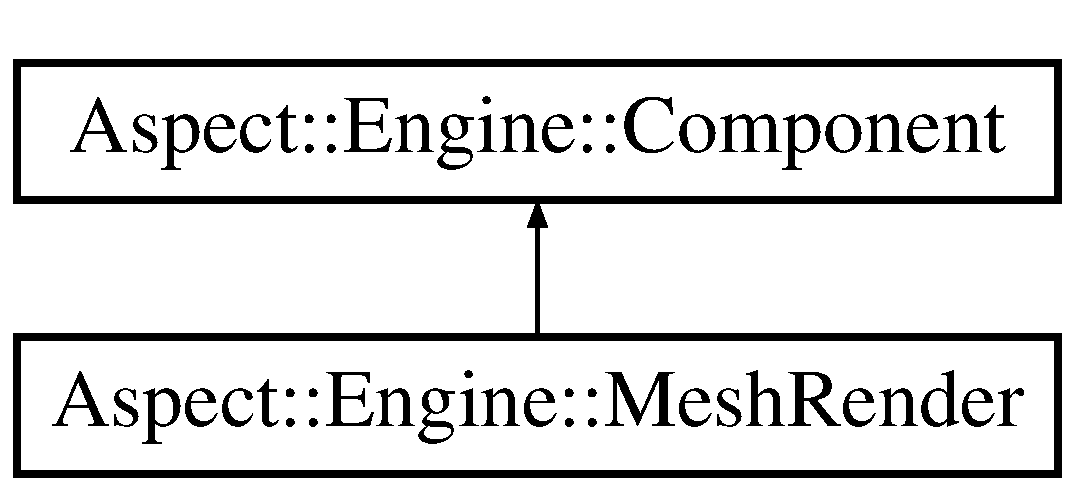
\includegraphics[height=1.230769cm]{class_aspect_1_1_engine_1_1_component}
\end{center}
\end{figure}
\subsection*{Public Member Functions}
\begin{DoxyCompactItemize}
\item 
virtual \mbox{\hyperlink{class_aspect_1_1_engine_1_1_component_a8ceb47c002468c4ad876b7220da579f8}{$\sim$\+Component}} ()
\item 
std\+::shared\+\_\+ptr$<$ \mbox{\hyperlink{class_aspect_1_1_engine_1_1_program}{Program}} $>$ \mbox{\hyperlink{class_aspect_1_1_engine_1_1_component_a96e352a6d49b6e108572c0c19088aa52}{get\+Program}} ()
\begin{DoxyCompactList}\small\item\em Class distructor. \end{DoxyCompactList}\item 
std\+::shared\+\_\+ptr$<$ \mbox{\hyperlink{class_aspect_1_1_engine_1_1_entity}{Entity}} $>$ \mbox{\hyperlink{class_aspect_1_1_engine_1_1_component_a1422571aabd1882f712e16ef4bf0cb77}{get\+Entity}} ()
\begin{DoxyCompactList}\small\item\em Creates a shared ptr function get\+Program. \end{DoxyCompactList}\item 
\mbox{\hyperlink{_s_d_l__opengles2__gl2ext_8h_ae5d8fa23ad07c48bb609509eae494c95}{void}} \mbox{\hyperlink{class_aspect_1_1_engine_1_1_component_accb4c932c2e93369ca168e1cd204ee31}{add\+Entity}} (std\+::weak\+\_\+ptr$<$ \mbox{\hyperlink{class_aspect_1_1_engine_1_1_entity}{Entity}} $>$ \+\_\+entity)
\begin{DoxyCompactList}\small\item\em Creates a shared ptr function to get\+Entiy. \end{DoxyCompactList}\end{DoxyCompactItemize}
\subsection*{Private Member Functions}
\begin{DoxyCompactItemize}
\item 
virtual \mbox{\hyperlink{_s_d_l__opengles2__gl2ext_8h_ae5d8fa23ad07c48bb609509eae494c95}{void}} \mbox{\hyperlink{class_aspect_1_1_engine_1_1_component_a3a1fbf76e3fd208be7ffe0ffa449dcf9}{on\+Init}} ()
\item 
virtual \mbox{\hyperlink{_s_d_l__opengles2__gl2ext_8h_ae5d8fa23ad07c48bb609509eae494c95}{void}} \mbox{\hyperlink{class_aspect_1_1_engine_1_1_component_a74ced87351b55406936e9d0009743557}{on\+Begin}} ()
\begin{DoxyCompactList}\small\item\em Initialise component function. \end{DoxyCompactList}\item 
virtual \mbox{\hyperlink{_s_d_l__opengles2__gl2ext_8h_ae5d8fa23ad07c48bb609509eae494c95}{void}} \mbox{\hyperlink{class_aspect_1_1_engine_1_1_component_a02de673a0591459bd0d39e3022c1d3fc}{on\+Count}} ()
\begin{DoxyCompactList}\small\item\em Begin function for components for entities. \end{DoxyCompactList}\item 
virtual \mbox{\hyperlink{_s_d_l__opengles2__gl2ext_8h_ae5d8fa23ad07c48bb609509eae494c95}{void}} \mbox{\hyperlink{class_aspect_1_1_engine_1_1_component_ac67307dba854cdc9535a0de75e5a3d09}{on\+Display}} ()
\begin{DoxyCompactList}\small\item\em On count same as update. \end{DoxyCompactList}\end{DoxyCompactItemize}
\subsection*{Private Attributes}
\begin{DoxyCompactItemize}
\item 
std\+::weak\+\_\+ptr$<$ \mbox{\hyperlink{class_aspect_1_1_engine_1_1_entity}{Entity}} $>$ \mbox{\hyperlink{class_aspect_1_1_engine_1_1_component_adc1d5c50c770bd9a173c0d63a61fe46c}{entity}}
\begin{DoxyCompactList}\small\item\em Creates the add entity function to add more entites to the program and entities list. \end{DoxyCompactList}\item 
bool \mbox{\hyperlink{class_aspect_1_1_engine_1_1_component_a648bedde21f792635f87889357fa2965}{m\+\_\+begin}}
\item 
\mbox{\hyperlink{group__core__types_ga7dcd2365c2e368e6af5b7adeb6a9c8df}{glm\+::mat4}} \mbox{\hyperlink{class_aspect_1_1_engine_1_1_component_a8307884a0e42764fd72af572e4ffdc7f}{view\+Matrix}}
\item 
float \mbox{\hyperlink{class_aspect_1_1_engine_1_1_component_ae5201488df91c23147632cc507b36c82}{camera\+AngleX}}
\item 
float \mbox{\hyperlink{class_aspect_1_1_engine_1_1_component_a9767131422976b1fb5b253c1ac114981}{camera\+AngleY}}
\end{DoxyCompactItemize}
\subsection*{Friends}
\begin{DoxyCompactItemize}
\item 
class \mbox{\hyperlink{class_aspect_1_1_engine_1_1_component_a614439ccac0344926adc4c0165d64060}{Entity}}
\end{DoxyCompactItemize}


\subsection{Detailed Description}
Initialise \mbox{\hyperlink{class_aspect_1_1_engine_1_1_program}{Program}} class rather than include. 

\mbox{\hyperlink{class_aspect_1_1_engine_1_1_component}{Component}} class 

\subsection{Constructor \& Destructor Documentation}
\mbox{\Hypertarget{class_aspect_1_1_engine_1_1_component_a8ceb47c002468c4ad876b7220da579f8}\label{class_aspect_1_1_engine_1_1_component_a8ceb47c002468c4ad876b7220da579f8}} 
\index{Aspect\+::\+Engine\+::\+Component@{Aspect\+::\+Engine\+::\+Component}!````~Component@{$\sim$\+Component}}
\index{````~Component@{$\sim$\+Component}!Aspect\+::\+Engine\+::\+Component@{Aspect\+::\+Engine\+::\+Component}}
\subsubsection{\texorpdfstring{$\sim$\+Component()}{~Component()}}
{\footnotesize\ttfamily Aspect\+::\+Engine\+::\+Component\+::$\sim$\+Component (\begin{DoxyParamCaption}{ }\end{DoxyParamCaption})\hspace{0.3cm}{\ttfamily [virtual]}}



\subsection{Member Function Documentation}
\mbox{\Hypertarget{class_aspect_1_1_engine_1_1_component_accb4c932c2e93369ca168e1cd204ee31}\label{class_aspect_1_1_engine_1_1_component_accb4c932c2e93369ca168e1cd204ee31}} 
\index{Aspect\+::\+Engine\+::\+Component@{Aspect\+::\+Engine\+::\+Component}!add\+Entity@{add\+Entity}}
\index{add\+Entity@{add\+Entity}!Aspect\+::\+Engine\+::\+Component@{Aspect\+::\+Engine\+::\+Component}}
\subsubsection{\texorpdfstring{add\+Entity()}{addEntity()}}
{\footnotesize\ttfamily \mbox{\hyperlink{_s_d_l__opengles2__gl2ext_8h_ae5d8fa23ad07c48bb609509eae494c95}{void}} Aspect\+::\+Engine\+::\+Component\+::add\+Entity (\begin{DoxyParamCaption}\item[{std\+::weak\+\_\+ptr$<$ \mbox{\hyperlink{class_aspect_1_1_engine_1_1_entity}{Entity}} $>$}]{\+\_\+entity }\end{DoxyParamCaption})}



Creates a shared ptr function to get\+Entiy. 

\mbox{\Hypertarget{class_aspect_1_1_engine_1_1_component_a1422571aabd1882f712e16ef4bf0cb77}\label{class_aspect_1_1_engine_1_1_component_a1422571aabd1882f712e16ef4bf0cb77}} 
\index{Aspect\+::\+Engine\+::\+Component@{Aspect\+::\+Engine\+::\+Component}!get\+Entity@{get\+Entity}}
\index{get\+Entity@{get\+Entity}!Aspect\+::\+Engine\+::\+Component@{Aspect\+::\+Engine\+::\+Component}}
\subsubsection{\texorpdfstring{get\+Entity()}{getEntity()}}
{\footnotesize\ttfamily std\+::shared\+\_\+ptr$<$ \mbox{\hyperlink{class_aspect_1_1_engine_1_1_entity}{Entity}} $>$ Aspect\+::\+Engine\+::\+Component\+::get\+Entity (\begin{DoxyParamCaption}{ }\end{DoxyParamCaption})}



Creates a shared ptr function get\+Program. 

\mbox{\Hypertarget{class_aspect_1_1_engine_1_1_component_a96e352a6d49b6e108572c0c19088aa52}\label{class_aspect_1_1_engine_1_1_component_a96e352a6d49b6e108572c0c19088aa52}} 
\index{Aspect\+::\+Engine\+::\+Component@{Aspect\+::\+Engine\+::\+Component}!get\+Program@{get\+Program}}
\index{get\+Program@{get\+Program}!Aspect\+::\+Engine\+::\+Component@{Aspect\+::\+Engine\+::\+Component}}
\subsubsection{\texorpdfstring{get\+Program()}{getProgram()}}
{\footnotesize\ttfamily std\+::shared\+\_\+ptr$<$ \mbox{\hyperlink{class_aspect_1_1_engine_1_1_program}{Program}} $>$ Aspect\+::\+Engine\+::\+Component\+::get\+Program (\begin{DoxyParamCaption}{ }\end{DoxyParamCaption})}



Class distructor. 

\mbox{\Hypertarget{class_aspect_1_1_engine_1_1_component_a74ced87351b55406936e9d0009743557}\label{class_aspect_1_1_engine_1_1_component_a74ced87351b55406936e9d0009743557}} 
\index{Aspect\+::\+Engine\+::\+Component@{Aspect\+::\+Engine\+::\+Component}!on\+Begin@{on\+Begin}}
\index{on\+Begin@{on\+Begin}!Aspect\+::\+Engine\+::\+Component@{Aspect\+::\+Engine\+::\+Component}}
\subsubsection{\texorpdfstring{on\+Begin()}{onBegin()}}
{\footnotesize\ttfamily \mbox{\hyperlink{_s_d_l__opengles2__gl2ext_8h_ae5d8fa23ad07c48bb609509eae494c95}{void}} Aspect\+::\+Engine\+::\+Component\+::on\+Begin (\begin{DoxyParamCaption}{ }\end{DoxyParamCaption})\hspace{0.3cm}{\ttfamily [private]}, {\ttfamily [virtual]}}



Initialise component function. 

\mbox{\Hypertarget{class_aspect_1_1_engine_1_1_component_a02de673a0591459bd0d39e3022c1d3fc}\label{class_aspect_1_1_engine_1_1_component_a02de673a0591459bd0d39e3022c1d3fc}} 
\index{Aspect\+::\+Engine\+::\+Component@{Aspect\+::\+Engine\+::\+Component}!on\+Count@{on\+Count}}
\index{on\+Count@{on\+Count}!Aspect\+::\+Engine\+::\+Component@{Aspect\+::\+Engine\+::\+Component}}
\subsubsection{\texorpdfstring{on\+Count()}{onCount()}}
{\footnotesize\ttfamily \mbox{\hyperlink{_s_d_l__opengles2__gl2ext_8h_ae5d8fa23ad07c48bb609509eae494c95}{void}} Aspect\+::\+Engine\+::\+Component\+::on\+Count (\begin{DoxyParamCaption}{ }\end{DoxyParamCaption})\hspace{0.3cm}{\ttfamily [private]}, {\ttfamily [virtual]}}



Begin function for components for entities. 



Reimplemented in \mbox{\hyperlink{class_aspect_1_1_engine_1_1_mesh_render_aebaa5a60d373d3363a13336cfbaa4141}{Aspect\+::\+Engine\+::\+Mesh\+Render}}, \mbox{\hyperlink{class_aspect_1_1_engine_1_1_transform_acb53a815498eea17774cc42cfa6c03bd}{Aspect\+::\+Engine\+::\+Transform}}, and \mbox{\hyperlink{class_aspect_1_1_engine_1_1_movement_a4dc9ec0157d8d24dafeb69c3c3f60e23}{Aspect\+::\+Engine\+::\+Movement}}.

\mbox{\Hypertarget{class_aspect_1_1_engine_1_1_component_ac67307dba854cdc9535a0de75e5a3d09}\label{class_aspect_1_1_engine_1_1_component_ac67307dba854cdc9535a0de75e5a3d09}} 
\index{Aspect\+::\+Engine\+::\+Component@{Aspect\+::\+Engine\+::\+Component}!on\+Display@{on\+Display}}
\index{on\+Display@{on\+Display}!Aspect\+::\+Engine\+::\+Component@{Aspect\+::\+Engine\+::\+Component}}
\subsubsection{\texorpdfstring{on\+Display()}{onDisplay()}}
{\footnotesize\ttfamily \mbox{\hyperlink{_s_d_l__opengles2__gl2ext_8h_ae5d8fa23ad07c48bb609509eae494c95}{void}} Aspect\+::\+Engine\+::\+Component\+::on\+Display (\begin{DoxyParamCaption}{ }\end{DoxyParamCaption})\hspace{0.3cm}{\ttfamily [private]}, {\ttfamily [virtual]}}



On count same as update. 



Reimplemented in \mbox{\hyperlink{class_aspect_1_1_engine_1_1_mesh_render_aed81ecbd6bf1d63acb06171f729e4927}{Aspect\+::\+Engine\+::\+Mesh\+Render}}.

\mbox{\Hypertarget{class_aspect_1_1_engine_1_1_component_a3a1fbf76e3fd208be7ffe0ffa449dcf9}\label{class_aspect_1_1_engine_1_1_component_a3a1fbf76e3fd208be7ffe0ffa449dcf9}} 
\index{Aspect\+::\+Engine\+::\+Component@{Aspect\+::\+Engine\+::\+Component}!on\+Init@{on\+Init}}
\index{on\+Init@{on\+Init}!Aspect\+::\+Engine\+::\+Component@{Aspect\+::\+Engine\+::\+Component}}
\subsubsection{\texorpdfstring{on\+Init()}{onInit()}}
{\footnotesize\ttfamily \mbox{\hyperlink{_s_d_l__opengles2__gl2ext_8h_ae5d8fa23ad07c48bb609509eae494c95}{void}} Aspect\+::\+Engine\+::\+Component\+::on\+Init (\begin{DoxyParamCaption}{ }\end{DoxyParamCaption})\hspace{0.3cm}{\ttfamily [private]}, {\ttfamily [virtual]}}



Reimplemented in \mbox{\hyperlink{class_aspect_1_1_engine_1_1_mesh_render_a54bb4394dafdc30e919a0ba5d9854871}{Aspect\+::\+Engine\+::\+Mesh\+Render}}, and \mbox{\hyperlink{class_aspect_1_1_engine_1_1_camera_a30e0d0ecb4c5c9fd43cfe8323e600d17}{Aspect\+::\+Engine\+::\+Camera}}.



\subsection{Friends And Related Function Documentation}
\mbox{\Hypertarget{class_aspect_1_1_engine_1_1_component_a614439ccac0344926adc4c0165d64060}\label{class_aspect_1_1_engine_1_1_component_a614439ccac0344926adc4c0165d64060}} 
\index{Aspect\+::\+Engine\+::\+Component@{Aspect\+::\+Engine\+::\+Component}!Entity@{Entity}}
\index{Entity@{Entity}!Aspect\+::\+Engine\+::\+Component@{Aspect\+::\+Engine\+::\+Component}}
\subsubsection{\texorpdfstring{Entity}{Entity}}
{\footnotesize\ttfamily friend class \mbox{\hyperlink{class_aspect_1_1_engine_1_1_entity}{Entity}}\hspace{0.3cm}{\ttfamily [friend]}}



\subsection{Member Data Documentation}
\mbox{\Hypertarget{class_aspect_1_1_engine_1_1_component_ae5201488df91c23147632cc507b36c82}\label{class_aspect_1_1_engine_1_1_component_ae5201488df91c23147632cc507b36c82}} 
\index{Aspect\+::\+Engine\+::\+Component@{Aspect\+::\+Engine\+::\+Component}!camera\+AngleX@{camera\+AngleX}}
\index{camera\+AngleX@{camera\+AngleX}!Aspect\+::\+Engine\+::\+Component@{Aspect\+::\+Engine\+::\+Component}}
\subsubsection{\texorpdfstring{camera\+AngleX}{cameraAngleX}}
{\footnotesize\ttfamily float Aspect\+::\+Engine\+::\+Component\+::camera\+AngleX\hspace{0.3cm}{\ttfamily [private]}}

\mbox{\Hypertarget{class_aspect_1_1_engine_1_1_component_a9767131422976b1fb5b253c1ac114981}\label{class_aspect_1_1_engine_1_1_component_a9767131422976b1fb5b253c1ac114981}} 
\index{Aspect\+::\+Engine\+::\+Component@{Aspect\+::\+Engine\+::\+Component}!camera\+AngleY@{camera\+AngleY}}
\index{camera\+AngleY@{camera\+AngleY}!Aspect\+::\+Engine\+::\+Component@{Aspect\+::\+Engine\+::\+Component}}
\subsubsection{\texorpdfstring{camera\+AngleY}{cameraAngleY}}
{\footnotesize\ttfamily float Aspect\+::\+Engine\+::\+Component\+::camera\+AngleY\hspace{0.3cm}{\ttfamily [private]}}

\mbox{\Hypertarget{class_aspect_1_1_engine_1_1_component_adc1d5c50c770bd9a173c0d63a61fe46c}\label{class_aspect_1_1_engine_1_1_component_adc1d5c50c770bd9a173c0d63a61fe46c}} 
\index{Aspect\+::\+Engine\+::\+Component@{Aspect\+::\+Engine\+::\+Component}!entity@{entity}}
\index{entity@{entity}!Aspect\+::\+Engine\+::\+Component@{Aspect\+::\+Engine\+::\+Component}}
\subsubsection{\texorpdfstring{entity}{entity}}
{\footnotesize\ttfamily std\+::weak\+\_\+ptr$<$\mbox{\hyperlink{class_aspect_1_1_engine_1_1_entity}{Entity}}$>$ Aspect\+::\+Engine\+::\+Component\+::entity\hspace{0.3cm}{\ttfamily [private]}}



Creates the add entity function to add more entites to the program and entities list. 

\mbox{\Hypertarget{class_aspect_1_1_engine_1_1_component_a648bedde21f792635f87889357fa2965}\label{class_aspect_1_1_engine_1_1_component_a648bedde21f792635f87889357fa2965}} 
\index{Aspect\+::\+Engine\+::\+Component@{Aspect\+::\+Engine\+::\+Component}!m\+\_\+begin@{m\+\_\+begin}}
\index{m\+\_\+begin@{m\+\_\+begin}!Aspect\+::\+Engine\+::\+Component@{Aspect\+::\+Engine\+::\+Component}}
\subsubsection{\texorpdfstring{m\+\_\+begin}{m\_begin}}
{\footnotesize\ttfamily bool Aspect\+::\+Engine\+::\+Component\+::m\+\_\+begin\hspace{0.3cm}{\ttfamily [private]}}

\mbox{\Hypertarget{class_aspect_1_1_engine_1_1_component_a8307884a0e42764fd72af572e4ffdc7f}\label{class_aspect_1_1_engine_1_1_component_a8307884a0e42764fd72af572e4ffdc7f}} 
\index{Aspect\+::\+Engine\+::\+Component@{Aspect\+::\+Engine\+::\+Component}!view\+Matrix@{view\+Matrix}}
\index{view\+Matrix@{view\+Matrix}!Aspect\+::\+Engine\+::\+Component@{Aspect\+::\+Engine\+::\+Component}}
\subsubsection{\texorpdfstring{view\+Matrix}{viewMatrix}}
{\footnotesize\ttfamily \mbox{\hyperlink{group__core__types_ga7dcd2365c2e368e6af5b7adeb6a9c8df}{glm\+::mat4}} Aspect\+::\+Engine\+::\+Component\+::view\+Matrix\hspace{0.3cm}{\ttfamily [private]}}



The documentation for this class was generated from the following files\+:\begin{DoxyCompactItemize}
\item 
src/\+Aspect/\mbox{\hyperlink{_component_8h}{Component.\+h}}\item 
src/\+Aspect/\mbox{\hyperlink{_component_8cpp}{Component.\+cpp}}\end{DoxyCompactItemize}

\hypertarget{class_aspect_1_1_engine_1_1_entity}{}\section{Aspect\+:\+:Engine\+:\+:Entity Class Reference}
\label{class_aspect_1_1_engine_1_1_entity}\index{Aspect\+::\+Engine\+::\+Entity@{Aspect\+::\+Engine\+::\+Entity}}


Initialise the component class.  




{\ttfamily \#include $<$Entity.\+h$>$}

\subsection*{Public Member Functions}
\begin{DoxyCompactItemize}
\item 
{\footnotesize template$<$typename T $>$ }\\std\+::shared\+\_\+ptr$<$ T $>$ \mbox{\hyperlink{class_aspect_1_1_engine_1_1_entity_a5fdedcbe74684afa991dc83b6c7b96a1}{get\+Component}} ()
\begin{DoxyCompactList}\small\item\em Type T Template class to get a single component. \end{DoxyCompactList}\item 
{\footnotesize template$<$typename T $>$ }\\bool \mbox{\hyperlink{class_aspect_1_1_engine_1_1_entity_accfb5d56f8f88f9007504e580120a777}{has\+Component}} ()
\begin{DoxyCompactList}\small\item\em Type T Template class to get a single component. \end{DoxyCompactList}\item 
{\footnotesize template$<$typename T $>$ }\\std\+::shared\+\_\+ptr$<$ T $>$ \mbox{\hyperlink{class_aspect_1_1_engine_1_1_entity_ae7a087ed64f4fec3b61ff2cba098d19a}{add\+Component}} ()
\begin{DoxyCompactList}\small\item\em Type t template class to add a single component. \end{DoxyCompactList}\item 
{\footnotesize template$<$typename T , typename A $>$ }\\std\+::shared\+\_\+ptr$<$ T $>$ \mbox{\hyperlink{class_aspect_1_1_engine_1_1_entity_aac44f29e1ad32261d7853e59a7562671}{add\+Component}} (A \mbox{\hyperlink{_s_d_l__opengl__glext_8h_a3309789fc188587d666cda5ece79cf82}{a}})
\begin{DoxyCompactList}\small\item\em Type t template class to add 2 components. \end{DoxyCompactList}\item 
{\footnotesize template$<$typename T , typename A , typename B $>$ }\\std\+::shared\+\_\+ptr$<$ T $>$ \mbox{\hyperlink{class_aspect_1_1_engine_1_1_entity_a73a023e500fddd340cf843e6e11796dd}{add\+Component}} (A \mbox{\hyperlink{_s_d_l__opengl__glext_8h_a3309789fc188587d666cda5ece79cf82}{a}}, B \mbox{\hyperlink{_s_d_l__opengl__glext_8h_a0f71581a41fd2264c8944126dabbd010}{b}})
\begin{DoxyCompactList}\small\item\em Type t template class to add 3 components. \end{DoxyCompactList}\item 
\mbox{\hyperlink{_s_d_l__opengles2__gl2ext_8h_ae5d8fa23ad07c48bb609509eae494c95}{void}} \mbox{\hyperlink{class_aspect_1_1_engine_1_1_entity_ad3a033d6bbe1dfa9011e4f2d5ce8c928}{count}} ()
\item 
\mbox{\hyperlink{_s_d_l__opengles2__gl2ext_8h_ae5d8fa23ad07c48bb609509eae494c95}{void}} \mbox{\hyperlink{class_aspect_1_1_engine_1_1_entity_ac889f58ccf361ce3ec1126f9df141679}{display}} ()
\begin{DoxyCompactList}\small\item\em Update function. \end{DoxyCompactList}\item 
\mbox{\hyperlink{_s_d_l__opengles2__gl2ext_8h_ae5d8fa23ad07c48bb609509eae494c95}{void}} \mbox{\hyperlink{class_aspect_1_1_engine_1_1_entity_a9e6f9d5884b67082bcafc76b6cfacd79}{set\+Destroy}} (bool \mbox{\hyperlink{class_aspect_1_1_engine_1_1_entity_a425294ababc4132392204443f47cb36a}{destroy}})
\begin{DoxyCompactList}\small\item\em Draw function. \end{DoxyCompactList}\item 
bool \mbox{\hyperlink{class_aspect_1_1_engine_1_1_entity_a62a6db91aaf6b188d57edeb2bfa24767}{is\+Destroyed}} ()
\begin{DoxyCompactList}\small\item\em Destory game objects. \end{DoxyCompactList}\item 
std\+::shared\+\_\+ptr$<$ \mbox{\hyperlink{class_aspect_1_1_engine_1_1_program}{Program}} $>$ \mbox{\hyperlink{class_aspect_1_1_engine_1_1_entity_a39566f856dd82efb948383c3037290a0}{get\+Program}} ()
\end{DoxyCompactItemize}
\subsection*{Public Attributes}
\begin{DoxyCompactItemize}
\item 
bool \mbox{\hyperlink{class_aspect_1_1_engine_1_1_entity_a425294ababc4132392204443f47cb36a}{destroy}}
\item 
std\+::vector$<$ std\+::shared\+\_\+ptr$<$ \mbox{\hyperlink{class_aspect_1_1_engine_1_1_component}{Component}} $>$ $>$ \mbox{\hyperlink{class_aspect_1_1_engine_1_1_entity_ae7380f6b33ebbb9d4859a9de11549769}{components}}
\item 
std\+::weak\+\_\+ptr$<$ \mbox{\hyperlink{class_aspect_1_1_engine_1_1_program}{Program}} $>$ \mbox{\hyperlink{class_aspect_1_1_engine_1_1_entity_a39a0c787c384f192878e9c16f566b892}{program}}
\begin{DoxyCompactList}\small\item\em Get program function. \end{DoxyCompactList}\item 
std\+::weak\+\_\+ptr$<$ \mbox{\hyperlink{class_aspect_1_1_engine_1_1_entity}{Entity}} $>$ \mbox{\hyperlink{class_aspect_1_1_engine_1_1_entity_a23ba239d52c76b8c7f86a4ebdd189d26}{self}}
\end{DoxyCompactItemize}


\subsection{Detailed Description}
Initialise the component class. 

Initialise the entity class 

\subsection{Member Function Documentation}
\mbox{\Hypertarget{class_aspect_1_1_engine_1_1_entity_ae7a087ed64f4fec3b61ff2cba098d19a}\label{class_aspect_1_1_engine_1_1_entity_ae7a087ed64f4fec3b61ff2cba098d19a}} 
\index{Aspect\+::\+Engine\+::\+Entity@{Aspect\+::\+Engine\+::\+Entity}!add\+Component@{add\+Component}}
\index{add\+Component@{add\+Component}!Aspect\+::\+Engine\+::\+Entity@{Aspect\+::\+Engine\+::\+Entity}}
\subsubsection{\texorpdfstring{add\+Component()}{addComponent()}\hspace{0.1cm}{\footnotesize\ttfamily [1/3]}}
{\footnotesize\ttfamily template$<$typename T $>$ \\
std\+::shared\+\_\+ptr$<$T$>$ Aspect\+::\+Engine\+::\+Entity\+::add\+Component (\begin{DoxyParamCaption}{ }\end{DoxyParamCaption})\hspace{0.3cm}{\ttfamily [inline]}}



Type t template class to add a single component. 

\mbox{\Hypertarget{class_aspect_1_1_engine_1_1_entity_aac44f29e1ad32261d7853e59a7562671}\label{class_aspect_1_1_engine_1_1_entity_aac44f29e1ad32261d7853e59a7562671}} 
\index{Aspect\+::\+Engine\+::\+Entity@{Aspect\+::\+Engine\+::\+Entity}!add\+Component@{add\+Component}}
\index{add\+Component@{add\+Component}!Aspect\+::\+Engine\+::\+Entity@{Aspect\+::\+Engine\+::\+Entity}}
\subsubsection{\texorpdfstring{add\+Component()}{addComponent()}\hspace{0.1cm}{\footnotesize\ttfamily [2/3]}}
{\footnotesize\ttfamily template$<$typename T , typename A $>$ \\
std\+::shared\+\_\+ptr$<$T$>$ Aspect\+::\+Engine\+::\+Entity\+::add\+Component (\begin{DoxyParamCaption}\item[{A}]{a }\end{DoxyParamCaption})\hspace{0.3cm}{\ttfamily [inline]}}



Type t template class to add 2 components. 

\mbox{\Hypertarget{class_aspect_1_1_engine_1_1_entity_a73a023e500fddd340cf843e6e11796dd}\label{class_aspect_1_1_engine_1_1_entity_a73a023e500fddd340cf843e6e11796dd}} 
\index{Aspect\+::\+Engine\+::\+Entity@{Aspect\+::\+Engine\+::\+Entity}!add\+Component@{add\+Component}}
\index{add\+Component@{add\+Component}!Aspect\+::\+Engine\+::\+Entity@{Aspect\+::\+Engine\+::\+Entity}}
\subsubsection{\texorpdfstring{add\+Component()}{addComponent()}\hspace{0.1cm}{\footnotesize\ttfamily [3/3]}}
{\footnotesize\ttfamily template$<$typename T , typename A , typename B $>$ \\
std\+::shared\+\_\+ptr$<$T$>$ Aspect\+::\+Engine\+::\+Entity\+::add\+Component (\begin{DoxyParamCaption}\item[{A}]{a,  }\item[{B}]{b }\end{DoxyParamCaption})\hspace{0.3cm}{\ttfamily [inline]}}



Type t template class to add 3 components. 

\mbox{\Hypertarget{class_aspect_1_1_engine_1_1_entity_ad3a033d6bbe1dfa9011e4f2d5ce8c928}\label{class_aspect_1_1_engine_1_1_entity_ad3a033d6bbe1dfa9011e4f2d5ce8c928}} 
\index{Aspect\+::\+Engine\+::\+Entity@{Aspect\+::\+Engine\+::\+Entity}!count@{count}}
\index{count@{count}!Aspect\+::\+Engine\+::\+Entity@{Aspect\+::\+Engine\+::\+Entity}}
\subsubsection{\texorpdfstring{count()}{count()}}
{\footnotesize\ttfamily \mbox{\hyperlink{_s_d_l__opengles2__gl2ext_8h_ae5d8fa23ad07c48bb609509eae494c95}{void}} Aspect\+::\+Engine\+::\+Entity\+::count (\begin{DoxyParamCaption}{ }\end{DoxyParamCaption})}

\mbox{\Hypertarget{class_aspect_1_1_engine_1_1_entity_ac889f58ccf361ce3ec1126f9df141679}\label{class_aspect_1_1_engine_1_1_entity_ac889f58ccf361ce3ec1126f9df141679}} 
\index{Aspect\+::\+Engine\+::\+Entity@{Aspect\+::\+Engine\+::\+Entity}!display@{display}}
\index{display@{display}!Aspect\+::\+Engine\+::\+Entity@{Aspect\+::\+Engine\+::\+Entity}}
\subsubsection{\texorpdfstring{display()}{display()}}
{\footnotesize\ttfamily \mbox{\hyperlink{_s_d_l__opengles2__gl2ext_8h_ae5d8fa23ad07c48bb609509eae494c95}{void}} Aspect\+::\+Engine\+::\+Entity\+::display (\begin{DoxyParamCaption}{ }\end{DoxyParamCaption})}



Update function. 

\mbox{\Hypertarget{class_aspect_1_1_engine_1_1_entity_a5fdedcbe74684afa991dc83b6c7b96a1}\label{class_aspect_1_1_engine_1_1_entity_a5fdedcbe74684afa991dc83b6c7b96a1}} 
\index{Aspect\+::\+Engine\+::\+Entity@{Aspect\+::\+Engine\+::\+Entity}!get\+Component@{get\+Component}}
\index{get\+Component@{get\+Component}!Aspect\+::\+Engine\+::\+Entity@{Aspect\+::\+Engine\+::\+Entity}}
\subsubsection{\texorpdfstring{get\+Component()}{getComponent()}}
{\footnotesize\ttfamily template$<$typename T $>$ \\
std\+::shared\+\_\+ptr$<$T$>$ Aspect\+::\+Engine\+::\+Entity\+::get\+Component (\begin{DoxyParamCaption}{ }\end{DoxyParamCaption})\hspace{0.3cm}{\ttfamily [inline]}}



Type T Template class to get a single component. 

\mbox{\Hypertarget{class_aspect_1_1_engine_1_1_entity_a39566f856dd82efb948383c3037290a0}\label{class_aspect_1_1_engine_1_1_entity_a39566f856dd82efb948383c3037290a0}} 
\index{Aspect\+::\+Engine\+::\+Entity@{Aspect\+::\+Engine\+::\+Entity}!get\+Program@{get\+Program}}
\index{get\+Program@{get\+Program}!Aspect\+::\+Engine\+::\+Entity@{Aspect\+::\+Engine\+::\+Entity}}
\subsubsection{\texorpdfstring{get\+Program()}{getProgram()}}
{\footnotesize\ttfamily std\+::shared\+\_\+ptr$<$ \mbox{\hyperlink{class_aspect_1_1_engine_1_1_program}{Program}} $>$ Aspect\+::\+Engine\+::\+Entity\+::get\+Program (\begin{DoxyParamCaption}{ }\end{DoxyParamCaption})}

\mbox{\Hypertarget{class_aspect_1_1_engine_1_1_entity_accfb5d56f8f88f9007504e580120a777}\label{class_aspect_1_1_engine_1_1_entity_accfb5d56f8f88f9007504e580120a777}} 
\index{Aspect\+::\+Engine\+::\+Entity@{Aspect\+::\+Engine\+::\+Entity}!has\+Component@{has\+Component}}
\index{has\+Component@{has\+Component}!Aspect\+::\+Engine\+::\+Entity@{Aspect\+::\+Engine\+::\+Entity}}
\subsubsection{\texorpdfstring{has\+Component()}{hasComponent()}}
{\footnotesize\ttfamily template$<$typename T $>$ \\
bool Aspect\+::\+Engine\+::\+Entity\+::has\+Component (\begin{DoxyParamCaption}{ }\end{DoxyParamCaption})\hspace{0.3cm}{\ttfamily [inline]}}



Type T Template class to get a single component. 

\mbox{\Hypertarget{class_aspect_1_1_engine_1_1_entity_a62a6db91aaf6b188d57edeb2bfa24767}\label{class_aspect_1_1_engine_1_1_entity_a62a6db91aaf6b188d57edeb2bfa24767}} 
\index{Aspect\+::\+Engine\+::\+Entity@{Aspect\+::\+Engine\+::\+Entity}!is\+Destroyed@{is\+Destroyed}}
\index{is\+Destroyed@{is\+Destroyed}!Aspect\+::\+Engine\+::\+Entity@{Aspect\+::\+Engine\+::\+Entity}}
\subsubsection{\texorpdfstring{is\+Destroyed()}{isDestroyed()}}
{\footnotesize\ttfamily bool Aspect\+::\+Engine\+::\+Entity\+::is\+Destroyed (\begin{DoxyParamCaption}{ }\end{DoxyParamCaption})\hspace{0.3cm}{\ttfamily [inline]}}



Destory game objects. 

\mbox{\Hypertarget{class_aspect_1_1_engine_1_1_entity_a9e6f9d5884b67082bcafc76b6cfacd79}\label{class_aspect_1_1_engine_1_1_entity_a9e6f9d5884b67082bcafc76b6cfacd79}} 
\index{Aspect\+::\+Engine\+::\+Entity@{Aspect\+::\+Engine\+::\+Entity}!set\+Destroy@{set\+Destroy}}
\index{set\+Destroy@{set\+Destroy}!Aspect\+::\+Engine\+::\+Entity@{Aspect\+::\+Engine\+::\+Entity}}
\subsubsection{\texorpdfstring{set\+Destroy()}{setDestroy()}}
{\footnotesize\ttfamily \mbox{\hyperlink{_s_d_l__opengles2__gl2ext_8h_ae5d8fa23ad07c48bb609509eae494c95}{void}} Aspect\+::\+Engine\+::\+Entity\+::set\+Destroy (\begin{DoxyParamCaption}\item[{bool}]{destroy }\end{DoxyParamCaption})\hspace{0.3cm}{\ttfamily [inline]}}



Draw function. 



\subsection{Member Data Documentation}
\mbox{\Hypertarget{class_aspect_1_1_engine_1_1_entity_ae7380f6b33ebbb9d4859a9de11549769}\label{class_aspect_1_1_engine_1_1_entity_ae7380f6b33ebbb9d4859a9de11549769}} 
\index{Aspect\+::\+Engine\+::\+Entity@{Aspect\+::\+Engine\+::\+Entity}!components@{components}}
\index{components@{components}!Aspect\+::\+Engine\+::\+Entity@{Aspect\+::\+Engine\+::\+Entity}}
\subsubsection{\texorpdfstring{components}{components}}
{\footnotesize\ttfamily std\+::vector$<$std\+::shared\+\_\+ptr$<$\mbox{\hyperlink{class_aspect_1_1_engine_1_1_component}{Component}}$>$ $>$ Aspect\+::\+Engine\+::\+Entity\+::components}

\mbox{\Hypertarget{class_aspect_1_1_engine_1_1_entity_a425294ababc4132392204443f47cb36a}\label{class_aspect_1_1_engine_1_1_entity_a425294ababc4132392204443f47cb36a}} 
\index{Aspect\+::\+Engine\+::\+Entity@{Aspect\+::\+Engine\+::\+Entity}!destroy@{destroy}}
\index{destroy@{destroy}!Aspect\+::\+Engine\+::\+Entity@{Aspect\+::\+Engine\+::\+Entity}}
\subsubsection{\texorpdfstring{destroy}{destroy}}
{\footnotesize\ttfamily bool Aspect\+::\+Engine\+::\+Entity\+::destroy}

\mbox{\Hypertarget{class_aspect_1_1_engine_1_1_entity_a39a0c787c384f192878e9c16f566b892}\label{class_aspect_1_1_engine_1_1_entity_a39a0c787c384f192878e9c16f566b892}} 
\index{Aspect\+::\+Engine\+::\+Entity@{Aspect\+::\+Engine\+::\+Entity}!program@{program}}
\index{program@{program}!Aspect\+::\+Engine\+::\+Entity@{Aspect\+::\+Engine\+::\+Entity}}
\subsubsection{\texorpdfstring{program}{program}}
{\footnotesize\ttfamily std\+::weak\+\_\+ptr$<$\mbox{\hyperlink{class_aspect_1_1_engine_1_1_program}{Program}}$>$ Aspect\+::\+Engine\+::\+Entity\+::program}



Get program function. 

\mbox{\Hypertarget{class_aspect_1_1_engine_1_1_entity_a23ba239d52c76b8c7f86a4ebdd189d26}\label{class_aspect_1_1_engine_1_1_entity_a23ba239d52c76b8c7f86a4ebdd189d26}} 
\index{Aspect\+::\+Engine\+::\+Entity@{Aspect\+::\+Engine\+::\+Entity}!self@{self}}
\index{self@{self}!Aspect\+::\+Engine\+::\+Entity@{Aspect\+::\+Engine\+::\+Entity}}
\subsubsection{\texorpdfstring{self}{self}}
{\footnotesize\ttfamily std\+::weak\+\_\+ptr$<$\mbox{\hyperlink{class_aspect_1_1_engine_1_1_entity}{Entity}}$>$ Aspect\+::\+Engine\+::\+Entity\+::self}



The documentation for this class was generated from the following files\+:\begin{DoxyCompactItemize}
\item 
src/\+Aspect/\mbox{\hyperlink{_entity_8h}{Entity.\+h}}\item 
src/\+Aspect/\mbox{\hyperlink{_entity_8cpp}{Entity.\+cpp}}\end{DoxyCompactItemize}

\hypertarget{class_aspect_1_1_engine_1_1_material}{}\section{Aspect\+:\+:Engine\+:\+:Material Class Reference}
\label{class_aspect_1_1_engine_1_1_material}\index{Aspect\+::\+Engine\+::\+Material@{Aspect\+::\+Engine\+::\+Material}}


{\ttfamily \#include $<$Material.\+h$>$}

\subsection*{Public Member Functions}
\begin{DoxyCompactItemize}
\item 
\mbox{\hyperlink{class_aspect_1_1_engine_1_1_material_a2c9f3f523dc327399c24b4222d4a978c}{Material}} (std\+::string path)
\item 
glm\+::vec2 \mbox{\hyperlink{class_aspect_1_1_engine_1_1_material_a8779008ace71c3d1ee2cd551373933be}{get\+Size}} ()
\item 
G\+Luint \mbox{\hyperlink{class_aspect_1_1_engine_1_1_material_ac4177400efde4d6ced260e707b3e5ad0}{get\+Id}} ()
\end{DoxyCompactItemize}
\subsection*{Public Attributes}
\begin{DoxyCompactItemize}
\item 
int \mbox{\hyperlink{class_aspect_1_1_engine_1_1_material_a2c52f153e9878530ae68627c9a1f16be}{w}}
\item 
int \mbox{\hyperlink{class_aspect_1_1_engine_1_1_material_a495fcbe4e64c1814971cd9d815dd0e16}{h}}
\item 
int \mbox{\hyperlink{class_aspect_1_1_engine_1_1_material_ae0b4f29080da1fdfb87763c8b72f3110}{channels}}
\end{DoxyCompactItemize}


\subsection{Constructor \& Destructor Documentation}
\mbox{\Hypertarget{class_aspect_1_1_engine_1_1_material_a2c9f3f523dc327399c24b4222d4a978c}\label{class_aspect_1_1_engine_1_1_material_a2c9f3f523dc327399c24b4222d4a978c}} 
\index{Aspect\+::\+Engine\+::\+Material@{Aspect\+::\+Engine\+::\+Material}!Material@{Material}}
\index{Material@{Material}!Aspect\+::\+Engine\+::\+Material@{Aspect\+::\+Engine\+::\+Material}}
\subsubsection{\texorpdfstring{Material()}{Material()}}
{\footnotesize\ttfamily Aspect\+::\+Engine\+::\+Material\+::\+Material (\begin{DoxyParamCaption}\item[{std\+::string}]{path }\end{DoxyParamCaption})}



\subsection{Member Function Documentation}
\mbox{\Hypertarget{class_aspect_1_1_engine_1_1_material_ac4177400efde4d6ced260e707b3e5ad0}\label{class_aspect_1_1_engine_1_1_material_ac4177400efde4d6ced260e707b3e5ad0}} 
\index{Aspect\+::\+Engine\+::\+Material@{Aspect\+::\+Engine\+::\+Material}!get\+Id@{get\+Id}}
\index{get\+Id@{get\+Id}!Aspect\+::\+Engine\+::\+Material@{Aspect\+::\+Engine\+::\+Material}}
\subsubsection{\texorpdfstring{get\+Id()}{getId()}}
{\footnotesize\ttfamily G\+Luint Aspect\+::\+Engine\+::\+Material\+::get\+Id (\begin{DoxyParamCaption}{ }\end{DoxyParamCaption})}

\mbox{\Hypertarget{class_aspect_1_1_engine_1_1_material_a8779008ace71c3d1ee2cd551373933be}\label{class_aspect_1_1_engine_1_1_material_a8779008ace71c3d1ee2cd551373933be}} 
\index{Aspect\+::\+Engine\+::\+Material@{Aspect\+::\+Engine\+::\+Material}!get\+Size@{get\+Size}}
\index{get\+Size@{get\+Size}!Aspect\+::\+Engine\+::\+Material@{Aspect\+::\+Engine\+::\+Material}}
\subsubsection{\texorpdfstring{get\+Size()}{getSize()}}
{\footnotesize\ttfamily glm\+::vec2 Aspect\+::\+Engine\+::\+Material\+::get\+Size (\begin{DoxyParamCaption}{ }\end{DoxyParamCaption})}



\subsection{Member Data Documentation}
\mbox{\Hypertarget{class_aspect_1_1_engine_1_1_material_ae0b4f29080da1fdfb87763c8b72f3110}\label{class_aspect_1_1_engine_1_1_material_ae0b4f29080da1fdfb87763c8b72f3110}} 
\index{Aspect\+::\+Engine\+::\+Material@{Aspect\+::\+Engine\+::\+Material}!channels@{channels}}
\index{channels@{channels}!Aspect\+::\+Engine\+::\+Material@{Aspect\+::\+Engine\+::\+Material}}
\subsubsection{\texorpdfstring{channels}{channels}}
{\footnotesize\ttfamily int Aspect\+::\+Engine\+::\+Material\+::channels}

\mbox{\Hypertarget{class_aspect_1_1_engine_1_1_material_a495fcbe4e64c1814971cd9d815dd0e16}\label{class_aspect_1_1_engine_1_1_material_a495fcbe4e64c1814971cd9d815dd0e16}} 
\index{Aspect\+::\+Engine\+::\+Material@{Aspect\+::\+Engine\+::\+Material}!h@{h}}
\index{h@{h}!Aspect\+::\+Engine\+::\+Material@{Aspect\+::\+Engine\+::\+Material}}
\subsubsection{\texorpdfstring{h}{h}}
{\footnotesize\ttfamily int Aspect\+::\+Engine\+::\+Material\+::h}

\mbox{\Hypertarget{class_aspect_1_1_engine_1_1_material_a2c52f153e9878530ae68627c9a1f16be}\label{class_aspect_1_1_engine_1_1_material_a2c52f153e9878530ae68627c9a1f16be}} 
\index{Aspect\+::\+Engine\+::\+Material@{Aspect\+::\+Engine\+::\+Material}!w@{w}}
\index{w@{w}!Aspect\+::\+Engine\+::\+Material@{Aspect\+::\+Engine\+::\+Material}}
\subsubsection{\texorpdfstring{w}{w}}
{\footnotesize\ttfamily int Aspect\+::\+Engine\+::\+Material\+::w}



The documentation for this class was generated from the following files\+:\begin{DoxyCompactItemize}
\item 
src/\+Aspect/\mbox{\hyperlink{_material_8h}{Material.\+h}}\item 
src/\+Aspect/\mbox{\hyperlink{_material_8cpp}{Material.\+cpp}}\end{DoxyCompactItemize}

\hypertarget{class_aspect_1_1_engine_1_1_mesh_render}{}\section{Aspect\+:\+:Engine\+:\+:Mesh\+Render Class Reference}
\label{class_aspect_1_1_engine_1_1_mesh_render}\index{Aspect\+::\+Engine\+::\+Mesh\+Render@{Aspect\+::\+Engine\+::\+Mesh\+Render}}


Initialise Shader \mbox{\hyperlink{class_aspect_1_1_engine_1_1_program}{Program}}.  




{\ttfamily \#include $<$Mesh\+Render.\+h$>$}

Inheritance diagram for Aspect\+:\+:Engine\+:\+:Mesh\+Render\+:\begin{figure}[H]
\begin{center}
\leavevmode
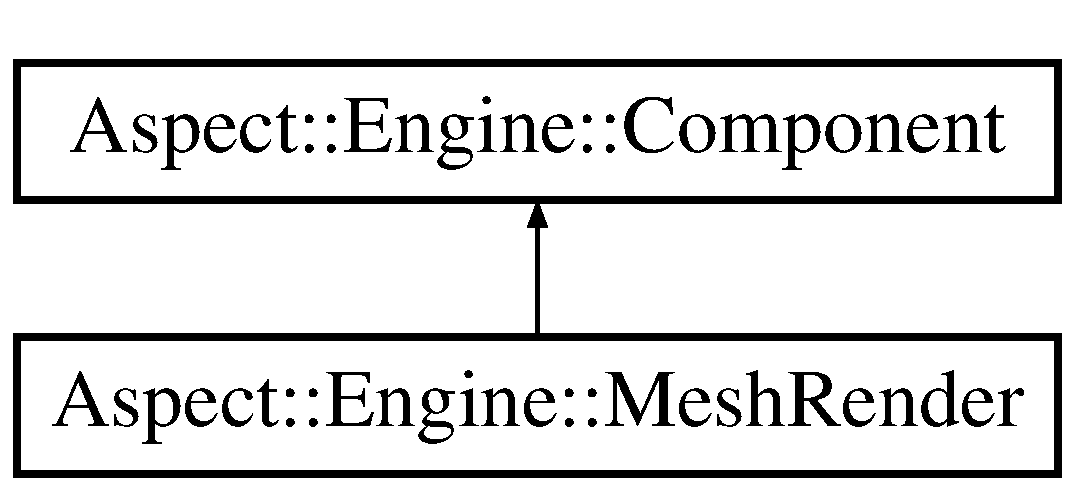
\includegraphics[height=2.000000cm]{class_aspect_1_1_engine_1_1_mesh_render}
\end{center}
\end{figure}
\subsection*{Public Member Functions}
\begin{DoxyCompactItemize}
\item 
\mbox{\hyperlink{_s_d_l__opengles2__gl2ext_8h_ae5d8fa23ad07c48bb609509eae494c95}{void}} \mbox{\hyperlink{class_aspect_1_1_engine_1_1_mesh_render_a54bb4394dafdc30e919a0ba5d9854871}{on\+Init}} ()
\item 
\mbox{\hyperlink{_s_d_l__opengles2__gl2ext_8h_ae5d8fa23ad07c48bb609509eae494c95}{void}} \mbox{\hyperlink{class_aspect_1_1_engine_1_1_mesh_render_a31478e2366177bf2e3c98fe71c769c33}{Cube}} ()
\item 
\mbox{\hyperlink{_s_d_l__opengles2__gl2ext_8h_ae5d8fa23ad07c48bb609509eae494c95}{void}} \mbox{\hyperlink{class_aspect_1_1_engine_1_1_mesh_render_ae8ca6b05b335b228943f4c034c02100d}{Triangle}} ()
\begin{DoxyCompactList}\small\item\em Draw cube object. \end{DoxyCompactList}\item 
\mbox{\hyperlink{_s_d_l__opengles2__gl2ext_8h_ae5d8fa23ad07c48bb609509eae494c95}{void}} \mbox{\hyperlink{class_aspect_1_1_engine_1_1_mesh_render_a16ef5a49a05bd542a33a78e67b4e3067}{Mesh}} (const \mbox{\hyperlink{_s_d_l__opengl__glext_8h_ae84541b4f3d8e1ea24ec0f466a8c568b}{std\+::string}} \&\+\_\+mesh)
\begin{DoxyCompactList}\small\item\em Draw Triangle. \end{DoxyCompactList}\item 
\mbox{\hyperlink{_s_d_l__opengles2__gl2ext_8h_ae5d8fa23ad07c48bb609509eae494c95}{void}} \mbox{\hyperlink{class_aspect_1_1_engine_1_1_mesh_render_aadfc13cdafe27ff3f63e80e68fdfbaa0}{set\+Texture}} (const \mbox{\hyperlink{_s_d_l__opengl__glext_8h_ae84541b4f3d8e1ea24ec0f466a8c568b}{std\+::string}} \&\+\_\+texture)
\begin{DoxyCompactList}\small\item\em Draw a mesh of any obj. \end{DoxyCompactList}\end{DoxyCompactItemize}
\subsection*{Public Attributes}
\begin{DoxyCompactItemize}
\item 
std\+::shared\+\_\+ptr$<$ \mbox{\hyperlink{class_aspect_1_1_engine_1_1_entity}{Entity}} $>$ \mbox{\hyperlink{class_aspect_1_1_engine_1_1_mesh_render_acd7bb5d1bfd42ecfe1a3d94b12271068}{camera}}
\begin{DoxyCompactList}\small\item\em On init component function. \end{DoxyCompactList}\item 
bool \mbox{\hyperlink{class_aspect_1_1_engine_1_1_mesh_render_a242e0980538e23b839f7ad8434bb1aa7}{Mr\+Enable}} = true
\end{DoxyCompactItemize}
\subsection*{Private Member Functions}
\begin{DoxyCompactItemize}
\item 
\mbox{\hyperlink{_s_d_l__opengles2__gl2ext_8h_ae5d8fa23ad07c48bb609509eae494c95}{void}} \mbox{\hyperlink{class_aspect_1_1_engine_1_1_mesh_render_aed81ecbd6bf1d63acb06171f729e4927}{on\+Display}} ()
\begin{DoxyCompactList}\small\item\em Set the texture of that model. \end{DoxyCompactList}\item 
\mbox{\hyperlink{_s_d_l__opengles2__gl2ext_8h_ae5d8fa23ad07c48bb609509eae494c95}{void}} \mbox{\hyperlink{class_aspect_1_1_engine_1_1_mesh_render_aebaa5a60d373d3363a13336cfbaa4141}{on\+Count}} ()
\begin{DoxyCompactList}\small\item\em On display works similar to draw function. \end{DoxyCompactList}\end{DoxyCompactItemize}
\subsection*{Private Attributes}
\begin{DoxyCompactItemize}
\item 
std\+::shared\+\_\+ptr$<$ \mbox{\hyperlink{class_aspect_1_1_engine_1_1_vertex_array}{Vertex\+Array}} $>$ \mbox{\hyperlink{class_aspect_1_1_engine_1_1_mesh_render_af137747f679a92eec890a25cbdbc9e8a}{shape}}
\begin{DoxyCompactList}\small\item\em On count is update. \end{DoxyCompactList}\item 
std\+::shared\+\_\+ptr$<$ \mbox{\hyperlink{class_aspect_1_1_engine_1_1_shader_program}{Shader\+Program}} $>$ \mbox{\hyperlink{class_aspect_1_1_engine_1_1_mesh_render_af49c803c0ee4b4e72e8d87455e74ae5e}{shader}}
\item 
std\+::shared\+\_\+ptr$<$ \mbox{\hyperlink{class_aspect_1_1_engine_1_1_material}{Material}} $>$ \mbox{\hyperlink{class_aspect_1_1_engine_1_1_mesh_render_ad1db374346473ead0d1c8c1801390dbe}{mat}}
\end{DoxyCompactItemize}


\subsection{Detailed Description}
Initialise Shader \mbox{\hyperlink{class_aspect_1_1_engine_1_1_program}{Program}}. 

\mbox{\hyperlink{class_aspect_1_1_engine_1_1_mesh_render}{Mesh\+Render}} is an inherited class of component 

\subsection{Member Function Documentation}
\mbox{\Hypertarget{class_aspect_1_1_engine_1_1_mesh_render_a31478e2366177bf2e3c98fe71c769c33}\label{class_aspect_1_1_engine_1_1_mesh_render_a31478e2366177bf2e3c98fe71c769c33}} 
\index{Aspect\+::\+Engine\+::\+Mesh\+Render@{Aspect\+::\+Engine\+::\+Mesh\+Render}!Cube@{Cube}}
\index{Cube@{Cube}!Aspect\+::\+Engine\+::\+Mesh\+Render@{Aspect\+::\+Engine\+::\+Mesh\+Render}}
\subsubsection{\texorpdfstring{Cube()}{Cube()}}
{\footnotesize\ttfamily \mbox{\hyperlink{_s_d_l__opengles2__gl2ext_8h_ae5d8fa23ad07c48bb609509eae494c95}{void}} Aspect\+::\+Engine\+::\+Mesh\+Render\+::\+Cube (\begin{DoxyParamCaption}{ }\end{DoxyParamCaption})}

\mbox{\Hypertarget{class_aspect_1_1_engine_1_1_mesh_render_a16ef5a49a05bd542a33a78e67b4e3067}\label{class_aspect_1_1_engine_1_1_mesh_render_a16ef5a49a05bd542a33a78e67b4e3067}} 
\index{Aspect\+::\+Engine\+::\+Mesh\+Render@{Aspect\+::\+Engine\+::\+Mesh\+Render}!Mesh@{Mesh}}
\index{Mesh@{Mesh}!Aspect\+::\+Engine\+::\+Mesh\+Render@{Aspect\+::\+Engine\+::\+Mesh\+Render}}
\subsubsection{\texorpdfstring{Mesh()}{Mesh()}}
{\footnotesize\ttfamily \mbox{\hyperlink{_s_d_l__opengles2__gl2ext_8h_ae5d8fa23ad07c48bb609509eae494c95}{void}} Aspect\+::\+Engine\+::\+Mesh\+Render\+::\+Mesh (\begin{DoxyParamCaption}\item[{const \mbox{\hyperlink{_s_d_l__opengl__glext_8h_ae84541b4f3d8e1ea24ec0f466a8c568b}{std\+::string}} \&}]{\+\_\+mesh }\end{DoxyParamCaption})}



Draw Triangle. 

\mbox{\Hypertarget{class_aspect_1_1_engine_1_1_mesh_render_aebaa5a60d373d3363a13336cfbaa4141}\label{class_aspect_1_1_engine_1_1_mesh_render_aebaa5a60d373d3363a13336cfbaa4141}} 
\index{Aspect\+::\+Engine\+::\+Mesh\+Render@{Aspect\+::\+Engine\+::\+Mesh\+Render}!on\+Count@{on\+Count}}
\index{on\+Count@{on\+Count}!Aspect\+::\+Engine\+::\+Mesh\+Render@{Aspect\+::\+Engine\+::\+Mesh\+Render}}
\subsubsection{\texorpdfstring{on\+Count()}{onCount()}}
{\footnotesize\ttfamily \mbox{\hyperlink{_s_d_l__opengles2__gl2ext_8h_ae5d8fa23ad07c48bb609509eae494c95}{void}} Aspect\+::\+Engine\+::\+Mesh\+Render\+::on\+Count (\begin{DoxyParamCaption}{ }\end{DoxyParamCaption})\hspace{0.3cm}{\ttfamily [private]}, {\ttfamily [virtual]}}



On display works similar to draw function. 



Reimplemented from \mbox{\hyperlink{class_aspect_1_1_engine_1_1_component_a02de673a0591459bd0d39e3022c1d3fc}{Aspect\+::\+Engine\+::\+Component}}.

\mbox{\Hypertarget{class_aspect_1_1_engine_1_1_mesh_render_aed81ecbd6bf1d63acb06171f729e4927}\label{class_aspect_1_1_engine_1_1_mesh_render_aed81ecbd6bf1d63acb06171f729e4927}} 
\index{Aspect\+::\+Engine\+::\+Mesh\+Render@{Aspect\+::\+Engine\+::\+Mesh\+Render}!on\+Display@{on\+Display}}
\index{on\+Display@{on\+Display}!Aspect\+::\+Engine\+::\+Mesh\+Render@{Aspect\+::\+Engine\+::\+Mesh\+Render}}
\subsubsection{\texorpdfstring{on\+Display()}{onDisplay()}}
{\footnotesize\ttfamily \mbox{\hyperlink{_s_d_l__opengles2__gl2ext_8h_ae5d8fa23ad07c48bb609509eae494c95}{void}} Aspect\+::\+Engine\+::\+Mesh\+Render\+::on\+Display (\begin{DoxyParamCaption}{ }\end{DoxyParamCaption})\hspace{0.3cm}{\ttfamily [private]}, {\ttfamily [virtual]}}



Set the texture of that model. 



Reimplemented from \mbox{\hyperlink{class_aspect_1_1_engine_1_1_component_ac67307dba854cdc9535a0de75e5a3d09}{Aspect\+::\+Engine\+::\+Component}}.

\mbox{\Hypertarget{class_aspect_1_1_engine_1_1_mesh_render_a54bb4394dafdc30e919a0ba5d9854871}\label{class_aspect_1_1_engine_1_1_mesh_render_a54bb4394dafdc30e919a0ba5d9854871}} 
\index{Aspect\+::\+Engine\+::\+Mesh\+Render@{Aspect\+::\+Engine\+::\+Mesh\+Render}!on\+Init@{on\+Init}}
\index{on\+Init@{on\+Init}!Aspect\+::\+Engine\+::\+Mesh\+Render@{Aspect\+::\+Engine\+::\+Mesh\+Render}}
\subsubsection{\texorpdfstring{on\+Init()}{onInit()}}
{\footnotesize\ttfamily \mbox{\hyperlink{_s_d_l__opengles2__gl2ext_8h_ae5d8fa23ad07c48bb609509eae494c95}{void}} Aspect\+::\+Engine\+::\+Mesh\+Render\+::on\+Init (\begin{DoxyParamCaption}{ }\end{DoxyParamCaption})\hspace{0.3cm}{\ttfamily [virtual]}}



Reimplemented from \mbox{\hyperlink{class_aspect_1_1_engine_1_1_component_a3a1fbf76e3fd208be7ffe0ffa449dcf9}{Aspect\+::\+Engine\+::\+Component}}.

\mbox{\Hypertarget{class_aspect_1_1_engine_1_1_mesh_render_aadfc13cdafe27ff3f63e80e68fdfbaa0}\label{class_aspect_1_1_engine_1_1_mesh_render_aadfc13cdafe27ff3f63e80e68fdfbaa0}} 
\index{Aspect\+::\+Engine\+::\+Mesh\+Render@{Aspect\+::\+Engine\+::\+Mesh\+Render}!set\+Texture@{set\+Texture}}
\index{set\+Texture@{set\+Texture}!Aspect\+::\+Engine\+::\+Mesh\+Render@{Aspect\+::\+Engine\+::\+Mesh\+Render}}
\subsubsection{\texorpdfstring{set\+Texture()}{setTexture()}}
{\footnotesize\ttfamily \mbox{\hyperlink{_s_d_l__opengles2__gl2ext_8h_ae5d8fa23ad07c48bb609509eae494c95}{void}} Aspect\+::\+Engine\+::\+Mesh\+Render\+::set\+Texture (\begin{DoxyParamCaption}\item[{const \mbox{\hyperlink{_s_d_l__opengl__glext_8h_ae84541b4f3d8e1ea24ec0f466a8c568b}{std\+::string}} \&}]{\+\_\+texture }\end{DoxyParamCaption})}



Draw a mesh of any obj. 

\mbox{\Hypertarget{class_aspect_1_1_engine_1_1_mesh_render_ae8ca6b05b335b228943f4c034c02100d}\label{class_aspect_1_1_engine_1_1_mesh_render_ae8ca6b05b335b228943f4c034c02100d}} 
\index{Aspect\+::\+Engine\+::\+Mesh\+Render@{Aspect\+::\+Engine\+::\+Mesh\+Render}!Triangle@{Triangle}}
\index{Triangle@{Triangle}!Aspect\+::\+Engine\+::\+Mesh\+Render@{Aspect\+::\+Engine\+::\+Mesh\+Render}}
\subsubsection{\texorpdfstring{Triangle()}{Triangle()}}
{\footnotesize\ttfamily \mbox{\hyperlink{_s_d_l__opengles2__gl2ext_8h_ae5d8fa23ad07c48bb609509eae494c95}{void}} Aspect\+::\+Engine\+::\+Mesh\+Render\+::\+Triangle (\begin{DoxyParamCaption}{ }\end{DoxyParamCaption})}



Draw cube object. 



\subsection{Member Data Documentation}
\mbox{\Hypertarget{class_aspect_1_1_engine_1_1_mesh_render_acd7bb5d1bfd42ecfe1a3d94b12271068}\label{class_aspect_1_1_engine_1_1_mesh_render_acd7bb5d1bfd42ecfe1a3d94b12271068}} 
\index{Aspect\+::\+Engine\+::\+Mesh\+Render@{Aspect\+::\+Engine\+::\+Mesh\+Render}!camera@{camera}}
\index{camera@{camera}!Aspect\+::\+Engine\+::\+Mesh\+Render@{Aspect\+::\+Engine\+::\+Mesh\+Render}}
\subsubsection{\texorpdfstring{camera}{camera}}
{\footnotesize\ttfamily std\+::shared\+\_\+ptr$<$\mbox{\hyperlink{class_aspect_1_1_engine_1_1_entity}{Entity}}$>$ Aspect\+::\+Engine\+::\+Mesh\+Render\+::camera}



On init component function. 

\mbox{\Hypertarget{class_aspect_1_1_engine_1_1_mesh_render_ad1db374346473ead0d1c8c1801390dbe}\label{class_aspect_1_1_engine_1_1_mesh_render_ad1db374346473ead0d1c8c1801390dbe}} 
\index{Aspect\+::\+Engine\+::\+Mesh\+Render@{Aspect\+::\+Engine\+::\+Mesh\+Render}!mat@{mat}}
\index{mat@{mat}!Aspect\+::\+Engine\+::\+Mesh\+Render@{Aspect\+::\+Engine\+::\+Mesh\+Render}}
\subsubsection{\texorpdfstring{mat}{mat}}
{\footnotesize\ttfamily std\+::shared\+\_\+ptr$<$\mbox{\hyperlink{class_aspect_1_1_engine_1_1_material}{Material}}$>$ Aspect\+::\+Engine\+::\+Mesh\+Render\+::mat\hspace{0.3cm}{\ttfamily [private]}}

\mbox{\Hypertarget{class_aspect_1_1_engine_1_1_mesh_render_a242e0980538e23b839f7ad8434bb1aa7}\label{class_aspect_1_1_engine_1_1_mesh_render_a242e0980538e23b839f7ad8434bb1aa7}} 
\index{Aspect\+::\+Engine\+::\+Mesh\+Render@{Aspect\+::\+Engine\+::\+Mesh\+Render}!Mr\+Enable@{Mr\+Enable}}
\index{Mr\+Enable@{Mr\+Enable}!Aspect\+::\+Engine\+::\+Mesh\+Render@{Aspect\+::\+Engine\+::\+Mesh\+Render}}
\subsubsection{\texorpdfstring{Mr\+Enable}{MrEnable}}
{\footnotesize\ttfamily bool Aspect\+::\+Engine\+::\+Mesh\+Render\+::\+Mr\+Enable = true}

\mbox{\Hypertarget{class_aspect_1_1_engine_1_1_mesh_render_af49c803c0ee4b4e72e8d87455e74ae5e}\label{class_aspect_1_1_engine_1_1_mesh_render_af49c803c0ee4b4e72e8d87455e74ae5e}} 
\index{Aspect\+::\+Engine\+::\+Mesh\+Render@{Aspect\+::\+Engine\+::\+Mesh\+Render}!shader@{shader}}
\index{shader@{shader}!Aspect\+::\+Engine\+::\+Mesh\+Render@{Aspect\+::\+Engine\+::\+Mesh\+Render}}
\subsubsection{\texorpdfstring{shader}{shader}}
{\footnotesize\ttfamily std\+::shared\+\_\+ptr$<$\mbox{\hyperlink{class_aspect_1_1_engine_1_1_shader_program}{Shader\+Program}}$>$ Aspect\+::\+Engine\+::\+Mesh\+Render\+::shader\hspace{0.3cm}{\ttfamily [private]}}

\mbox{\Hypertarget{class_aspect_1_1_engine_1_1_mesh_render_af137747f679a92eec890a25cbdbc9e8a}\label{class_aspect_1_1_engine_1_1_mesh_render_af137747f679a92eec890a25cbdbc9e8a}} 
\index{Aspect\+::\+Engine\+::\+Mesh\+Render@{Aspect\+::\+Engine\+::\+Mesh\+Render}!shape@{shape}}
\index{shape@{shape}!Aspect\+::\+Engine\+::\+Mesh\+Render@{Aspect\+::\+Engine\+::\+Mesh\+Render}}
\subsubsection{\texorpdfstring{shape}{shape}}
{\footnotesize\ttfamily std\+::shared\+\_\+ptr$<$\mbox{\hyperlink{class_aspect_1_1_engine_1_1_vertex_array}{Vertex\+Array}}$>$ Aspect\+::\+Engine\+::\+Mesh\+Render\+::shape\hspace{0.3cm}{\ttfamily [private]}}



On count is update. 



The documentation for this class was generated from the following files\+:\begin{DoxyCompactItemize}
\item 
src/\+Aspect/\mbox{\hyperlink{_mesh_render_8h}{Mesh\+Render.\+h}}\item 
src/\+Aspect/\mbox{\hyperlink{_mesh_render_8cpp}{Mesh\+Render.\+cpp}}\end{DoxyCompactItemize}

\hypertarget{class_aspect_1_1_engine_1_1_program}{}\section{Aspect\+:\+:Engine\+:\+:Program Class Reference}
\label{class_aspect_1_1_engine_1_1_program}\index{Aspect\+::\+Engine\+::\+Program@{Aspect\+::\+Engine\+::\+Program}}


\mbox{\hyperlink{class_aspect_1_1_engine_1_1_program}{Program}} class the main class that oganises the program.  




{\ttfamily \#include $<$Program.\+h$>$}

\subsection*{Public Member Functions}
\begin{DoxyCompactItemize}
\item 
\mbox{\hyperlink{_s_d_l__opengles2__gl2ext_8h_ae5d8fa23ad07c48bb609509eae494c95}{void}} \mbox{\hyperlink{class_aspect_1_1_engine_1_1_program_acd8c11ab08516997e18bc97412cb65cc}{Start}} (std\+::shared\+\_\+ptr$<$ \mbox{\hyperlink{class_aspect_1_1_engine_1_1_entity}{Entity}} $>$ \+\_\+cam, std\+::shared\+\_\+ptr$<$ \mbox{\hyperlink{class_aspect_1_1_engine_1_1_entity}{Entity}} $>$ \+\_\+player)
\item 
\mbox{\hyperlink{_s_d_l__opengles2__gl2ext_8h_ae5d8fa23ad07c48bb609509eae494c95}{void}} \mbox{\hyperlink{class_aspect_1_1_engine_1_1_program_aebf5093c9edb094862fc4fa0823d87e5}{End}} ()
\begin{DoxyCompactList}\small\item\em Start the program, also contains the game loop. \end{DoxyCompactList}\item 
\mbox{\hyperlink{_s_d_l__opengles2__gl2ext_8h_ae5d8fa23ad07c48bb609509eae494c95}{void}} \mbox{\hyperlink{class_aspect_1_1_engine_1_1_program_a2226e1a84c31b158c05492c9db9de1a2}{set\+Current\+Camera}} (std\+::shared\+\_\+ptr$<$ \mbox{\hyperlink{class_aspect_1_1_engine_1_1_camera}{Camera}} $>$ cam)
\begin{DoxyCompactList}\small\item\em Add entity function. \end{DoxyCompactList}\item 
std\+::shared\+\_\+ptr$<$ \mbox{\hyperlink{class_aspect_1_1_engine_1_1_camera}{Camera}} $>$ \mbox{\hyperlink{class_aspect_1_1_engine_1_1_program_a44f49997a17637fdc60a890c44f74eca}{get\+Current\+Camera}} ()
\begin{DoxyCompactList}\small\item\em Set the current camera. \end{DoxyCompactList}\end{DoxyCompactItemize}
\subsection*{Static Public Member Functions}
\begin{DoxyCompactItemize}
\item 
static bool \mbox{\hyperlink{class_aspect_1_1_engine_1_1_program_ad43c625aadbe66c58cf2c89f3aea0b67}{Init\+Glew}} ()
\begin{DoxyCompactList}\small\item\em Clean up and close the program. \end{DoxyCompactList}\item 
static std\+::shared\+\_\+ptr$<$ \mbox{\hyperlink{class_aspect_1_1_engine_1_1_program}{Program}} $>$ \mbox{\hyperlink{class_aspect_1_1_engine_1_1_program_a0defbfe96a9811ed16b1d02d786caba0}{Init\+S\+DL}} ()
\begin{DoxyCompactList}\small\item\em Initialise Glew. \end{DoxyCompactList}\item 
static std\+::shared\+\_\+ptr$<$ \mbox{\hyperlink{class_aspect_1_1_engine_1_1_entity}{Entity}} $>$ \mbox{\hyperlink{class_aspect_1_1_engine_1_1_program_a937df3d57a425f25be2f40c3dcaff072}{add\+Entity}} ()
\begin{DoxyCompactList}\small\item\em Initialise S\+DL. \end{DoxyCompactList}\end{DoxyCompactItemize}
\subsection*{Public Attributes}
\begin{DoxyCompactItemize}
\item 
float \mbox{\hyperlink{class_aspect_1_1_engine_1_1_program_ab387e4928975cfedaa081f8fc7b61bc1}{last\+CubeX}} = -\/6.\+0f
\begin{DoxyCompactList}\small\item\em Get the location and martix of the current camera. \end{DoxyCompactList}\item 
float \mbox{\hyperlink{class_aspect_1_1_engine_1_1_program_ad2cae5125b23074393f6ad5681a24fa0}{RandomX}} = -\/10.\+0f
\item 
float \mbox{\hyperlink{class_aspect_1_1_engine_1_1_program_a5779fcff2573e7c5e92878c964f5a701}{backgroundX}} = -\/10.\+0f
\item 
bool \mbox{\hyperlink{class_aspect_1_1_engine_1_1_program_a76e0a879e2a03987fc7242275d311579}{running}}
\end{DoxyCompactItemize}
\subsection*{Static Protected Attributes}
\begin{DoxyCompactItemize}
\item 
static \mbox{\hyperlink{group__core__types_ga7dcd2365c2e368e6af5b7adeb6a9c8df}{glm\+::mat4}} \mbox{\hyperlink{class_aspect_1_1_engine_1_1_program_a713b2d1d51158b44ffcc97f7f69933a4}{model\+Matrix}}
\end{DoxyCompactItemize}
\subsection*{Private Attributes}
\begin{DoxyCompactItemize}
\item 
\mbox{\hyperlink{alc_8h_aba8742179fd52ef41c66adacdec5383e}{A\+L\+Cdevice}} $\ast$ \mbox{\hyperlink{class_aspect_1_1_engine_1_1_program_aa4689537736d1273e4e644947a61c465}{device}}
\item 
\mbox{\hyperlink{alc_8h_ad085cf94ff96646b5a2b5401c4489e23}{A\+L\+Ccontext}} $\ast$ \mbox{\hyperlink{class_aspect_1_1_engine_1_1_program_ac5c7dbe0c0a08b0603625567e08e5c46}{context}}
\item 
std\+::weak\+\_\+ptr$<$ \mbox{\hyperlink{class_aspect_1_1_engine_1_1_camera}{Camera}} $>$ \mbox{\hyperlink{class_aspect_1_1_engine_1_1_program_ab013b5b5fc5de055ccbb70d44b49de8a}{current\+Cam}}
\end{DoxyCompactItemize}
\subsection*{Static Private Attributes}
\begin{DoxyCompactItemize}
\item 
static std\+::vector$<$ std\+::shared\+\_\+ptr$<$ \mbox{\hyperlink{class_aspect_1_1_engine_1_1_entity}{Entity}} $>$ $>$ \mbox{\hyperlink{class_aspect_1_1_engine_1_1_program_a553a6feb2e63f3901ddfad5ebba9fa99}{entities}}
\item 
static std\+::weak\+\_\+ptr$<$ \mbox{\hyperlink{class_aspect_1_1_engine_1_1_program}{Program}} $>$ \mbox{\hyperlink{class_aspect_1_1_engine_1_1_program_a956d0f100139d714030fa5449c2c2849}{self}}
\item 
static \mbox{\hyperlink{_s_d_l__video_8h_a55a196c7d3b8497538632c79ae1e6392}{S\+D\+L\+\_\+\+Window}} $\ast$ \mbox{\hyperlink{class_aspect_1_1_engine_1_1_program_a674502c50c3ab53a86dd2d7966b2506d}{\+\_\+window}}
\end{DoxyCompactItemize}


\subsection{Detailed Description}
\mbox{\hyperlink{class_aspect_1_1_engine_1_1_program}{Program}} class the main class that oganises the program. 

\subsection{Member Function Documentation}
\mbox{\Hypertarget{class_aspect_1_1_engine_1_1_program_a937df3d57a425f25be2f40c3dcaff072}\label{class_aspect_1_1_engine_1_1_program_a937df3d57a425f25be2f40c3dcaff072}} 
\index{Aspect\+::\+Engine\+::\+Program@{Aspect\+::\+Engine\+::\+Program}!add\+Entity@{add\+Entity}}
\index{add\+Entity@{add\+Entity}!Aspect\+::\+Engine\+::\+Program@{Aspect\+::\+Engine\+::\+Program}}
\subsubsection{\texorpdfstring{add\+Entity()}{addEntity()}}
{\footnotesize\ttfamily std\+::shared\+\_\+ptr$<$ \mbox{\hyperlink{class_aspect_1_1_engine_1_1_entity}{Entity}} $>$ Aspect\+::\+Engine\+::\+Program\+::add\+Entity (\begin{DoxyParamCaption}{ }\end{DoxyParamCaption})\hspace{0.3cm}{\ttfamily [static]}}



Initialise S\+DL. 

\mbox{\Hypertarget{class_aspect_1_1_engine_1_1_program_aebf5093c9edb094862fc4fa0823d87e5}\label{class_aspect_1_1_engine_1_1_program_aebf5093c9edb094862fc4fa0823d87e5}} 
\index{Aspect\+::\+Engine\+::\+Program@{Aspect\+::\+Engine\+::\+Program}!End@{End}}
\index{End@{End}!Aspect\+::\+Engine\+::\+Program@{Aspect\+::\+Engine\+::\+Program}}
\subsubsection{\texorpdfstring{End()}{End()}}
{\footnotesize\ttfamily \mbox{\hyperlink{_s_d_l__opengles2__gl2ext_8h_ae5d8fa23ad07c48bb609509eae494c95}{void}} Aspect\+::\+Engine\+::\+Program\+::\+End (\begin{DoxyParamCaption}{ }\end{DoxyParamCaption})}



Start the program, also contains the game loop. 

\mbox{\Hypertarget{class_aspect_1_1_engine_1_1_program_a44f49997a17637fdc60a890c44f74eca}\label{class_aspect_1_1_engine_1_1_program_a44f49997a17637fdc60a890c44f74eca}} 
\index{Aspect\+::\+Engine\+::\+Program@{Aspect\+::\+Engine\+::\+Program}!get\+Current\+Camera@{get\+Current\+Camera}}
\index{get\+Current\+Camera@{get\+Current\+Camera}!Aspect\+::\+Engine\+::\+Program@{Aspect\+::\+Engine\+::\+Program}}
\subsubsection{\texorpdfstring{get\+Current\+Camera()}{getCurrentCamera()}}
{\footnotesize\ttfamily std\+::shared\+\_\+ptr$<$ \mbox{\hyperlink{class_aspect_1_1_engine_1_1_camera}{Camera}} $>$ Aspect\+::\+Engine\+::\+Program\+::get\+Current\+Camera (\begin{DoxyParamCaption}{ }\end{DoxyParamCaption})}



Set the current camera. 

\mbox{\Hypertarget{class_aspect_1_1_engine_1_1_program_ad43c625aadbe66c58cf2c89f3aea0b67}\label{class_aspect_1_1_engine_1_1_program_ad43c625aadbe66c58cf2c89f3aea0b67}} 
\index{Aspect\+::\+Engine\+::\+Program@{Aspect\+::\+Engine\+::\+Program}!Init\+Glew@{Init\+Glew}}
\index{Init\+Glew@{Init\+Glew}!Aspect\+::\+Engine\+::\+Program@{Aspect\+::\+Engine\+::\+Program}}
\subsubsection{\texorpdfstring{Init\+Glew()}{InitGlew()}}
{\footnotesize\ttfamily bool Aspect\+::\+Engine\+::\+Program\+::\+Init\+Glew (\begin{DoxyParamCaption}{ }\end{DoxyParamCaption})\hspace{0.3cm}{\ttfamily [static]}}



Clean up and close the program. 

\mbox{\Hypertarget{class_aspect_1_1_engine_1_1_program_a0defbfe96a9811ed16b1d02d786caba0}\label{class_aspect_1_1_engine_1_1_program_a0defbfe96a9811ed16b1d02d786caba0}} 
\index{Aspect\+::\+Engine\+::\+Program@{Aspect\+::\+Engine\+::\+Program}!Init\+S\+DL@{Init\+S\+DL}}
\index{Init\+S\+DL@{Init\+S\+DL}!Aspect\+::\+Engine\+::\+Program@{Aspect\+::\+Engine\+::\+Program}}
\subsubsection{\texorpdfstring{Init\+S\+D\+L()}{InitSDL()}}
{\footnotesize\ttfamily std\+::shared\+\_\+ptr$<$ \mbox{\hyperlink{class_aspect_1_1_engine_1_1_program}{Program}} $>$ Aspect\+::\+Engine\+::\+Program\+::\+Init\+S\+DL (\begin{DoxyParamCaption}{ }\end{DoxyParamCaption})\hspace{0.3cm}{\ttfamily [static]}}



Initialise Glew. 

\mbox{\Hypertarget{class_aspect_1_1_engine_1_1_program_a2226e1a84c31b158c05492c9db9de1a2}\label{class_aspect_1_1_engine_1_1_program_a2226e1a84c31b158c05492c9db9de1a2}} 
\index{Aspect\+::\+Engine\+::\+Program@{Aspect\+::\+Engine\+::\+Program}!set\+Current\+Camera@{set\+Current\+Camera}}
\index{set\+Current\+Camera@{set\+Current\+Camera}!Aspect\+::\+Engine\+::\+Program@{Aspect\+::\+Engine\+::\+Program}}
\subsubsection{\texorpdfstring{set\+Current\+Camera()}{setCurrentCamera()}}
{\footnotesize\ttfamily \mbox{\hyperlink{_s_d_l__opengles2__gl2ext_8h_ae5d8fa23ad07c48bb609509eae494c95}{void}} Aspect\+::\+Engine\+::\+Program\+::set\+Current\+Camera (\begin{DoxyParamCaption}\item[{std\+::shared\+\_\+ptr$<$ \mbox{\hyperlink{class_aspect_1_1_engine_1_1_camera}{Camera}} $>$}]{cam }\end{DoxyParamCaption})}



Add entity function. 

\mbox{\Hypertarget{class_aspect_1_1_engine_1_1_program_acd8c11ab08516997e18bc97412cb65cc}\label{class_aspect_1_1_engine_1_1_program_acd8c11ab08516997e18bc97412cb65cc}} 
\index{Aspect\+::\+Engine\+::\+Program@{Aspect\+::\+Engine\+::\+Program}!Start@{Start}}
\index{Start@{Start}!Aspect\+::\+Engine\+::\+Program@{Aspect\+::\+Engine\+::\+Program}}
\subsubsection{\texorpdfstring{Start()}{Start()}}
{\footnotesize\ttfamily \mbox{\hyperlink{_s_d_l__opengles2__gl2ext_8h_ae5d8fa23ad07c48bb609509eae494c95}{void}} Aspect\+::\+Engine\+::\+Program\+::\+Start (\begin{DoxyParamCaption}\item[{std\+::shared\+\_\+ptr$<$ \mbox{\hyperlink{class_aspect_1_1_engine_1_1_entity}{Entity}} $>$}]{\+\_\+cam,  }\item[{std\+::shared\+\_\+ptr$<$ \mbox{\hyperlink{class_aspect_1_1_engine_1_1_entity}{Entity}} $>$}]{\+\_\+player }\end{DoxyParamCaption})}



\subsection{Member Data Documentation}
\mbox{\Hypertarget{class_aspect_1_1_engine_1_1_program_a674502c50c3ab53a86dd2d7966b2506d}\label{class_aspect_1_1_engine_1_1_program_a674502c50c3ab53a86dd2d7966b2506d}} 
\index{Aspect\+::\+Engine\+::\+Program@{Aspect\+::\+Engine\+::\+Program}!\+\_\+window@{\+\_\+window}}
\index{\+\_\+window@{\+\_\+window}!Aspect\+::\+Engine\+::\+Program@{Aspect\+::\+Engine\+::\+Program}}
\subsubsection{\texorpdfstring{\+\_\+window}{\_window}}
{\footnotesize\ttfamily \mbox{\hyperlink{_s_d_l__video_8h_a55a196c7d3b8497538632c79ae1e6392}{S\+D\+L\+\_\+\+Window}} $\ast$ Aspect\+::\+Engine\+::\+Program\+::\+\_\+window\hspace{0.3cm}{\ttfamily [static]}, {\ttfamily [private]}}

\mbox{\Hypertarget{class_aspect_1_1_engine_1_1_program_a5779fcff2573e7c5e92878c964f5a701}\label{class_aspect_1_1_engine_1_1_program_a5779fcff2573e7c5e92878c964f5a701}} 
\index{Aspect\+::\+Engine\+::\+Program@{Aspect\+::\+Engine\+::\+Program}!backgroundX@{backgroundX}}
\index{backgroundX@{backgroundX}!Aspect\+::\+Engine\+::\+Program@{Aspect\+::\+Engine\+::\+Program}}
\subsubsection{\texorpdfstring{backgroundX}{backgroundX}}
{\footnotesize\ttfamily float Aspect\+::\+Engine\+::\+Program\+::backgroundX = -\/10.\+0f}

\mbox{\Hypertarget{class_aspect_1_1_engine_1_1_program_ac5c7dbe0c0a08b0603625567e08e5c46}\label{class_aspect_1_1_engine_1_1_program_ac5c7dbe0c0a08b0603625567e08e5c46}} 
\index{Aspect\+::\+Engine\+::\+Program@{Aspect\+::\+Engine\+::\+Program}!context@{context}}
\index{context@{context}!Aspect\+::\+Engine\+::\+Program@{Aspect\+::\+Engine\+::\+Program}}
\subsubsection{\texorpdfstring{context}{context}}
{\footnotesize\ttfamily \mbox{\hyperlink{alc_8h_ad085cf94ff96646b5a2b5401c4489e23}{A\+L\+Ccontext}}$\ast$ Aspect\+::\+Engine\+::\+Program\+::context\hspace{0.3cm}{\ttfamily [private]}}

\mbox{\Hypertarget{class_aspect_1_1_engine_1_1_program_ab013b5b5fc5de055ccbb70d44b49de8a}\label{class_aspect_1_1_engine_1_1_program_ab013b5b5fc5de055ccbb70d44b49de8a}} 
\index{Aspect\+::\+Engine\+::\+Program@{Aspect\+::\+Engine\+::\+Program}!current\+Cam@{current\+Cam}}
\index{current\+Cam@{current\+Cam}!Aspect\+::\+Engine\+::\+Program@{Aspect\+::\+Engine\+::\+Program}}
\subsubsection{\texorpdfstring{current\+Cam}{currentCam}}
{\footnotesize\ttfamily std\+::weak\+\_\+ptr$<$\mbox{\hyperlink{class_aspect_1_1_engine_1_1_camera}{Camera}}$>$ Aspect\+::\+Engine\+::\+Program\+::current\+Cam\hspace{0.3cm}{\ttfamily [private]}}

\mbox{\Hypertarget{class_aspect_1_1_engine_1_1_program_aa4689537736d1273e4e644947a61c465}\label{class_aspect_1_1_engine_1_1_program_aa4689537736d1273e4e644947a61c465}} 
\index{Aspect\+::\+Engine\+::\+Program@{Aspect\+::\+Engine\+::\+Program}!device@{device}}
\index{device@{device}!Aspect\+::\+Engine\+::\+Program@{Aspect\+::\+Engine\+::\+Program}}
\subsubsection{\texorpdfstring{device}{device}}
{\footnotesize\ttfamily \mbox{\hyperlink{alc_8h_aba8742179fd52ef41c66adacdec5383e}{A\+L\+Cdevice}}$\ast$ Aspect\+::\+Engine\+::\+Program\+::device\hspace{0.3cm}{\ttfamily [private]}}

\mbox{\Hypertarget{class_aspect_1_1_engine_1_1_program_a553a6feb2e63f3901ddfad5ebba9fa99}\label{class_aspect_1_1_engine_1_1_program_a553a6feb2e63f3901ddfad5ebba9fa99}} 
\index{Aspect\+::\+Engine\+::\+Program@{Aspect\+::\+Engine\+::\+Program}!entities@{entities}}
\index{entities@{entities}!Aspect\+::\+Engine\+::\+Program@{Aspect\+::\+Engine\+::\+Program}}
\subsubsection{\texorpdfstring{entities}{entities}}
{\footnotesize\ttfamily std\+::vector$<$ std\+::shared\+\_\+ptr$<$ \mbox{\hyperlink{class_aspect_1_1_engine_1_1_entity}{Entity}} $>$ $>$ Aspect\+::\+Engine\+::\+Program\+::entities\hspace{0.3cm}{\ttfamily [static]}, {\ttfamily [private]}}

\mbox{\Hypertarget{class_aspect_1_1_engine_1_1_program_ab387e4928975cfedaa081f8fc7b61bc1}\label{class_aspect_1_1_engine_1_1_program_ab387e4928975cfedaa081f8fc7b61bc1}} 
\index{Aspect\+::\+Engine\+::\+Program@{Aspect\+::\+Engine\+::\+Program}!last\+CubeX@{last\+CubeX}}
\index{last\+CubeX@{last\+CubeX}!Aspect\+::\+Engine\+::\+Program@{Aspect\+::\+Engine\+::\+Program}}
\subsubsection{\texorpdfstring{last\+CubeX}{lastCubeX}}
{\footnotesize\ttfamily float Aspect\+::\+Engine\+::\+Program\+::last\+CubeX = -\/6.\+0f}



Get the location and martix of the current camera. 

\mbox{\Hypertarget{class_aspect_1_1_engine_1_1_program_a713b2d1d51158b44ffcc97f7f69933a4}\label{class_aspect_1_1_engine_1_1_program_a713b2d1d51158b44ffcc97f7f69933a4}} 
\index{Aspect\+::\+Engine\+::\+Program@{Aspect\+::\+Engine\+::\+Program}!model\+Matrix@{model\+Matrix}}
\index{model\+Matrix@{model\+Matrix}!Aspect\+::\+Engine\+::\+Program@{Aspect\+::\+Engine\+::\+Program}}
\subsubsection{\texorpdfstring{model\+Matrix}{modelMatrix}}
{\footnotesize\ttfamily \mbox{\hyperlink{group__core__types_ga7dcd2365c2e368e6af5b7adeb6a9c8df}{glm\+::mat4}} Aspect\+::\+Engine\+::\+Program\+::model\+Matrix\hspace{0.3cm}{\ttfamily [static]}, {\ttfamily [protected]}}

\mbox{\Hypertarget{class_aspect_1_1_engine_1_1_program_ad2cae5125b23074393f6ad5681a24fa0}\label{class_aspect_1_1_engine_1_1_program_ad2cae5125b23074393f6ad5681a24fa0}} 
\index{Aspect\+::\+Engine\+::\+Program@{Aspect\+::\+Engine\+::\+Program}!RandomX@{RandomX}}
\index{RandomX@{RandomX}!Aspect\+::\+Engine\+::\+Program@{Aspect\+::\+Engine\+::\+Program}}
\subsubsection{\texorpdfstring{RandomX}{RandomX}}
{\footnotesize\ttfamily float Aspect\+::\+Engine\+::\+Program\+::\+RandomX = -\/10.\+0f}

\mbox{\Hypertarget{class_aspect_1_1_engine_1_1_program_a76e0a879e2a03987fc7242275d311579}\label{class_aspect_1_1_engine_1_1_program_a76e0a879e2a03987fc7242275d311579}} 
\index{Aspect\+::\+Engine\+::\+Program@{Aspect\+::\+Engine\+::\+Program}!running@{running}}
\index{running@{running}!Aspect\+::\+Engine\+::\+Program@{Aspect\+::\+Engine\+::\+Program}}
\subsubsection{\texorpdfstring{running}{running}}
{\footnotesize\ttfamily bool Aspect\+::\+Engine\+::\+Program\+::running}

\mbox{\Hypertarget{class_aspect_1_1_engine_1_1_program_a956d0f100139d714030fa5449c2c2849}\label{class_aspect_1_1_engine_1_1_program_a956d0f100139d714030fa5449c2c2849}} 
\index{Aspect\+::\+Engine\+::\+Program@{Aspect\+::\+Engine\+::\+Program}!self@{self}}
\index{self@{self}!Aspect\+::\+Engine\+::\+Program@{Aspect\+::\+Engine\+::\+Program}}
\subsubsection{\texorpdfstring{self}{self}}
{\footnotesize\ttfamily std\+::weak\+\_\+ptr$<$ \mbox{\hyperlink{class_aspect_1_1_engine_1_1_program}{Program}} $>$ Aspect\+::\+Engine\+::\+Program\+::self\hspace{0.3cm}{\ttfamily [static]}, {\ttfamily [private]}}



The documentation for this class was generated from the following files\+:\begin{DoxyCompactItemize}
\item 
src/\+Aspect/\mbox{\hyperlink{_program_8h}{Program.\+h}}\item 
src/\+Aspect/\mbox{\hyperlink{_program_8cpp}{Program.\+cpp}}\end{DoxyCompactItemize}

\hypertarget{struct_aspect_1_1_engine_1_1_sampler}{}\section{Aspect\+:\+:Engine\+:\+:Sampler Struct Reference}
\label{struct_aspect_1_1_engine_1_1_sampler}\index{Aspect\+::\+Engine\+::\+Sampler@{Aspect\+::\+Engine\+::\+Sampler}}


Initialise \mbox{\hyperlink{class_aspect_1_1_engine_1_1_material}{Material}} class.  




{\ttfamily \#include $<$Shader\+Program.\+h$>$}

\subsection*{Public Attributes}
\begin{DoxyCompactItemize}
\item 
\mbox{\hyperlink{glew_8h_acebcc1c5663f14ebde1d16831e5fed94}{G\+Lint}} \mbox{\hyperlink{struct_aspect_1_1_engine_1_1_sampler_a8b331dd0334126edee31cfa525101b66}{id}}
\item 
std\+::shared\+\_\+ptr$<$ \mbox{\hyperlink{class_aspect_1_1_engine_1_1_material}{Material}} $>$ \mbox{\hyperlink{struct_aspect_1_1_engine_1_1_sampler_acab2c584b4973154fe061a8398867de4}{mat}}
\end{DoxyCompactItemize}


\subsection{Detailed Description}
Initialise \mbox{\hyperlink{class_aspect_1_1_engine_1_1_material}{Material}} class. 

Struct for the material sample 

\subsection{Member Data Documentation}
\mbox{\Hypertarget{struct_aspect_1_1_engine_1_1_sampler_a8b331dd0334126edee31cfa525101b66}\label{struct_aspect_1_1_engine_1_1_sampler_a8b331dd0334126edee31cfa525101b66}} 
\index{Aspect\+::\+Engine\+::\+Sampler@{Aspect\+::\+Engine\+::\+Sampler}!id@{id}}
\index{id@{id}!Aspect\+::\+Engine\+::\+Sampler@{Aspect\+::\+Engine\+::\+Sampler}}
\subsubsection{\texorpdfstring{id}{id}}
{\footnotesize\ttfamily \mbox{\hyperlink{glew_8h_acebcc1c5663f14ebde1d16831e5fed94}{G\+Lint}} Aspect\+::\+Engine\+::\+Sampler\+::id}

\mbox{\Hypertarget{struct_aspect_1_1_engine_1_1_sampler_acab2c584b4973154fe061a8398867de4}\label{struct_aspect_1_1_engine_1_1_sampler_acab2c584b4973154fe061a8398867de4}} 
\index{Aspect\+::\+Engine\+::\+Sampler@{Aspect\+::\+Engine\+::\+Sampler}!mat@{mat}}
\index{mat@{mat}!Aspect\+::\+Engine\+::\+Sampler@{Aspect\+::\+Engine\+::\+Sampler}}
\subsubsection{\texorpdfstring{mat}{mat}}
{\footnotesize\ttfamily std\+::shared\+\_\+ptr$<$\mbox{\hyperlink{class_aspect_1_1_engine_1_1_material}{Material}}$>$ Aspect\+::\+Engine\+::\+Sampler\+::mat}



The documentation for this struct was generated from the following file\+:\begin{DoxyCompactItemize}
\item 
src/\+Aspect/\mbox{\hyperlink{_shader_program_8h}{Shader\+Program.\+h}}\end{DoxyCompactItemize}

\hypertarget{class_aspect_1_1_engine_1_1_shader_program}{}\section{Aspect\+:\+:Engine\+:\+:Shader\+Program Class Reference}
\label{class_aspect_1_1_engine_1_1_shader_program}\index{Aspect\+::\+Engine\+::\+Shader\+Program@{Aspect\+::\+Engine\+::\+Shader\+Program}}


{\ttfamily \#include $<$Shader\+Program.\+h$>$}

\subsection*{Public Member Functions}
\begin{DoxyCompactItemize}
\item 
\mbox{\hyperlink{class_aspect_1_1_engine_1_1_shader_program_acfd947e0ce600660979f192b80fb41ea}{Shader\+Program}} (std\+::string vert, std\+::string frag)
\item 
void \mbox{\hyperlink{class_aspect_1_1_engine_1_1_shader_program_a4ecfbdda05fbfb1d5a36f6d584dd0ef2}{draw}} (std\+::shared\+\_\+ptr$<$ \mbox{\hyperlink{class_aspect_1_1_engine_1_1_vertex_array}{Vertex\+Array}} $>$ v\+Array)
\item 
void \mbox{\hyperlink{class_aspect_1_1_engine_1_1_shader_program_aefda3028d33a268999baca3a953d0ac8}{set\+Uniform}} (std\+::string uniform, glm\+::vec4 value)
\item 
void \mbox{\hyperlink{class_aspect_1_1_engine_1_1_shader_program_ac294314ed82949d84ad00deeffba56bd}{set\+Uniform}} (std\+::string uniform, float value)
\item 
void \mbox{\hyperlink{class_aspect_1_1_engine_1_1_shader_program_a9ed3540c0a42dd353b4c18b3df99d279}{set\+Uniform}} (std\+::string uniform, glm\+::mat4 value)
\item 
void \mbox{\hyperlink{class_aspect_1_1_engine_1_1_shader_program_abfaf605b8dfade33b086b2f33e07762b}{set\+Uniform}} (std\+::string uniform, std\+::shared\+\_\+ptr$<$ \mbox{\hyperlink{class_aspect_1_1_engine_1_1_material}{Material}} $>$ mat)
\item 
G\+Luint \mbox{\hyperlink{class_aspect_1_1_engine_1_1_shader_program_a78a54e4a39c3e605f7a5832e6ce7f692}{get\+Id}} ()
\end{DoxyCompactItemize}


\subsection{Constructor \& Destructor Documentation}
\mbox{\Hypertarget{class_aspect_1_1_engine_1_1_shader_program_acfd947e0ce600660979f192b80fb41ea}\label{class_aspect_1_1_engine_1_1_shader_program_acfd947e0ce600660979f192b80fb41ea}} 
\index{Aspect\+::\+Engine\+::\+Shader\+Program@{Aspect\+::\+Engine\+::\+Shader\+Program}!Shader\+Program@{Shader\+Program}}
\index{Shader\+Program@{Shader\+Program}!Aspect\+::\+Engine\+::\+Shader\+Program@{Aspect\+::\+Engine\+::\+Shader\+Program}}
\subsubsection{\texorpdfstring{Shader\+Program()}{ShaderProgram()}}
{\footnotesize\ttfamily Aspect\+::\+Engine\+::\+Shader\+Program\+::\+Shader\+Program (\begin{DoxyParamCaption}\item[{std\+::string}]{vert,  }\item[{std\+::string}]{frag }\end{DoxyParamCaption})}



\subsection{Member Function Documentation}
\mbox{\Hypertarget{class_aspect_1_1_engine_1_1_shader_program_a4ecfbdda05fbfb1d5a36f6d584dd0ef2}\label{class_aspect_1_1_engine_1_1_shader_program_a4ecfbdda05fbfb1d5a36f6d584dd0ef2}} 
\index{Aspect\+::\+Engine\+::\+Shader\+Program@{Aspect\+::\+Engine\+::\+Shader\+Program}!draw@{draw}}
\index{draw@{draw}!Aspect\+::\+Engine\+::\+Shader\+Program@{Aspect\+::\+Engine\+::\+Shader\+Program}}
\subsubsection{\texorpdfstring{draw()}{draw()}}
{\footnotesize\ttfamily void Aspect\+::\+Engine\+::\+Shader\+Program\+::draw (\begin{DoxyParamCaption}\item[{std\+::shared\+\_\+ptr$<$ \mbox{\hyperlink{class_aspect_1_1_engine_1_1_vertex_array}{Vertex\+Array}} $>$}]{v\+Array }\end{DoxyParamCaption})}

\mbox{\Hypertarget{class_aspect_1_1_engine_1_1_shader_program_a78a54e4a39c3e605f7a5832e6ce7f692}\label{class_aspect_1_1_engine_1_1_shader_program_a78a54e4a39c3e605f7a5832e6ce7f692}} 
\index{Aspect\+::\+Engine\+::\+Shader\+Program@{Aspect\+::\+Engine\+::\+Shader\+Program}!get\+Id@{get\+Id}}
\index{get\+Id@{get\+Id}!Aspect\+::\+Engine\+::\+Shader\+Program@{Aspect\+::\+Engine\+::\+Shader\+Program}}
\subsubsection{\texorpdfstring{get\+Id()}{getId()}}
{\footnotesize\ttfamily G\+Luint Aspect\+::\+Engine\+::\+Shader\+Program\+::get\+Id (\begin{DoxyParamCaption}{ }\end{DoxyParamCaption})}

\mbox{\Hypertarget{class_aspect_1_1_engine_1_1_shader_program_aefda3028d33a268999baca3a953d0ac8}\label{class_aspect_1_1_engine_1_1_shader_program_aefda3028d33a268999baca3a953d0ac8}} 
\index{Aspect\+::\+Engine\+::\+Shader\+Program@{Aspect\+::\+Engine\+::\+Shader\+Program}!set\+Uniform@{set\+Uniform}}
\index{set\+Uniform@{set\+Uniform}!Aspect\+::\+Engine\+::\+Shader\+Program@{Aspect\+::\+Engine\+::\+Shader\+Program}}
\subsubsection{\texorpdfstring{set\+Uniform()}{setUniform()}\hspace{0.1cm}{\footnotesize\ttfamily [1/4]}}
{\footnotesize\ttfamily void Aspect\+::\+Engine\+::\+Shader\+Program\+::set\+Uniform (\begin{DoxyParamCaption}\item[{std\+::string}]{uniform,  }\item[{glm\+::vec4}]{value }\end{DoxyParamCaption})}

\mbox{\Hypertarget{class_aspect_1_1_engine_1_1_shader_program_ac294314ed82949d84ad00deeffba56bd}\label{class_aspect_1_1_engine_1_1_shader_program_ac294314ed82949d84ad00deeffba56bd}} 
\index{Aspect\+::\+Engine\+::\+Shader\+Program@{Aspect\+::\+Engine\+::\+Shader\+Program}!set\+Uniform@{set\+Uniform}}
\index{set\+Uniform@{set\+Uniform}!Aspect\+::\+Engine\+::\+Shader\+Program@{Aspect\+::\+Engine\+::\+Shader\+Program}}
\subsubsection{\texorpdfstring{set\+Uniform()}{setUniform()}\hspace{0.1cm}{\footnotesize\ttfamily [2/4]}}
{\footnotesize\ttfamily void Aspect\+::\+Engine\+::\+Shader\+Program\+::set\+Uniform (\begin{DoxyParamCaption}\item[{std\+::string}]{uniform,  }\item[{float}]{value }\end{DoxyParamCaption})}

\mbox{\Hypertarget{class_aspect_1_1_engine_1_1_shader_program_a9ed3540c0a42dd353b4c18b3df99d279}\label{class_aspect_1_1_engine_1_1_shader_program_a9ed3540c0a42dd353b4c18b3df99d279}} 
\index{Aspect\+::\+Engine\+::\+Shader\+Program@{Aspect\+::\+Engine\+::\+Shader\+Program}!set\+Uniform@{set\+Uniform}}
\index{set\+Uniform@{set\+Uniform}!Aspect\+::\+Engine\+::\+Shader\+Program@{Aspect\+::\+Engine\+::\+Shader\+Program}}
\subsubsection{\texorpdfstring{set\+Uniform()}{setUniform()}\hspace{0.1cm}{\footnotesize\ttfamily [3/4]}}
{\footnotesize\ttfamily void Aspect\+::\+Engine\+::\+Shader\+Program\+::set\+Uniform (\begin{DoxyParamCaption}\item[{std\+::string}]{uniform,  }\item[{glm\+::mat4}]{value }\end{DoxyParamCaption})}

\mbox{\Hypertarget{class_aspect_1_1_engine_1_1_shader_program_abfaf605b8dfade33b086b2f33e07762b}\label{class_aspect_1_1_engine_1_1_shader_program_abfaf605b8dfade33b086b2f33e07762b}} 
\index{Aspect\+::\+Engine\+::\+Shader\+Program@{Aspect\+::\+Engine\+::\+Shader\+Program}!set\+Uniform@{set\+Uniform}}
\index{set\+Uniform@{set\+Uniform}!Aspect\+::\+Engine\+::\+Shader\+Program@{Aspect\+::\+Engine\+::\+Shader\+Program}}
\subsubsection{\texorpdfstring{set\+Uniform()}{setUniform()}\hspace{0.1cm}{\footnotesize\ttfamily [4/4]}}
{\footnotesize\ttfamily void Aspect\+::\+Engine\+::\+Shader\+Program\+::set\+Uniform (\begin{DoxyParamCaption}\item[{std\+::string}]{uniform,  }\item[{std\+::shared\+\_\+ptr$<$ \mbox{\hyperlink{class_aspect_1_1_engine_1_1_material}{Material}} $>$}]{mat }\end{DoxyParamCaption})}



The documentation for this class was generated from the following files\+:\begin{DoxyCompactItemize}
\item 
src/\+Aspect/\mbox{\hyperlink{_shader_program_8h}{Shader\+Program.\+h}}\item 
src/\+Aspect/\mbox{\hyperlink{_shader_program_8cpp}{Shader\+Program.\+cpp}}\end{DoxyCompactItemize}

\hypertarget{struct_aspect_1_1_engine_1_1_sound_clip}{}\section{Aspect\+:\+:Engine\+:\+:Sound\+Clip Struct Reference}
\label{struct_aspect_1_1_engine_1_1_sound_clip}\index{Aspect\+::\+Engine\+::\+Sound\+Clip@{Aspect\+::\+Engine\+::\+Sound\+Clip}}
\subsection*{Public Member Functions}
\begin{DoxyCompactItemize}
\item 
\mbox{\hyperlink{struct_aspect_1_1_engine_1_1_sound_clip_ab30bd8d849c59adb6356c5a6222b0d25}{$\sim$\+Sound\+Clip}} ()
\item 
void \mbox{\hyperlink{struct_aspect_1_1_engine_1_1_sound_clip_afe23f1aea045236c4ced62ff144e3fbe}{load\+\_\+ogg}} (std\+::string file\+Name, std\+::vector$<$ char $>$ \&buffer, A\+Lenum \&format, A\+Lsizei \&freq)
\end{DoxyCompactItemize}
\subsection*{Public Attributes}
\begin{DoxyCompactItemize}
\item 
A\+Luint \mbox{\hyperlink{struct_aspect_1_1_engine_1_1_sound_clip_a4f13ca26dcad6392765f5c170cf1031d}{id}}
\end{DoxyCompactItemize}


\subsection{Constructor \& Destructor Documentation}
\mbox{\Hypertarget{struct_aspect_1_1_engine_1_1_sound_clip_ab30bd8d849c59adb6356c5a6222b0d25}\label{struct_aspect_1_1_engine_1_1_sound_clip_ab30bd8d849c59adb6356c5a6222b0d25}} 
\index{Aspect\+::\+Engine\+::\+Sound\+Clip@{Aspect\+::\+Engine\+::\+Sound\+Clip}!````~Sound\+Clip@{$\sim$\+Sound\+Clip}}
\index{````~Sound\+Clip@{$\sim$\+Sound\+Clip}!Aspect\+::\+Engine\+::\+Sound\+Clip@{Aspect\+::\+Engine\+::\+Sound\+Clip}}
\subsubsection{\texorpdfstring{$\sim$\+Sound\+Clip()}{~SoundClip()}}
{\footnotesize\ttfamily Aspect\+::\+Engine\+::\+Sound\+Clip\+::$\sim$\+Sound\+Clip (\begin{DoxyParamCaption}{ }\end{DoxyParamCaption})\hspace{0.3cm}{\ttfamily [inline]}}



\subsection{Member Function Documentation}
\mbox{\Hypertarget{struct_aspect_1_1_engine_1_1_sound_clip_afe23f1aea045236c4ced62ff144e3fbe}\label{struct_aspect_1_1_engine_1_1_sound_clip_afe23f1aea045236c4ced62ff144e3fbe}} 
\index{Aspect\+::\+Engine\+::\+Sound\+Clip@{Aspect\+::\+Engine\+::\+Sound\+Clip}!load\+\_\+ogg@{load\+\_\+ogg}}
\index{load\+\_\+ogg@{load\+\_\+ogg}!Aspect\+::\+Engine\+::\+Sound\+Clip@{Aspect\+::\+Engine\+::\+Sound\+Clip}}
\subsubsection{\texorpdfstring{load\+\_\+ogg()}{load\_ogg()}}
{\footnotesize\ttfamily void Aspect\+::\+Engine\+::\+Sound\+Clip\+::load\+\_\+ogg (\begin{DoxyParamCaption}\item[{std\+::string}]{file\+Name,  }\item[{std\+::vector$<$ char $>$ \&}]{buffer,  }\item[{A\+Lenum \&}]{format,  }\item[{A\+Lsizei \&}]{freq }\end{DoxyParamCaption})\hspace{0.3cm}{\ttfamily [inline]}}



\subsection{Member Data Documentation}
\mbox{\Hypertarget{struct_aspect_1_1_engine_1_1_sound_clip_a4f13ca26dcad6392765f5c170cf1031d}\label{struct_aspect_1_1_engine_1_1_sound_clip_a4f13ca26dcad6392765f5c170cf1031d}} 
\index{Aspect\+::\+Engine\+::\+Sound\+Clip@{Aspect\+::\+Engine\+::\+Sound\+Clip}!id@{id}}
\index{id@{id}!Aspect\+::\+Engine\+::\+Sound\+Clip@{Aspect\+::\+Engine\+::\+Sound\+Clip}}
\subsubsection{\texorpdfstring{id}{id}}
{\footnotesize\ttfamily A\+Luint Aspect\+::\+Engine\+::\+Sound\+Clip\+::id}



The documentation for this struct was generated from the following file\+:\begin{DoxyCompactItemize}
\item 
src/\+Aspect/\mbox{\hyperlink{_audio_8cpp}{Audio.\+cpp}}\end{DoxyCompactItemize}

\hypertarget{class_aspect_1_1_engine_1_1_vertex_array}{}\section{Aspect\+:\+:Engine\+:\+:Vertex\+Array Class Reference}
\label{class_aspect_1_1_engine_1_1_vertex_array}\index{Aspect\+::\+Engine\+::\+Vertex\+Array@{Aspect\+::\+Engine\+::\+Vertex\+Array}}


{\ttfamily \#include $<$Vertex\+Array.\+h$>$}

\subsection*{Public Member Functions}
\begin{DoxyCompactItemize}
\item 
\mbox{\hyperlink{class_aspect_1_1_engine_1_1_vertex_array_a48a7d8516fbe14a78e48b7494a5c569c}{Vertex\+Array}} ()
\item 
\mbox{\hyperlink{class_aspect_1_1_engine_1_1_vertex_array_a684a84192f2f5f14de6cff0a14ef686b}{Vertex\+Array}} (std\+::string path)
\item 
void \mbox{\hyperlink{class_aspect_1_1_engine_1_1_vertex_array_a0d986459ab43f774a9201667ff49672f}{set\+Buffer}} (std\+::string attribute, \mbox{\hyperlink{class_aspect_1_1_engine_1_1_vertex_buffer}{Vertex\+Buffer}} $\ast$buffer)
\item 
int \mbox{\hyperlink{class_aspect_1_1_engine_1_1_vertex_array_a65dd6d4b63e56fa07470f56b21c2930c}{get\+Vertex\+Count}} ()
\item 
G\+Luint \mbox{\hyperlink{class_aspect_1_1_engine_1_1_vertex_array_add09721b84713dd247942d1ddad3de80}{get\+Id}} ()
\end{DoxyCompactItemize}


\subsection{Constructor \& Destructor Documentation}
\mbox{\Hypertarget{class_aspect_1_1_engine_1_1_vertex_array_a48a7d8516fbe14a78e48b7494a5c569c}\label{class_aspect_1_1_engine_1_1_vertex_array_a48a7d8516fbe14a78e48b7494a5c569c}} 
\index{Aspect\+::\+Engine\+::\+Vertex\+Array@{Aspect\+::\+Engine\+::\+Vertex\+Array}!Vertex\+Array@{Vertex\+Array}}
\index{Vertex\+Array@{Vertex\+Array}!Aspect\+::\+Engine\+::\+Vertex\+Array@{Aspect\+::\+Engine\+::\+Vertex\+Array}}
\subsubsection{\texorpdfstring{Vertex\+Array()}{VertexArray()}\hspace{0.1cm}{\footnotesize\ttfamily [1/2]}}
{\footnotesize\ttfamily Aspect\+::\+Engine\+::\+Vertex\+Array\+::\+Vertex\+Array (\begin{DoxyParamCaption}{ }\end{DoxyParamCaption})}

\mbox{\Hypertarget{class_aspect_1_1_engine_1_1_vertex_array_a684a84192f2f5f14de6cff0a14ef686b}\label{class_aspect_1_1_engine_1_1_vertex_array_a684a84192f2f5f14de6cff0a14ef686b}} 
\index{Aspect\+::\+Engine\+::\+Vertex\+Array@{Aspect\+::\+Engine\+::\+Vertex\+Array}!Vertex\+Array@{Vertex\+Array}}
\index{Vertex\+Array@{Vertex\+Array}!Aspect\+::\+Engine\+::\+Vertex\+Array@{Aspect\+::\+Engine\+::\+Vertex\+Array}}
\subsubsection{\texorpdfstring{Vertex\+Array()}{VertexArray()}\hspace{0.1cm}{\footnotesize\ttfamily [2/2]}}
{\footnotesize\ttfamily Aspect\+::\+Engine\+::\+Vertex\+Array\+::\+Vertex\+Array (\begin{DoxyParamCaption}\item[{std\+::string}]{path }\end{DoxyParamCaption})}



\subsection{Member Function Documentation}
\mbox{\Hypertarget{class_aspect_1_1_engine_1_1_vertex_array_add09721b84713dd247942d1ddad3de80}\label{class_aspect_1_1_engine_1_1_vertex_array_add09721b84713dd247942d1ddad3de80}} 
\index{Aspect\+::\+Engine\+::\+Vertex\+Array@{Aspect\+::\+Engine\+::\+Vertex\+Array}!get\+Id@{get\+Id}}
\index{get\+Id@{get\+Id}!Aspect\+::\+Engine\+::\+Vertex\+Array@{Aspect\+::\+Engine\+::\+Vertex\+Array}}
\subsubsection{\texorpdfstring{get\+Id()}{getId()}}
{\footnotesize\ttfamily G\+Luint Aspect\+::\+Engine\+::\+Vertex\+Array\+::get\+Id (\begin{DoxyParamCaption}{ }\end{DoxyParamCaption})}

\mbox{\Hypertarget{class_aspect_1_1_engine_1_1_vertex_array_a65dd6d4b63e56fa07470f56b21c2930c}\label{class_aspect_1_1_engine_1_1_vertex_array_a65dd6d4b63e56fa07470f56b21c2930c}} 
\index{Aspect\+::\+Engine\+::\+Vertex\+Array@{Aspect\+::\+Engine\+::\+Vertex\+Array}!get\+Vertex\+Count@{get\+Vertex\+Count}}
\index{get\+Vertex\+Count@{get\+Vertex\+Count}!Aspect\+::\+Engine\+::\+Vertex\+Array@{Aspect\+::\+Engine\+::\+Vertex\+Array}}
\subsubsection{\texorpdfstring{get\+Vertex\+Count()}{getVertexCount()}}
{\footnotesize\ttfamily int Aspect\+::\+Engine\+::\+Vertex\+Array\+::get\+Vertex\+Count (\begin{DoxyParamCaption}{ }\end{DoxyParamCaption})}

\mbox{\Hypertarget{class_aspect_1_1_engine_1_1_vertex_array_a0d986459ab43f774a9201667ff49672f}\label{class_aspect_1_1_engine_1_1_vertex_array_a0d986459ab43f774a9201667ff49672f}} 
\index{Aspect\+::\+Engine\+::\+Vertex\+Array@{Aspect\+::\+Engine\+::\+Vertex\+Array}!set\+Buffer@{set\+Buffer}}
\index{set\+Buffer@{set\+Buffer}!Aspect\+::\+Engine\+::\+Vertex\+Array@{Aspect\+::\+Engine\+::\+Vertex\+Array}}
\subsubsection{\texorpdfstring{set\+Buffer()}{setBuffer()}}
{\footnotesize\ttfamily void Aspect\+::\+Engine\+::\+Vertex\+Array\+::set\+Buffer (\begin{DoxyParamCaption}\item[{std\+::string}]{attribute,  }\item[{\mbox{\hyperlink{class_aspect_1_1_engine_1_1_vertex_buffer}{Vertex\+Buffer}} $\ast$}]{buffer }\end{DoxyParamCaption})}



The documentation for this class was generated from the following files\+:\begin{DoxyCompactItemize}
\item 
src/\+Aspect/\mbox{\hyperlink{_vertex_array_8h}{Vertex\+Array.\+h}}\item 
src/\+Aspect/\mbox{\hyperlink{_vertex_array_8cpp}{Vertex\+Array.\+cpp}}\end{DoxyCompactItemize}

\hypertarget{class_aspect_1_1_engine_1_1_vertex_buffer}{}\section{Aspect\+:\+:Engine\+:\+:Vertex\+Buffer Class Reference}
\label{class_aspect_1_1_engine_1_1_vertex_buffer}\index{Aspect\+::\+Engine\+::\+Vertex\+Buffer@{Aspect\+::\+Engine\+::\+Vertex\+Buffer}}


{\ttfamily \#include $<$Vertex\+Buffer.\+h$>$}

\subsection*{Public Member Functions}
\begin{DoxyCompactItemize}
\item 
\mbox{\hyperlink{class_aspect_1_1_engine_1_1_vertex_buffer_a5d5528d9e3692c8011a165119b78050e}{Vertex\+Buffer}} ()
\item 
void \mbox{\hyperlink{class_aspect_1_1_engine_1_1_vertex_buffer_a4fb009bcbc95ee2db02630dd4b4b5540}{add}} (glm\+::vec3 value)
\item 
void \mbox{\hyperlink{class_aspect_1_1_engine_1_1_vertex_buffer_a8aaf8b66be2c477e198db444462bf6be}{add}} (glm\+::vec4 value)
\item 
void \mbox{\hyperlink{class_aspect_1_1_engine_1_1_vertex_buffer_a57c894018bcc1043b56ac754c591be2d}{add}} (glm\+::vec2 value)
\item 
int \mbox{\hyperlink{class_aspect_1_1_engine_1_1_vertex_buffer_a27e5234fb72c760afa8dc5772305c550}{get\+Components}} ()
\item 
int \mbox{\hyperlink{class_aspect_1_1_engine_1_1_vertex_buffer_ac0e2ba734fc01ab53ac55b4f906a9e86}{get\+Data\+Size}} ()
\item 
G\+Luint \mbox{\hyperlink{class_aspect_1_1_engine_1_1_vertex_buffer_a5550514e2062b822cd6808662bc126b5}{get\+Id}} ()
\end{DoxyCompactItemize}


\subsection{Constructor \& Destructor Documentation}
\mbox{\Hypertarget{class_aspect_1_1_engine_1_1_vertex_buffer_a5d5528d9e3692c8011a165119b78050e}\label{class_aspect_1_1_engine_1_1_vertex_buffer_a5d5528d9e3692c8011a165119b78050e}} 
\index{Aspect\+::\+Engine\+::\+Vertex\+Buffer@{Aspect\+::\+Engine\+::\+Vertex\+Buffer}!Vertex\+Buffer@{Vertex\+Buffer}}
\index{Vertex\+Buffer@{Vertex\+Buffer}!Aspect\+::\+Engine\+::\+Vertex\+Buffer@{Aspect\+::\+Engine\+::\+Vertex\+Buffer}}
\subsubsection{\texorpdfstring{Vertex\+Buffer()}{VertexBuffer()}}
{\footnotesize\ttfamily Aspect\+::\+Engine\+::\+Vertex\+Buffer\+::\+Vertex\+Buffer (\begin{DoxyParamCaption}{ }\end{DoxyParamCaption})}



\subsection{Member Function Documentation}
\mbox{\Hypertarget{class_aspect_1_1_engine_1_1_vertex_buffer_a4fb009bcbc95ee2db02630dd4b4b5540}\label{class_aspect_1_1_engine_1_1_vertex_buffer_a4fb009bcbc95ee2db02630dd4b4b5540}} 
\index{Aspect\+::\+Engine\+::\+Vertex\+Buffer@{Aspect\+::\+Engine\+::\+Vertex\+Buffer}!add@{add}}
\index{add@{add}!Aspect\+::\+Engine\+::\+Vertex\+Buffer@{Aspect\+::\+Engine\+::\+Vertex\+Buffer}}
\subsubsection{\texorpdfstring{add()}{add()}\hspace{0.1cm}{\footnotesize\ttfamily [1/3]}}
{\footnotesize\ttfamily void Aspect\+::\+Engine\+::\+Vertex\+Buffer\+::add (\begin{DoxyParamCaption}\item[{glm\+::vec3}]{value }\end{DoxyParamCaption})}

\mbox{\Hypertarget{class_aspect_1_1_engine_1_1_vertex_buffer_a8aaf8b66be2c477e198db444462bf6be}\label{class_aspect_1_1_engine_1_1_vertex_buffer_a8aaf8b66be2c477e198db444462bf6be}} 
\index{Aspect\+::\+Engine\+::\+Vertex\+Buffer@{Aspect\+::\+Engine\+::\+Vertex\+Buffer}!add@{add}}
\index{add@{add}!Aspect\+::\+Engine\+::\+Vertex\+Buffer@{Aspect\+::\+Engine\+::\+Vertex\+Buffer}}
\subsubsection{\texorpdfstring{add()}{add()}\hspace{0.1cm}{\footnotesize\ttfamily [2/3]}}
{\footnotesize\ttfamily void Aspect\+::\+Engine\+::\+Vertex\+Buffer\+::add (\begin{DoxyParamCaption}\item[{glm\+::vec4}]{value }\end{DoxyParamCaption})}

\mbox{\Hypertarget{class_aspect_1_1_engine_1_1_vertex_buffer_a57c894018bcc1043b56ac754c591be2d}\label{class_aspect_1_1_engine_1_1_vertex_buffer_a57c894018bcc1043b56ac754c591be2d}} 
\index{Aspect\+::\+Engine\+::\+Vertex\+Buffer@{Aspect\+::\+Engine\+::\+Vertex\+Buffer}!add@{add}}
\index{add@{add}!Aspect\+::\+Engine\+::\+Vertex\+Buffer@{Aspect\+::\+Engine\+::\+Vertex\+Buffer}}
\subsubsection{\texorpdfstring{add()}{add()}\hspace{0.1cm}{\footnotesize\ttfamily [3/3]}}
{\footnotesize\ttfamily void Aspect\+::\+Engine\+::\+Vertex\+Buffer\+::add (\begin{DoxyParamCaption}\item[{glm\+::vec2}]{value }\end{DoxyParamCaption})}

\mbox{\Hypertarget{class_aspect_1_1_engine_1_1_vertex_buffer_a27e5234fb72c760afa8dc5772305c550}\label{class_aspect_1_1_engine_1_1_vertex_buffer_a27e5234fb72c760afa8dc5772305c550}} 
\index{Aspect\+::\+Engine\+::\+Vertex\+Buffer@{Aspect\+::\+Engine\+::\+Vertex\+Buffer}!get\+Components@{get\+Components}}
\index{get\+Components@{get\+Components}!Aspect\+::\+Engine\+::\+Vertex\+Buffer@{Aspect\+::\+Engine\+::\+Vertex\+Buffer}}
\subsubsection{\texorpdfstring{get\+Components()}{getComponents()}}
{\footnotesize\ttfamily int Aspect\+::\+Engine\+::\+Vertex\+Buffer\+::get\+Components (\begin{DoxyParamCaption}{ }\end{DoxyParamCaption})}

\mbox{\Hypertarget{class_aspect_1_1_engine_1_1_vertex_buffer_ac0e2ba734fc01ab53ac55b4f906a9e86}\label{class_aspect_1_1_engine_1_1_vertex_buffer_ac0e2ba734fc01ab53ac55b4f906a9e86}} 
\index{Aspect\+::\+Engine\+::\+Vertex\+Buffer@{Aspect\+::\+Engine\+::\+Vertex\+Buffer}!get\+Data\+Size@{get\+Data\+Size}}
\index{get\+Data\+Size@{get\+Data\+Size}!Aspect\+::\+Engine\+::\+Vertex\+Buffer@{Aspect\+::\+Engine\+::\+Vertex\+Buffer}}
\subsubsection{\texorpdfstring{get\+Data\+Size()}{getDataSize()}}
{\footnotesize\ttfamily int Aspect\+::\+Engine\+::\+Vertex\+Buffer\+::get\+Data\+Size (\begin{DoxyParamCaption}{ }\end{DoxyParamCaption})}

\mbox{\Hypertarget{class_aspect_1_1_engine_1_1_vertex_buffer_a5550514e2062b822cd6808662bc126b5}\label{class_aspect_1_1_engine_1_1_vertex_buffer_a5550514e2062b822cd6808662bc126b5}} 
\index{Aspect\+::\+Engine\+::\+Vertex\+Buffer@{Aspect\+::\+Engine\+::\+Vertex\+Buffer}!get\+Id@{get\+Id}}
\index{get\+Id@{get\+Id}!Aspect\+::\+Engine\+::\+Vertex\+Buffer@{Aspect\+::\+Engine\+::\+Vertex\+Buffer}}
\subsubsection{\texorpdfstring{get\+Id()}{getId()}}
{\footnotesize\ttfamily G\+Luint Aspect\+::\+Engine\+::\+Vertex\+Buffer\+::get\+Id (\begin{DoxyParamCaption}{ }\end{DoxyParamCaption})}



The documentation for this class was generated from the following files\+:\begin{DoxyCompactItemize}
\item 
src/\+Aspect/\mbox{\hyperlink{_vertex_buffer_8h}{Vertex\+Buffer.\+h}}\item 
src/\+Aspect/\mbox{\hyperlink{_vertex_buffer_8cpp}{Vertex\+Buffer.\+cpp}}\end{DoxyCompactItemize}

\chapter{File Documentation}
\hypertarget{_audio_8cpp}{}\section{src/\+Aspect/\+Audio.cpp File Reference}
\label{_audio_8cpp}\index{src/\+Aspect/\+Audio.\+cpp@{src/\+Aspect/\+Audio.\+cpp}}
{\ttfamily \#include \char`\"{}Audio.\+h\char`\"{}}\newline
{\ttfamily \#include $<$A\+L/al.\+h$>$}\newline
{\ttfamily \#include $<$vorbis/vorbisfile.\+h$>$}\newline
{\ttfamily \#include $<$iostream$>$}\newline
{\ttfamily \#include $<$vector$>$}\newline
\subsection*{Classes}
\begin{DoxyCompactItemize}
\item 
struct \mbox{\hyperlink{struct_aspect_1_1_engine_1_1_sound_clip}{Aspect\+::\+Engine\+::\+Sound\+Clip}}
\end{DoxyCompactItemize}
\subsection*{Namespaces}
\begin{DoxyCompactItemize}
\item 
 \mbox{\hyperlink{namespace_aspect}{Aspect}}
\item 
 \mbox{\hyperlink{namespace_aspect_1_1_engine}{Aspect\+::\+Engine}}
\end{DoxyCompactItemize}

\hypertarget{_audio_8h}{}\section{src/\+Aspect/\+Audio.h File Reference}
\label{_audio_8h}\index{src/\+Aspect/\+Audio.\+h@{src/\+Aspect/\+Audio.\+h}}
{\ttfamily \#include $<$G\+L/glew.\+h$>$}\newline
{\ttfamily \#include $<$glm/glm.\+hpp$>$}\newline
{\ttfamily \#include $<$vector$>$}\newline
{\ttfamily \#include $<$string$>$}\newline
{\ttfamily \#include $<$memory$>$}\newline
\subsection*{Classes}
\begin{DoxyCompactItemize}
\item 
class \mbox{\hyperlink{class_aspect_1_1_engine_1_1_audio}{Aspect\+::\+Engine\+::\+Audio}}
\end{DoxyCompactItemize}
\subsection*{Namespaces}
\begin{DoxyCompactItemize}
\item 
 \mbox{\hyperlink{namespace_aspect}{Aspect}}
\item 
 \mbox{\hyperlink{namespace_aspect_1_1_engine}{Aspect\+::\+Engine}}
\end{DoxyCompactItemize}

\hypertarget{_component_8cpp}{}\section{src/\+Aspect/\+Component.cpp File Reference}
\label{_component_8cpp}\index{src/\+Aspect/\+Component.\+cpp@{src/\+Aspect/\+Component.\+cpp}}
{\ttfamily \#include $<$iostream$>$}\newline
{\ttfamily \#include $<$G\+L/glew.\+h$>$}\newline
{\ttfamily \#include $<$glm/glm.\+hpp$>$}\newline
{\ttfamily \#include \char`\"{}Entity.\+h\char`\"{}}\newline
{\ttfamily \#include \char`\"{}Component.\+h\char`\"{}}\newline
{\ttfamily \#include \char`\"{}Transform.\+h\char`\"{}}\newline
\subsection*{Namespaces}
\begin{DoxyCompactItemize}
\item 
 \mbox{\hyperlink{namespace_aspect}{Aspect}}
\item 
 \mbox{\hyperlink{namespace_aspect_1_1_engine}{Aspect\+::\+Engine}}
\end{DoxyCompactItemize}

\hypertarget{_component_8h}{}\section{src/\+Aspect/\+Component.h File Reference}
\label{_component_8h}\index{src/\+Aspect/\+Component.\+h@{src/\+Aspect/\+Component.\+h}}
{\ttfamily \#include $<$iostream$>$}\newline
{\ttfamily \#include $<$string$>$}\newline
{\ttfamily \#include $<$vector$>$}\newline
{\ttfamily \#include $<$memory$>$}\newline
\subsection*{Classes}
\begin{DoxyCompactItemize}
\item 
class \mbox{\hyperlink{class_aspect_1_1_engine_1_1_component}{Aspect\+::\+Engine\+::\+Component}}
\end{DoxyCompactItemize}
\subsection*{Namespaces}
\begin{DoxyCompactItemize}
\item 
 \mbox{\hyperlink{namespace_aspect}{Aspect}}
\item 
 \mbox{\hyperlink{namespace_aspect_1_1_engine}{Aspect\+::\+Engine}}
\end{DoxyCompactItemize}
\subsection*{Macros}
\begin{DoxyCompactItemize}
\item 
\#define \mbox{\hyperlink{_component_8h_a79f03ad47a2334eaa1b75343fbd1cc3a}{\+\_\+\+C\+O\+M\+P\+O\+N\+E\+N\+T\+\_\+\+H\+\_\+}}
\end{DoxyCompactItemize}


\subsection{Macro Definition Documentation}
\mbox{\Hypertarget{_component_8h_a79f03ad47a2334eaa1b75343fbd1cc3a}\label{_component_8h_a79f03ad47a2334eaa1b75343fbd1cc3a}} 
\index{Component.\+h@{Component.\+h}!\+\_\+\+C\+O\+M\+P\+O\+N\+E\+N\+T\+\_\+\+H\+\_\+@{\+\_\+\+C\+O\+M\+P\+O\+N\+E\+N\+T\+\_\+\+H\+\_\+}}
\index{\+\_\+\+C\+O\+M\+P\+O\+N\+E\+N\+T\+\_\+\+H\+\_\+@{\+\_\+\+C\+O\+M\+P\+O\+N\+E\+N\+T\+\_\+\+H\+\_\+}!Component.\+h@{Component.\+h}}
\subsubsection{\texorpdfstring{\+\_\+\+C\+O\+M\+P\+O\+N\+E\+N\+T\+\_\+\+H\+\_\+}{\_COMPONENT\_H\_}}
{\footnotesize\ttfamily \#define \+\_\+\+C\+O\+M\+P\+O\+N\+E\+N\+T\+\_\+\+H\+\_\+}


\hypertarget{_entity_8cpp}{}\section{src/\+Aspect/\+Entity.cpp File Reference}
\label{_entity_8cpp}\index{src/\+Aspect/\+Entity.\+cpp@{src/\+Aspect/\+Entity.\+cpp}}
{\ttfamily \#include \char`\"{}Entity.\+h\char`\"{}}\newline
{\ttfamily \#include $<$iostream$>$}\newline
{\ttfamily \#include \char`\"{}Component.\+h\char`\"{}}\newline
\subsection*{Namespaces}
\begin{DoxyCompactItemize}
\item 
 \mbox{\hyperlink{namespace_aspect}{Aspect}}
\item 
 \mbox{\hyperlink{namespace_aspect_1_1_engine}{Aspect\+::\+Engine}}
\end{DoxyCompactItemize}

\hypertarget{_entity_8h}{}\section{src/\+Aspect/\+Entity.h File Reference}
\label{_entity_8h}\index{src/\+Aspect/\+Entity.\+h@{src/\+Aspect/\+Entity.\+h}}
{\ttfamily \#include $<$iostream$>$}\newline
{\ttfamily \#include $<$string$>$}\newline
{\ttfamily \#include $<$vector$>$}\newline
{\ttfamily \#include $<$memory$>$}\newline
\subsection*{Classes}
\begin{DoxyCompactItemize}
\item 
class \mbox{\hyperlink{class_aspect_1_1_engine_1_1_entity}{Aspect\+::\+Engine\+::\+Entity}}
\end{DoxyCompactItemize}
\subsection*{Namespaces}
\begin{DoxyCompactItemize}
\item 
 \mbox{\hyperlink{namespace_aspect}{Aspect}}
\item 
 \mbox{\hyperlink{namespace_aspect_1_1_engine}{Aspect\+::\+Engine}}
\end{DoxyCompactItemize}
\subsection*{Macros}
\begin{DoxyCompactItemize}
\item 
\#define \mbox{\hyperlink{_entity_8h_a6869d9f71eebbab486a7839b37bfc3c6}{A\+D\+D\+C\+O\+M\+P\+O\+N\+E\+NT}}
\end{DoxyCompactItemize}


\subsection{Macro Definition Documentation}
\mbox{\Hypertarget{_entity_8h_a6869d9f71eebbab486a7839b37bfc3c6}\label{_entity_8h_a6869d9f71eebbab486a7839b37bfc3c6}} 
\index{Entity.\+h@{Entity.\+h}!A\+D\+D\+C\+O\+M\+P\+O\+N\+E\+NT@{A\+D\+D\+C\+O\+M\+P\+O\+N\+E\+NT}}
\index{A\+D\+D\+C\+O\+M\+P\+O\+N\+E\+NT@{A\+D\+D\+C\+O\+M\+P\+O\+N\+E\+NT}!Entity.\+h@{Entity.\+h}}
\subsubsection{\texorpdfstring{A\+D\+D\+C\+O\+M\+P\+O\+N\+E\+NT}{ADDCOMPONENT}}
{\footnotesize\ttfamily \#define A\+D\+D\+C\+O\+M\+P\+O\+N\+E\+NT}

{\bfseries Value\+:}
\begin{DoxyCode}
std::shared\_ptr<T> rtn = std::make\_shared<T>(); \(\backslash\)
  components.push\_back(rtn);
\end{DoxyCode}

\hypertarget{_material_8cpp}{}\section{src/\+Aspect/\+Material.cpp File Reference}
\label{_material_8cpp}\index{src/\+Aspect/\+Material.\+cpp@{src/\+Aspect/\+Material.\+cpp}}
{\ttfamily \#include \char`\"{}Material.\+h\char`\"{}}\newline
{\ttfamily \#include $<$stb\+\_\+image/stb\+\_\+image.\+h$>$}\newline
\subsection*{Namespaces}
\begin{DoxyCompactItemize}
\item 
 \mbox{\hyperlink{namespace_aspect}{Aspect}}
\item 
 \mbox{\hyperlink{namespace_aspect_1_1_engine}{Aspect\+::\+Engine}}
\end{DoxyCompactItemize}

\hypertarget{_material_8h}{}\section{src/\+Aspect/\+Material.h File Reference}
\label{_material_8h}\index{src/\+Aspect/\+Material.\+h@{src/\+Aspect/\+Material.\+h}}
{\ttfamily \#include $<$G\+L/glew.\+h$>$}\newline
{\ttfamily \#include $<$glm/glm.\+hpp$>$}\newline
{\ttfamily \#include $<$string$>$}\newline
\subsection*{Classes}
\begin{DoxyCompactItemize}
\item 
class \mbox{\hyperlink{class_aspect_1_1_engine_1_1_material}{Aspect\+::\+Engine\+::\+Material}}
\end{DoxyCompactItemize}
\subsection*{Namespaces}
\begin{DoxyCompactItemize}
\item 
 \mbox{\hyperlink{namespace_aspect}{Aspect}}
\item 
 \mbox{\hyperlink{namespace_aspect_1_1_engine}{Aspect\+::\+Engine}}
\end{DoxyCompactItemize}

\hypertarget{_mesh_render_8cpp}{}\section{src/\+Aspect/\+Mesh\+Render.cpp File Reference}
\label{_mesh_render_8cpp}\index{src/\+Aspect/\+Mesh\+Render.\+cpp@{src/\+Aspect/\+Mesh\+Render.\+cpp}}
{\ttfamily \#include \char`\"{}Vertex\+Buffer.\+h\char`\"{}}\newline
{\ttfamily \#include \char`\"{}Vertex\+Array.\+h\char`\"{}}\newline
{\ttfamily \#include \char`\"{}Mesh\+Render.\+h\char`\"{}}\newline
{\ttfamily \#include \char`\"{}Program.\+h\char`\"{}}\newline
{\ttfamily \#include \char`\"{}Material.\+h\char`\"{}}\newline
{\ttfamily \#include \char`\"{}Shader\+Program.\+h\char`\"{}}\newline
{\ttfamily \#include $<$glm/ext.\+hpp$>$}\newline
\subsection*{Namespaces}
\begin{DoxyCompactItemize}
\item 
 \mbox{\hyperlink{namespace_aspect}{Aspect}}
\item 
 \mbox{\hyperlink{namespace_aspect_1_1_engine}{Aspect\+::\+Engine}}
\end{DoxyCompactItemize}

\hypertarget{_mesh_render_8h}{}\section{src/\+Aspect/\+Mesh\+Render.h File Reference}
\label{_mesh_render_8h}\index{src/\+Aspect/\+Mesh\+Render.\+h@{src/\+Aspect/\+Mesh\+Render.\+h}}
{\ttfamily \#include $<$G\+L/glew.\+h$>$}\newline
{\ttfamily \#include $<$glm/glm.\+hpp$>$}\newline
{\ttfamily \#include \char`\"{}Component.\+h\char`\"{}}\newline
{\ttfamily \#include $<$vector$>$}\newline
\subsection*{Classes}
\begin{DoxyCompactItemize}
\item 
class \mbox{\hyperlink{class_aspect_1_1_engine_1_1_mesh_render}{Aspect\+::\+Engine\+::\+Mesh\+Render}}
\begin{DoxyCompactList}\small\item\em Initialise Shader \mbox{\hyperlink{class_aspect_1_1_engine_1_1_program}{Program}}. \end{DoxyCompactList}\end{DoxyCompactItemize}
\subsection*{Namespaces}
\begin{DoxyCompactItemize}
\item 
 \mbox{\hyperlink{namespace_aspect}{Aspect}}
\item 
 \mbox{\hyperlink{namespace_aspect_1_1_engine}{Aspect\+::\+Engine}}
\end{DoxyCompactItemize}
\subsection*{Macros}
\begin{DoxyCompactItemize}
\item 
\#define \mbox{\hyperlink{_mesh_render_8h_a7a54552c3a919554a679e92799334085}{\+\_\+\+M\+E\+S\+H\+R\+E\+N\+D\+E\+R\+\_\+\+H\+\_\+}}
\end{DoxyCompactItemize}


\subsection{Macro Definition Documentation}
\mbox{\Hypertarget{_mesh_render_8h_a7a54552c3a919554a679e92799334085}\label{_mesh_render_8h_a7a54552c3a919554a679e92799334085}} 
\index{Mesh\+Render.\+h@{Mesh\+Render.\+h}!\+\_\+\+M\+E\+S\+H\+R\+E\+N\+D\+E\+R\+\_\+\+H\+\_\+@{\+\_\+\+M\+E\+S\+H\+R\+E\+N\+D\+E\+R\+\_\+\+H\+\_\+}}
\index{\+\_\+\+M\+E\+S\+H\+R\+E\+N\+D\+E\+R\+\_\+\+H\+\_\+@{\+\_\+\+M\+E\+S\+H\+R\+E\+N\+D\+E\+R\+\_\+\+H\+\_\+}!Mesh\+Render.\+h@{Mesh\+Render.\+h}}
\subsubsection{\texorpdfstring{\+\_\+\+M\+E\+S\+H\+R\+E\+N\+D\+E\+R\+\_\+\+H\+\_\+}{\_MESHRENDER\_H\_}}
{\footnotesize\ttfamily \#define \+\_\+\+M\+E\+S\+H\+R\+E\+N\+D\+E\+R\+\_\+\+H\+\_\+}


\hypertarget{_program_8cpp}{}\section{src/\+Aspect/\+Program.cpp File Reference}
\label{_program_8cpp}\index{src/\+Aspect/\+Program.\+cpp@{src/\+Aspect/\+Program.\+cpp}}
{\ttfamily \#include $<$G\+L\textbackslash{}glew.\+h$>$}\newline
{\ttfamily \#include $<$G\+L\textbackslash{}freeglut.\+h$>$}\newline
{\ttfamily \#include $<$iostream$>$}\newline
{\ttfamily \#include \char`\"{}Program.\+h\char`\"{}}\newline
{\ttfamily \#include \char`\"{}Entity.\+h\char`\"{}}\newline
{\ttfamily \#include \char`\"{}Shader\+Program.\+h\char`\"{}}\newline
{\ttfamily \#include \char`\"{}Mesh\+Render.\+h\char`\"{}}\newline
\subsection*{Namespaces}
\begin{DoxyCompactItemize}
\item 
 \mbox{\hyperlink{namespace_aspect}{Aspect}}
\item 
 \mbox{\hyperlink{namespace_aspect_1_1_engine}{Aspect\+::\+Engine}}
\end{DoxyCompactItemize}

\hypertarget{_program_8h}{}\section{src/\+Aspect/\+Program.h File Reference}
\label{_program_8h}\index{src/\+Aspect/\+Program.\+h@{src/\+Aspect/\+Program.\+h}}
{\ttfamily \#include $<$S\+D\+L.\+h$>$}\newline
{\ttfamily \#include $<$A\+L/al.\+h$>$}\newline
{\ttfamily \#include $<$A\+L/alc.\+h$>$}\newline
{\ttfamily \#include $<$memory$>$}\newline
{\ttfamily \#include $<$vector$>$}\newline
\subsection*{Classes}
\begin{DoxyCompactItemize}
\item 
class \mbox{\hyperlink{class_aspect_1_1_engine_1_1_program}{Aspect\+::\+Engine\+::\+Program}}
\end{DoxyCompactItemize}
\subsection*{Namespaces}
\begin{DoxyCompactItemize}
\item 
 \mbox{\hyperlink{namespace_aspect}{Aspect}}
\item 
 \mbox{\hyperlink{namespace_aspect_1_1_engine}{Aspect\+::\+Engine}}
\end{DoxyCompactItemize}
\subsection*{Variables}
\begin{DoxyCompactItemize}
\item 
S\+D\+L\+\_\+\+Renderer $\ast$ \mbox{\hyperlink{namespace_aspect_1_1_engine_a2e77b2fdf7d09e5d3f7bd282fce342a2}{Aspect\+::\+Engine\+::\+\_\+renderer}}
\end{DoxyCompactItemize}

\hypertarget{_shader_program_8cpp}{}\section{src/\+Aspect/\+Shader\+Program.cpp File Reference}
\label{_shader_program_8cpp}\index{src/\+Aspect/\+Shader\+Program.\+cpp@{src/\+Aspect/\+Shader\+Program.\+cpp}}
{\ttfamily \#include \char`\"{}Shader\+Program.\+h\char`\"{}}\newline
{\ttfamily \#include \char`\"{}Vertex\+Array.\+h\char`\"{}}\newline
{\ttfamily \#include \char`\"{}Vertex\+Buffer.\+h\char`\"{}}\newline
{\ttfamily \#include \char`\"{}Material.\+h\char`\"{}}\newline
{\ttfamily \#include $<$glm/ext.\+hpp$>$}\newline
{\ttfamily \#include $<$fstream$>$}\newline
{\ttfamily \#include $<$iostream$>$}\newline
\subsection*{Namespaces}
\begin{DoxyCompactItemize}
\item 
 \mbox{\hyperlink{namespace_aspect}{Aspect}}
\item 
 \mbox{\hyperlink{namespace_aspect_1_1_engine}{Aspect\+::\+Engine}}
\end{DoxyCompactItemize}

\hypertarget{_shader_program_8h}{}\section{src/\+Aspect/\+Shader\+Program.h File Reference}
\label{_shader_program_8h}\index{src/\+Aspect/\+Shader\+Program.\+h@{src/\+Aspect/\+Shader\+Program.\+h}}
{\ttfamily \#include $<$G\+L/glew.\+h$>$}\newline
{\ttfamily \#include $<$glm/glm.\+hpp$>$}\newline
{\ttfamily \#include $<$vector$>$}\newline
{\ttfamily \#include $<$string$>$}\newline
\subsection*{Classes}
\begin{DoxyCompactItemize}
\item 
struct \mbox{\hyperlink{struct_aspect_1_1_engine_1_1_sampler}{Aspect\+::\+Engine\+::\+Sampler}}
\begin{DoxyCompactList}\small\item\em Initialise \mbox{\hyperlink{class_aspect_1_1_engine_1_1_material}{Material}} class. \end{DoxyCompactList}\item 
class \mbox{\hyperlink{class_aspect_1_1_engine_1_1_shader_program}{Aspect\+::\+Engine\+::\+Shader\+Program}}
\begin{DoxyCompactList}\small\item\em Shader \mbox{\hyperlink{class_aspect_1_1_engine_1_1_program}{Program}} class used for sending info to the shader. \end{DoxyCompactList}\end{DoxyCompactItemize}
\subsection*{Namespaces}
\begin{DoxyCompactItemize}
\item 
 \mbox{\hyperlink{namespace_aspect}{Aspect}}
\item 
 \mbox{\hyperlink{namespace_aspect_1_1_engine}{Aspect\+::\+Engine}}
\end{DoxyCompactItemize}
\subsection*{Macros}
\begin{DoxyCompactItemize}
\item 
\#define \mbox{\hyperlink{_shader_program_8h_ac4485295e2e4f3ac412d3733c0306d8d}{\+\_\+\+S\+H\+A\+D\+E\+R\+P\+R\+O\+G\+R\+A\+M\+\_\+\+H\+\_\+}}
\end{DoxyCompactItemize}


\subsection{Macro Definition Documentation}
\mbox{\Hypertarget{_shader_program_8h_ac4485295e2e4f3ac412d3733c0306d8d}\label{_shader_program_8h_ac4485295e2e4f3ac412d3733c0306d8d}} 
\index{Shader\+Program.\+h@{Shader\+Program.\+h}!\+\_\+\+S\+H\+A\+D\+E\+R\+P\+R\+O\+G\+R\+A\+M\+\_\+\+H\+\_\+@{\+\_\+\+S\+H\+A\+D\+E\+R\+P\+R\+O\+G\+R\+A\+M\+\_\+\+H\+\_\+}}
\index{\+\_\+\+S\+H\+A\+D\+E\+R\+P\+R\+O\+G\+R\+A\+M\+\_\+\+H\+\_\+@{\+\_\+\+S\+H\+A\+D\+E\+R\+P\+R\+O\+G\+R\+A\+M\+\_\+\+H\+\_\+}!Shader\+Program.\+h@{Shader\+Program.\+h}}
\subsubsection{\texorpdfstring{\+\_\+\+S\+H\+A\+D\+E\+R\+P\+R\+O\+G\+R\+A\+M\+\_\+\+H\+\_\+}{\_SHADERPROGRAM\_H\_}}
{\footnotesize\ttfamily \#define \+\_\+\+S\+H\+A\+D\+E\+R\+P\+R\+O\+G\+R\+A\+M\+\_\+\+H\+\_\+}


\hypertarget{_vertex_array_8cpp}{}\section{src/\+Aspect/\+Vertex\+Array.cpp File Reference}
\label{_vertex_array_8cpp}\index{src/\+Aspect/\+Vertex\+Array.\+cpp@{src/\+Aspect/\+Vertex\+Array.\+cpp}}
{\ttfamily \#include \char`\"{}Vertex\+Array.\+h\char`\"{}}\newline
{\ttfamily \#include \char`\"{}Vertex\+Buffer.\+h\char`\"{}}\newline
{\ttfamily \#include $<$fstream$>$}\newline
{\ttfamily \#include $<$iostream$>$}\newline
\subsection*{Namespaces}
\begin{DoxyCompactItemize}
\item 
 \mbox{\hyperlink{namespace_aspect}{Aspect}}
\item 
 \mbox{\hyperlink{namespace_aspect_1_1_engine}{Aspect\+::\+Engine}}
\end{DoxyCompactItemize}

\hypertarget{_vertex_array_8h}{}\section{src/\+Aspect/\+Vertex\+Array.h File Reference}
\label{_vertex_array_8h}\index{src/\+Aspect/\+Vertex\+Array.\+h@{src/\+Aspect/\+Vertex\+Array.\+h}}
{\ttfamily \#include $<$G\+L/glew.\+h$>$}\newline
{\ttfamily \#include $<$glm/glm.\+hpp$>$}\newline
{\ttfamily \#include $<$vector$>$}\newline
{\ttfamily \#include $<$string$>$}\newline
{\ttfamily \#include $<$memory$>$}\newline
\subsection*{Classes}
\begin{DoxyCompactItemize}
\item 
class \mbox{\hyperlink{class_aspect_1_1_engine_1_1_vertex_array}{Aspect\+::\+Engine\+::\+Vertex\+Array}}
\end{DoxyCompactItemize}
\subsection*{Namespaces}
\begin{DoxyCompactItemize}
\item 
 \mbox{\hyperlink{namespace_aspect}{Aspect}}
\item 
 \mbox{\hyperlink{namespace_aspect_1_1_engine}{Aspect\+::\+Engine}}
\end{DoxyCompactItemize}

\hypertarget{_vertex_buffer_8cpp}{}\section{src/\+Aspect/\+Vertex\+Buffer.cpp File Reference}
\label{_vertex_buffer_8cpp}\index{src/\+Aspect/\+Vertex\+Buffer.\+cpp@{src/\+Aspect/\+Vertex\+Buffer.\+cpp}}
{\ttfamily \#include \char`\"{}Vertex\+Buffer.\+h\char`\"{}}\newline
\subsection*{Namespaces}
\begin{DoxyCompactItemize}
\item 
 \mbox{\hyperlink{namespace_aspect}{Aspect}}
\item 
 \mbox{\hyperlink{namespace_aspect_1_1_engine}{Aspect\+::\+Engine}}
\end{DoxyCompactItemize}

\hypertarget{_vertex_buffer_8h}{}\section{src/\+Aspect/\+Vertex\+Buffer.h File Reference}
\label{_vertex_buffer_8h}\index{src/\+Aspect/\+Vertex\+Buffer.\+h@{src/\+Aspect/\+Vertex\+Buffer.\+h}}
{\ttfamily \#include $<$G\+L/glew.\+h$>$}\newline
{\ttfamily \#include $<$glm/glm.\+hpp$>$}\newline
{\ttfamily \#include $<$vector$>$}\newline
\subsection*{Classes}
\begin{DoxyCompactItemize}
\item 
class \mbox{\hyperlink{class_aspect_1_1_engine_1_1_vertex_buffer}{Aspect\+::\+Engine\+::\+Vertex\+Buffer}}
\begin{DoxyCompactList}\small\item\em Vertex Buffer class used to create single vertex. \end{DoxyCompactList}\end{DoxyCompactItemize}
\subsection*{Namespaces}
\begin{DoxyCompactItemize}
\item 
 \mbox{\hyperlink{namespace_aspect}{Aspect}}
\item 
 \mbox{\hyperlink{namespace_aspect_1_1_engine}{Aspect\+::\+Engine}}
\end{DoxyCompactItemize}
\subsection*{Macros}
\begin{DoxyCompactItemize}
\item 
\#define \mbox{\hyperlink{_vertex_buffer_8h_a34d7fb6f86870763a23433654e0bc329}{\+\_\+\+V\+E\+R\+T\+E\+X\+B\+U\+F\+F\+E\+R\+\_\+\+H\+\_\+}}
\end{DoxyCompactItemize}


\subsection{Macro Definition Documentation}
\mbox{\Hypertarget{_vertex_buffer_8h_a34d7fb6f86870763a23433654e0bc329}\label{_vertex_buffer_8h_a34d7fb6f86870763a23433654e0bc329}} 
\index{Vertex\+Buffer.\+h@{Vertex\+Buffer.\+h}!\+\_\+\+V\+E\+R\+T\+E\+X\+B\+U\+F\+F\+E\+R\+\_\+\+H\+\_\+@{\+\_\+\+V\+E\+R\+T\+E\+X\+B\+U\+F\+F\+E\+R\+\_\+\+H\+\_\+}}
\index{\+\_\+\+V\+E\+R\+T\+E\+X\+B\+U\+F\+F\+E\+R\+\_\+\+H\+\_\+@{\+\_\+\+V\+E\+R\+T\+E\+X\+B\+U\+F\+F\+E\+R\+\_\+\+H\+\_\+}!Vertex\+Buffer.\+h@{Vertex\+Buffer.\+h}}
\subsubsection{\texorpdfstring{\+\_\+\+V\+E\+R\+T\+E\+X\+B\+U\+F\+F\+E\+R\+\_\+\+H\+\_\+}{\_VERTEXBUFFER\_H\_}}
{\footnotesize\ttfamily \#define \+\_\+\+V\+E\+R\+T\+E\+X\+B\+U\+F\+F\+E\+R\+\_\+\+H\+\_\+}


%--- End generated contents ---

% Index
\backmatter
\newpage
\phantomsection
\clearemptydoublepage
\addcontentsline{toc}{chapter}{Index}
\printindex

\end{document}
